\documentclass[12pt]{article}
\usepackage[english]{babel}
\usepackage{amsmath}
\usepackage{graphicx}
\usepackage{enumerate}
\usepackage{caption}
\usepackage{booktabs}
\usepackage{natbib}
\usepackage{subcaption}
\usepackage{amssymb}
\usepackage[colorinlistoftodos]{todonotes}
\usepackage{multicol}
\usepackage{authblk}
\usepackage{url}
\usepackage{color}
\newcommand{\comment}[1]{{\color{blue} #1}}
\newcommand{\brittany}[1]{{\color{cyan} Brittany says: #1}}
\newcommand{\mike}[1]{{\color{orange} #1}}
% ... for graphics
\graphicspath{{./}{figs/}}
% ... for easy and consistent referencing
\newcommand{\figref}[1]{Figure~\ref{#1}}
% ... mathematical symbols
\def\R{{\mathbb R}}

%\pdfminorversion=4
% NOTE: To produce blinded version, replace "0" with "1" below.
\newcommand{\blind}{0}

% DON'T change margins - should be 1 inch all around.
\addtolength{\oddsidemargin}{-.5in}%
\addtolength{\evensidemargin}{-.5in}%
\addtolength{\textwidth}{1in}%
\addtolength{\textheight}{1.3in}%
\addtolength{\topmargin}{-.8in}%


\begin{document}

%\bibliographystyle{natbib}

\def\spacingset#1{\renewcommand{\baselinestretch}%
{#1}\small\normalsize} \spacingset{1}


%%%%%%%%%%%%%%%%%%%%%%%%%%%%%%%%%%%%%%%%%%%%%%%%%%%%%%%%%%%%%%%%%%%%%%%%%%%%%%

\if0\blind
{
  \title{\bf Topological Hypothesis Tests for the Large-Scale Structure of the Universe}
  \author{
    Wu, Mike\\
    Department of Computer Science, Yale University \\
    and \\
    Cisewski, Jessi\thanks{
    Corresponding author.  The authors gratefully acknowledge Yale Information Technology Services {\bf ???any grants to add???}}\hspace{.2cm} \\
    Department of Statistics, Yale University \\
    and \\
    Fasy, Brittany T.\\
    Department of Computer Science, Montana State University \\
    and \\
    Hellwing, Wojciech \\
    ICG, University of Portsmouth \\
    and \\
    Lovell, Mark R.\\
    ITF, University of Amsterdam \\
    and \\
    Rinaldo, Alessandro\\
    Department of Statistics, Carnegie Mellon University \\
    and \\
    Wasserman, Larry\\
    Department of Statistics, Carnegie Mellon University \\
  }
  \maketitle
} \fi

\if1\blind
{
  \bigskip
  \bigskip
  \bigskip
  \begin{center}
    {\LARGE\bf Title}
\end{center}
  \medskip
} \fi

%%%%%%%%%%%%%%%%%%%%%%%%%%%%%%%%%%%%%%%%%%%%%%%%%%%%%%%
%% SECTION: ABSTRACT
%%%%%%%%%%%%%%%%%%%%%%%%%%%%%%%%%%%%%%%%%%%%%%%%%%%%%%%

\bigskip
\begin{abstract}
The large-scale structure (LSS) of the Universe is an intricate and spatially complex web. In order to understand the physics of the Universe, theoretical and computational cosmologists develop large-scale simulations that allow for visualizing and analyzing the LSS under varying physical assumptions. In particular, different realizations of dark matter, warm and cold, are thought to lead to contrasting velocities of cosmic structure formation. However, rigorous comparisons and inference on such complicated structures can be problematic.  We present a framework for hypothesis testing of LSS using persistent homology. The randomness in the data (due to measurement error or topological noise) is transferred to randomness in the topological summaries, which provides an infrastructure for inference. These tests allow for statistical comparisons between complicated spatial data such as LSS in cosmology, but are also present in other areas of science. We present several possible test statistics using persistence diagrams, carry-out a simulation study to investigate the suitableness of the proposed test statistics, and finally apply the proposed inference framework to study the topological disparities between assumptions of warm and cold dark matter.
\end{abstract}

\noindent%
{\it Keywords:} persistent homology, voronoi, intensity, euler, silhouette, dark matter
\vfill

%%%%%%%%%%%%%%%%%%%%%%%%%%%%%%%%%%%%%%%%%%%%%%%%%%%%%%%
%% SECTION: INTRODUCTION
%%%%%%%%%%%%%%%%%%%%%%%%%%%%%%%%%%%%%%%%%%%%%%%%%%%%%%%

\newpage
\spacingset{1.45} % DON'T change the spacing!
\section{Introduction}
\label{sec:intro}

Rigorous comparisons of spatially complex web-like data such as the large-scale structure (LSS) of the Universe (see \figref{fig:introData}) are notoriously difficult due, in part, to the difficulty in capturing the randomness of geometric and topological structures.  However, these comparisons are important as it is becoming apparent that there exists information about cosmological parameters in the structure. We propose a framework for constructing topological hypothesis tests using ideas from an emerging area of topological data analysis (TDA) called persistent homology. Persistent homology offers a novel way to represent, visualize, and interpret complex data by extracting topological features, which can be used to infer properties of the underlying structures, as seen in astronomy \citep{Sousbie2011, SousbieEtAl2011, van2011alpha,cisewski2014non} among other areas of science \citep{bendich2014persistent, duong2012closed}.

The large-scale structure (LSS) of the Universe is an important example of a spatially complex structure, and is fittingly referred to as the \emph{Cosmic Web} \citep{bond1996filaments,springel2006large}. The LSS of the Universe is a focus of manifold scientific research because its properties reveal information about the underlying physics and formation of our Universe \citep{davis1985evolution}. In order to study theoretical aspects of the formation and evolution of LSS, cosmologists develop large-scale simulations and can adjust the physical inputs and evaluate their effects on the LSS \citep{cooray2002halo,centrella1983three,doroshkevich1980two,schaye2015eagle}. One such input is related to the nature of dark matter (DM). The received position is that the Universe is made up of dark energy, DM, and baryonic matter. The nature of DM is still a mystery, but there are hypotheses regarding its possible particle behavior. Hot DM consists of particles that travel with ultrarelativistic speeds, while cold DM particles move much slower. For an easy introduction to DM properties, see \cite[p. 61-63]{HilbeEtAl2014}.

Though the generally accepted and best supported cosmological model assumes \emph{cold dark matter} (known as $\Lambda$CDM), there are some elements of disagreement with observations \citep{SchneiderEtAl2012}. Furthermore, it has been demonstrated through cosmological simulations that the nature of DM affects the development and formation of LSS \citep{SchneiderEtAl2012}.  In \figref{fig:introData}, two realizations -- CDM and WDM -- produced from the EAGLE cosmological simulation \citep{schaye2015eagle} are displayed. Though there are similarities in shape of the densest regions (called \emph{filaments}), there are differences in the distribution of matter about these filaments.

{\color{red} discuss simulation}
\begin{figure}[htp!]
  \centering
  \begin{subfigure}{.40\textwidth}
    \centering
    \caption{Eagle CDM Simulation}  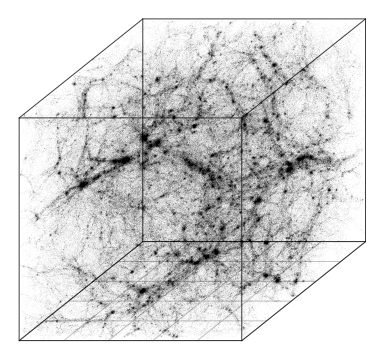
\includegraphics[width=\linewidth]{figure_1_whole_wdm.png}
    \label{fig:introDataCDM}
  \end{subfigure}
    \begin{subfigure}{.40\textwidth}
    \centering
    \caption{Eagle WDM Simulation}  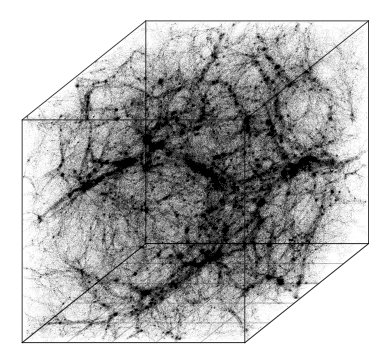
\includegraphics[width=\linewidth]{figure_1_whole_cdm.png}
    \label{fig:introDataWDM}
  \end{subfigure}
    \caption{EAGLE simulation under (a) CDM and (b) WDM \citep{schaye2015eagle}. In theory, warm dark matter are hypothesized to travel at faster speeds than cold dark matter. While the main filaments in (a) and (b) suggest similaries in skeletal structure, the faster speeds of (b) may result in disparaties in density as seen by the more condensed groups in (b).}
    \label{fig:introData}
\end{figure}

The purpose of the proposed hypothesis tests is to denote differences in the topology between structures using persistent homology. In this paper, we begin with an introduction to the algebra behind persistent homology followed by the proposed hypothesis testing framework. Then we carry out a simulation study to investigate the performance of the proposed statistics followed by more background on LSS. And finally, we apply the hypothesis tests to quantify the topological disparities between warm and cold DM assumptions. We end with concluding remarks.


%%%%%%%%%%%%%%%%%%%%%%%%%%%%%%%%%%%%%%%%%%%%%%%%%%%%%%%
%% SECTION: TOOLS FROM TDA
%%%%%%%%%%%%%%%%%%%%%%%%%%%%%%%%%%%%%%%%%%%%%%%%%%%%%%%

\section{Tools from TDA Useful for Studying LSS}
\label{sec:tda}
Homology is the study of certain properties of topological spaces, specifically the number of different ordered holes in the space (e.g. connected components, loops, voids). Persistent homology studies the spacial structure of a parameterized family of topological spaces (e.g., keeping track of the so-called
births and deaths of homological features as a topological space changes with a varying parameter).
%
The type of data we are investigating is a point cloud, where each point can represent a galaxy or, for cosmological simulation data, a certain mass of DM.
With cosmological simulations,  we look at cubic regions representing some part of our Universe and analyze the distribution of matter within that cube. We may define a simplicial complex directly on the point cloud, or we may compute a smoothed version of the data using kernel density estimation (KDE). The homological features mentioned above have cosmological interpretations in dimensions zero, one, and two. We discuss this briefly before going further into the algebraic topology.

\paragraph{Clusters}
A \emph{connected component}, or zeroth-dimensional homology feature ($H_0$), is a maximal subspace of a topological space that cannot be covered by two disjoint open sets. In words, a connected component is a \textit{piece} of a topological space.  If our topological space is a $k$-nn graph, then the components are clusters of data points. In cosmology, these clusters of galaxies (or other cosmological matter) are an important structure to understand. Persistent homology tracks the appearance of new connected components and the merging of two distinct components into one.

\paragraph{Filaments and Loops} A \emph{loop}, or one-dimensional homology feature ($H_1$), provides information about the connectivity of data. As many $H_0$ features appear, nearby connected components can merge together. If our topological space is a $k$-nn graph, then loops are clusters of data points that merge into a fully connected cycle. For LSS, this would appear as filaments joining together in a loop.


\paragraph{Cosmological Voids}  A \emph{void}, or two-dimensional homology feature ($H_2$), represents empty areas within the topological space. If our topological space is a $k$-nn graph, then the voids are the unfilled spaces inside enclosed $H_1$ features.  In cosmology, to fully appreciate the topology, it is important to understand the high-density regions (connected components and loops) but also where matter is scarce.

\subsection{Persistent Homology}
Various methods can be used in order to transform a discrete point set into a topological space. For example, points can be connected based on a distance (or
a distance-like structure as in \citep{chazal2011geometric}), or one may estimate the density from which the points were sampled. In the latter case, one can look at a KDE of a point cloud and study the topological features of super-level sets of that density. Below, we summarize some of the key components of persistent homology. See \citep{edelsbrunner2010computational,hatcher2002algebraic,munkres1984elements} for a more thorough introduction to algebraic and computational topology.

\paragraph{Filtrations}
To derive the persistent homology for $p$, let there exist a threshold $r$, represented by a hyperplane that divides $p$ into two separate segments: a super-level set, defined as $\{(x,y,z) \in p \textup{ s.t. } z \geq r \}$, and a sub-level set $\{(x,y,z) \in p \textup{ s.t. } z < r \}$. If $r$ is initialized at $\infty$, then the super-level set is empty and the sub-level set contains all of $p$. The evolving topological space is characterized by its homology as~$r$ decreases to $-\infty$. The persistent homology would then track the connected components ($H_{0}$), loops ($H_{1}$), and voids ($H_{2}$) that appear and disappear in the super-level sets $p^{-1}([r,\infty)]$. More specifically, as~$r$ intersects $p$, the super-level set is no longer empty and is instead, composed of disjoint maxima. An example of a density with a 2-dimensional domain is presented in Figure~\ref{fig:example_3d}, along with the plane representing a threshold for defining super-level sets.  Figures~\ref{fig:example_contour1} and \ref{fig:example_contour2} display the upper-level sets for two thresholds.  Figure~\ref{fig:example_pd} whos the persistence diagram which is discussed below.


\paragraph{Tracking Homology Generators}
Figure~\ref{fig:example_contour1} and Figure~\ref{fig:example_contour2} show the threshold, $r$ decreasing from 1.1 to 0.1. In that interval, the upper-level set changed from having six connected components ($H_0$'s) and zero loops ($H_1$'s) to having one connected component and one loop. The time in the filtration when homology features appear, the \emph{birth} of the feature, and the time when a feature joins other features, the \emph{death} of the feature, are captured in a persistence diagram. Figure~\ref{fig:example_pd} displays the persistence diagram for the function in Figure~\ref{fig:example_3d}, where each point represents the birth time (x-axis) and death time (y-axis) of a homological feature. A point $(x,x)$ on the diagonal represents a feature with a lifespan of 0.

The \emph{persistence} of a point $(b,d)$ is the length of the interval of the persistence parameter that supports that feature: $d-b$. In the persistence diagram, the distance from $(b,d)$ to the diagonal is proportional to this value; in fact, the (Euclidean) distance to the diagonal is $\frac{(b-d)}{\sqrt{2}}$. Often, the persistence of a feature is indicative of the significance of the feature, which means that points close to the diagonal are indistinguishable from noise.

\begin{figure}
  \begin{subfigure}{.27\linewidth}
    \centering
    \caption{}
        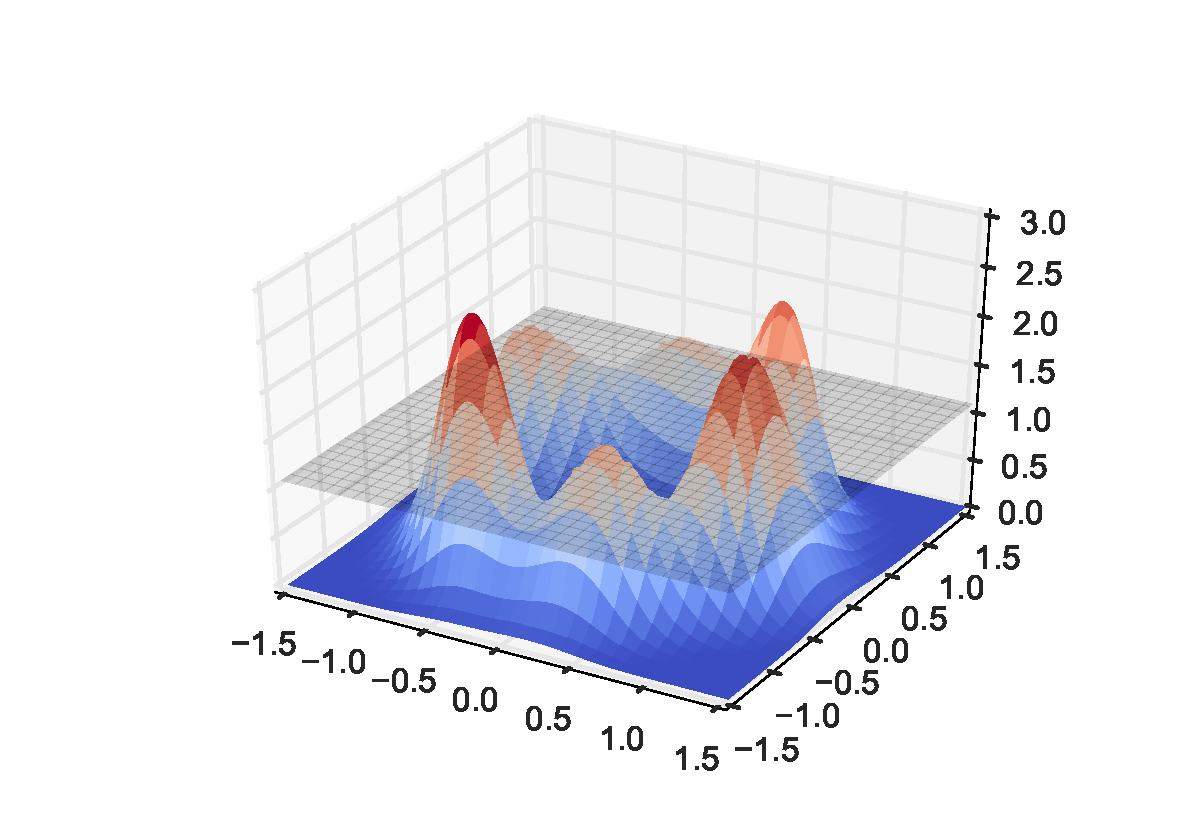
\includegraphics[width=\linewidth]{figure_2_3d_repr.pdf}
    \label{fig:example_3d}
  \end{subfigure}
    \begin{subfigure}{.25\linewidth}
    \centering
    \caption{}
        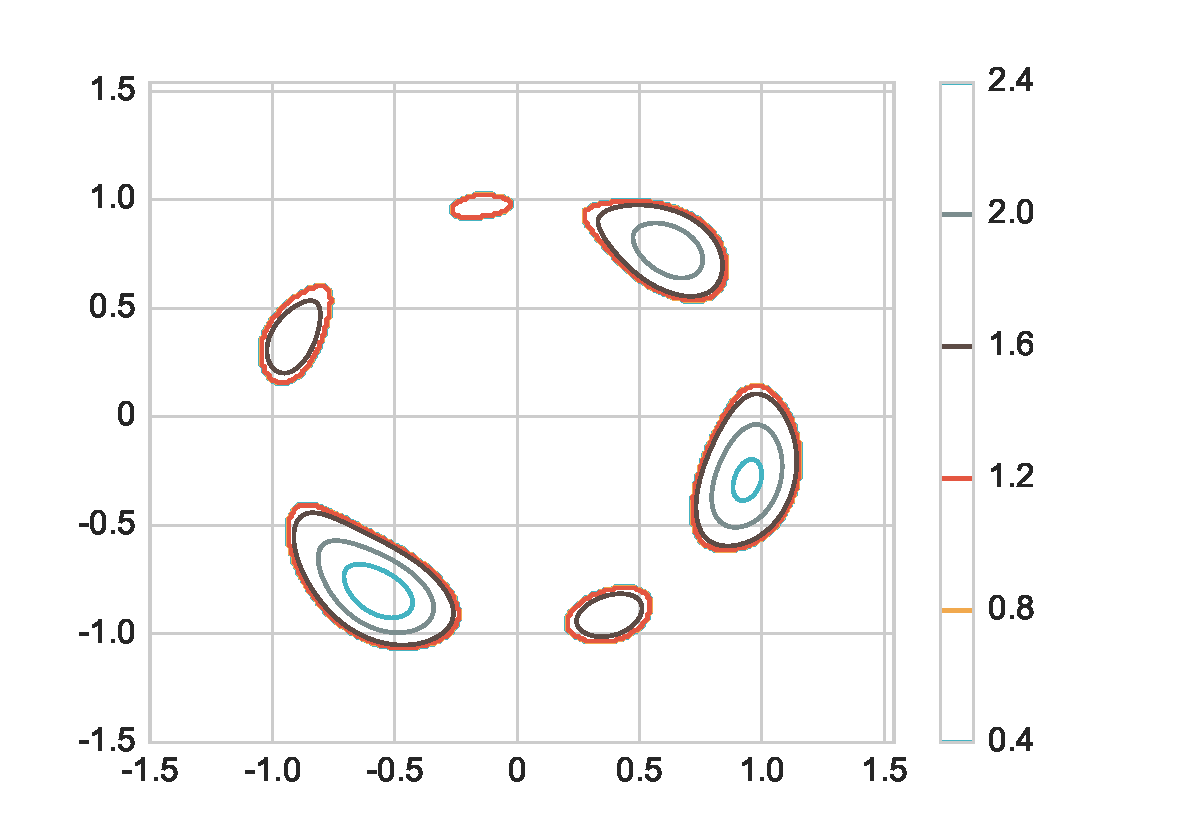
\includegraphics[width=\linewidth]{figure_2_contour_1.pdf}
    \label{fig:example_contour1}
  \end{subfigure}
    \begin{subfigure}{.25\linewidth}
    \centering
    \caption{}
        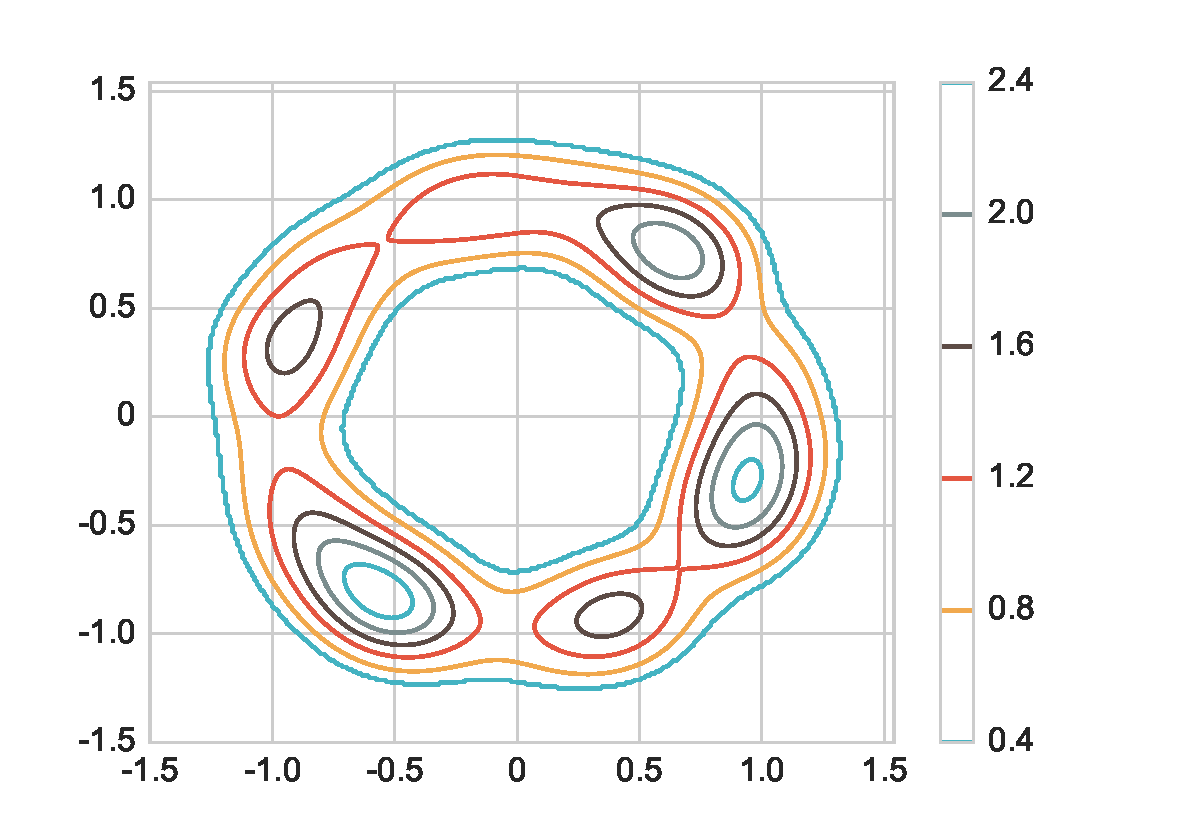
\includegraphics[width=\linewidth]{figure_2_contour_2.pdf}
    \label{fig:example_contour2}
  \end{subfigure}
    \begin{subfigure}{.20\linewidth}
    \centering
    \caption{}
        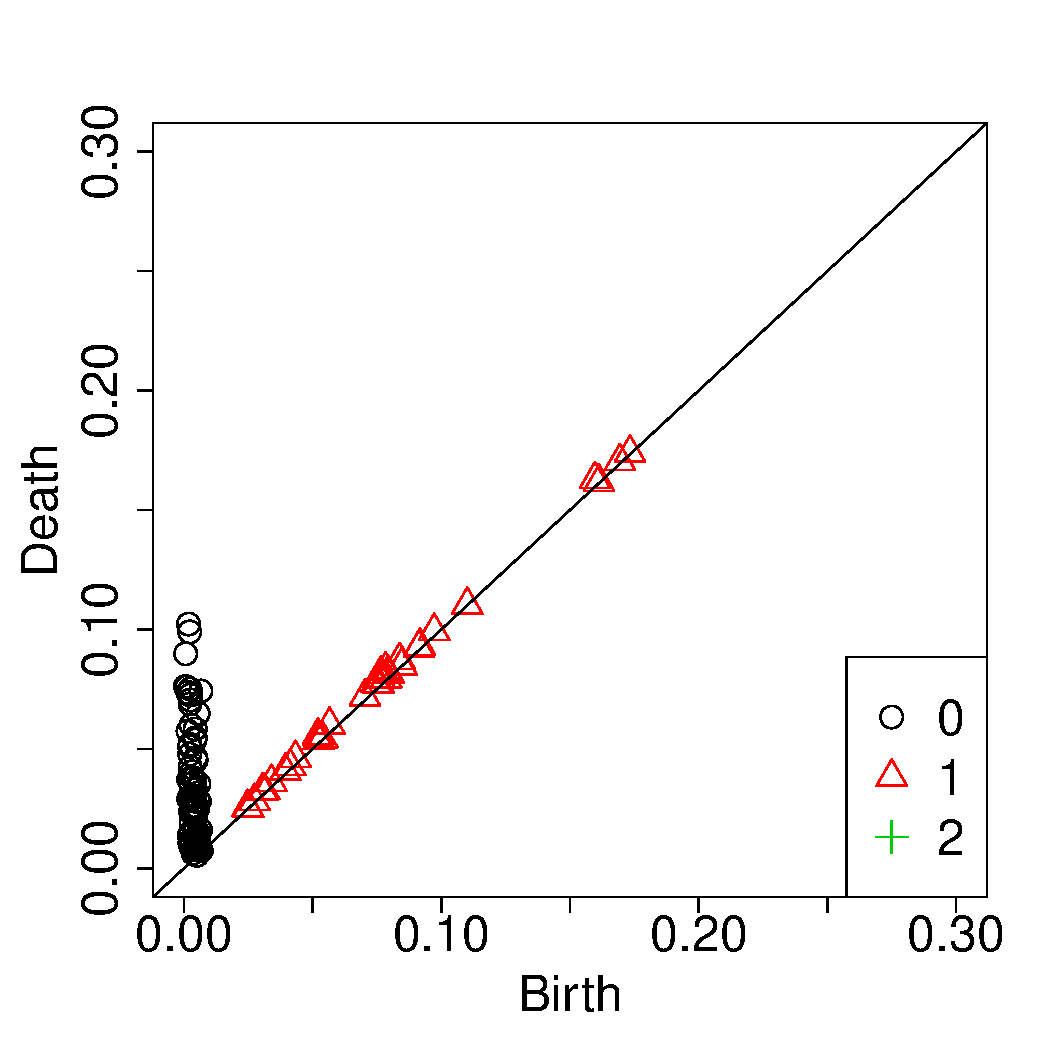
\includegraphics[width=\linewidth]{figure_2_pd.pdf}
    \label{fig:example_pd}
  \end{subfigure}
  \caption{ We illustrate persistent homology with a two-dimensional example. The density in (a) shows 3 steep peaks and 3 shallow peaks  distributed around a uniform circle. In light gray, we see the hyperplane, shown (b) as $t=1.0$. (b) and (c) plot the super-level sets $\widehat{p}^{-1}[1.10,\infty)$ and $\widehat{p}^{-1}[0.10,\infty)$ respectively. Notice that as the threshold is decreased, the contour more clearly defines a loop-like structure. In (d), we see the persistence diagram for the super-level set filtration of $\widehat{p}$. We highlight the upper left quadrant based at $(0.18, 0.02)$, which contains a one-dimensional persistence point. This corresponds to the loop shown in (c). The remaining 0-dimensional homologies represent the connected components from each of the 6 peaks.} % end caption
    \label{fig:homologyexample}
\end{figure}

%\paragraph{An Example}
%In order to illustrate persistent homology, we step down a dimension from cubes in $\R^3$ to squares in $\R^2$. In \figref{fig:homologyexample}, we see how persistent homology captures the evolving super-level sets of a KDE $\widehat{p} \colon [-2,2]^2 \to \R$.  The density plot in \figref{fig:homologyexample} was created using 6 Gaussian peaks distributed along a uniform circle in the $<x,y>$ plane. As the persistence parameter $t$, shown as a hyperplane in \figref{fig:homologyexample}(a), decreases from $\infty$ to $-\infty$, various events occur in the super-level sets $\widehat{p}^{-1}[t,\infty)$: a new component can appear (zeroth-dimensional birth), two distinct components can merge (zero-dimensional death), a loop can appear (one-dimensional birth), and two loops can become homologous (one-dimensional death).  These birth and death events are paired and plotted in the persistence diagram.
%%
%In the persistence diagram of \figref{fig:homologyexample}(a), we see exactly 6 zero-dimensional persistence points (denoted by black circles), one for each of the Gaussian peaks, and a single one-dimensional persistence point (denoted by red triangles), representing the circle on which the modes are located and is captured in \figref{fig:homologyexample}(c).
%
%The upper-left quadrant based at a point $(x,x)$ will contain all persistence points that are born before $x$ and die at or after $x$; that is, the persistence points in this quadrant are in one-to-one correspondence with generators of $p^{-1}(x,\infty)$.  In this way, the homology of each super-level set can be read off of the persistence diagram.
%\brittany{todo: continue here (update for new example)}

\subsection{Derivatives of Persistence Diagrams}
While persistence diagrams can summarize the topology of a data set, it is not straightforward to compare two different persistence diagrams. Often simpler metrics like the bottleneck distance or the $q$-Wasserstein distance are used in this setting, but are computationally expensive. Below are several examples of methods to further summarize a persistence diagram that will be used in \ref{sec:methods} to develop hypothesis tests.

\paragraph{Landscapes and Silhouettes}
Weighted silhouette functions are formed by weighting a particular functional summary of persistence diagrams called \emph{landscape functions} \citep{bubenik2015statistical}. More details and theoretical properties of landscapes and silhouettes are provided in \citep{chazal2014stochastic}.

Landscape functions are defined as follows. Let the finite birth and death intervals of a persistence diagram with $n_h$ points, for homology dimension $h = 0, 1, 2, \ldots$, be defined as $\{(b_{hi},d_{hi})\}_{i = 1}^{n_h}$.  Next, consider rotating the persistence diagram such that a given point is $p_{hi} = \left(\frac{b_{hi}+d_{hi}}{2}, \frac{d_{hi}-b_{hi}}{2}\right) \in D_h, \quad i = 1, \ldots, n_h$.  Equilateral triangles are formed from each $p_{hi}$ to the base as
\begin{equation*}
\Lambda_{p_{hi}}(t) =
  \begin{cases}
    t - b_{hi}  & \quad t \in [b_{hi}, \frac{d_{hi}+b_{hi}}{2}]\\
    d_{hi} - t  & \quad t \in [\frac{d_{hi}+b_{hi}}{2}, d_{hi}]\\
    0  & \quad \text{ otherwise}\\
  \end{cases}
\end{equation*}
where $t \in [t_{\min}, t_{\max}]$. For a given $h$, the persistence landscape is then defined as the following collection of functions

\begin{equation*}
\lambda_{D_h}(k, t) = \underset{p_{hi}\in D_h}{\text{kmax }} \Lambda_{p_{hi}}(t), \quad t \in [t_{\min}, t_{\max}], k = 1, \ldots, n_h
\end{equation*}
where kmax is the kth largest value in $D_h$.  An example of a landscape function is displayed in Figure~\ref{fig:landscape}.

\begin{center}
\begin{figure}[htp!]
  \centering
  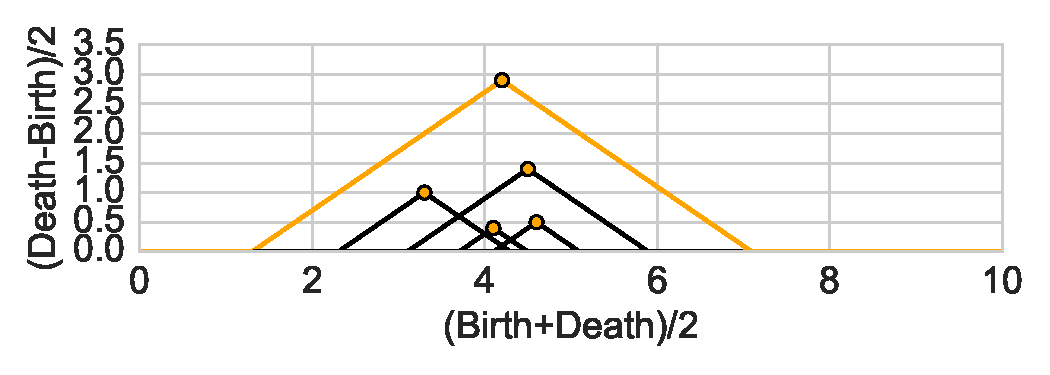
\includegraphics[width=0.6\linewidth]{figure_3_silh.pdf}
    \caption{An example of a landscape function. The points shaded in color represent the homology coordinates in a persistence diagram $D$. The landscape $\lambda(k, \cdot)$ is the $k$-th largest of the arrangement of the graphs of $\left \{ \Lambda_{p} \right \}$. In particular, the orange and blue segment represent landscape $\lambda(1, \cdot)$ and $\lambda(2, \cdot)$ respectively, with $\lambda(1, \cdot)$ denoted as the largest landscape function. A weighted silhouette function weighs the landscapes $\lambda(k, \cdot)$ into a single continuous function.}
    \label{fig:landscape}
\end{figure}
\end{center}

Rather than working with each $k$ of $\lambda_{D_h}(k, t)$ individually, silhouettes provide a way of combining the information in the collection of landscape functions. Silhouettes are weighted averages of the individual functions for homology dimension $h$ defined~as
%
\begin{equation*}
\phi_h(t) = \frac{\sum_{i = 1}^mw_{hi}\Lambda_{hi}(t)}{\sum_{i = 1}^mw_{hi}}
\end{equation*}
where the weights $w_i$ can give more emphasis or less emphasis to features with longer lifetimes. As suggested in \citep{chazal2014stochastic}, we use $w_{hi} = |d_{hi} - b_{hi}|^p$, where $p$ is a tuning parameter that needs to be selected.

\paragraph{Euler Characteristic Function}
The Euler characteristic is a topological invariant and defined as: $\chi = \beta_{0} - \beta_{1} + \beta_{2} - \beta_{3} + ... \pm \beta_N = \sum_{i=0}^{N} (-1)^{i} \beta_{i}$,
where $\beta_{i}$ represents the $i$-th Betti number (the rank of the $i$-th homology group) and $N$ is the number of dimensions. When analyzing persistence diagrams of LSS, since there exist only three dimensions of data, the only non-trivial homology groups will be in dimensions 0, 1, and 2. Given the Betti numbers $\beta_{0}$, $\beta_{1}$, and $\beta_{2}$, the Euler equation simplifies to:
$\chi = \beta_{0} - \beta_{1} + \beta_{2}.$
The topological space is parameterized by the threshold, $t$ (ranging from $t_{\min}$ to $t_{\max}$), defining the upper-level sets. The Euler Characteristic function, $\chi(t)$, captures the Euler characteristic for each threshold $t$.

%%%%%%%%%%%%%%%%%%%%%%%%%%%%%%%%%%%%%%%%%%%%%%%%%%%%%%%
%% SECTION: METHODS
%%%%%%%%%%%%%%%%%%%%%%%%%%%%%%%%%%%%%%%%%%%%%%%%%%%%%%%

\section{Methods}
\label{sec:methods}
In this section, we describe several frameworks for using persistence diagrams in two-sample hypothesis tests to compare differences between sets of data in topological structure.

\begin{sloppypar}
Suppose we have two sets of persistence diagrams, $\{\mathcal P_1^{(1)}, \ldots, \mathcal P_{n_1}^{(1)}\}$ and $\{\mathcal P_1^{(2)}, \ldots, \mathcal P_{n_2}^{(2)}\}$.  These samples can be used to test $H_0: \mathcal
P^{(1)} = \mathcal P^{(2)}$ vs. $H_1: \mathcal P^{(1)} \neq \mathcal P^{(2)}$, where $\mathcal P^{(1)}$ and $\mathcal P^{(2)}$ are the true underlying
distributions of persistence diagrams for group 1 and 2, respectively.  Properties of probabilities on a space of persistence diagrams are addressed in \citep{Mileyko:2011aa}. We would like the framework to test the hypothesis that the two samples are drawn from populations with different random topologies. However, we note that without incorporating a scaling adjustment on the space of the data or the space of the diagrams, geometrical differences can also lead to a rejection of the null hypothesis. This is discussed in more detail in Section~\ref{sec:standardize}.
\end{sloppypar}

Given two samples of persistence diagrams, there are a number of possible ways to derive test statistics. We consider four general approaches. The first approach is based on functional summaries derived from the sampled persistence diagrams: Euler characteristic function (EC), Silhouette function (SIL), and a
Silhouette-Euler characteristic function (SILEC). Given that each observed dataset will have a corresponding function, a \emph{p-value} can be derived from a two-sample T-test based by integrating the absolute value of the functional summaries. The next two approaches use variations on smoothed persistence diagrams called \emph{intensity functions} \citep{chen2015statistical} with p-values derived from a two-sample kernel test \citep{gretton2012kernel} and an asymptotic argument through permutation (IK, WIK, PI). Additionally, we consider a test using the two-point correlation function (CORR) in order to have a comparison with a summary directly capturing the spatial behavior of the LSS. Similar to the functional summaries above, p-values for the CORR test will be carried out with a T-test based on the integral of the absolute value of the correlation function. The proposed test statistics are discussed in more detail below.

% Given any persistence diagram $x$ extracted from a point cloud, $x$ represents a sample from some latent distribution $\chi$. For example, given a simulation of the Megaparsec cosmic mass, the $(x, y, z)$ points are discrete samples from the continuous, observable Universe, which represents the true distribution. Using that definition, suppose there are two persistence diagrams, $x$ and $y$, each produced from a separate point cloud. Given that $x \sim \chi$, and $y \sim \gamma$, where $\chi$ and $\gamma$ represent the true distributions, an interesting question is whether $\chi$ and $\gamma$ are identical to some error $\epsilon$. In other words, are the samples $x$ and $y$ sampled from the same latent distribution? One might consider the following hypothesis test, where $H_{0}$ is the null and $H_{A}$ is the alternative.

% \[ H_{0} : \chi = \gamma \]
% \[ H_{A} : \chi \neq \gamma \]

% However, given that the parameters of the distributions $chi$ and $\gamma$ are unknown, one cannot directly compare them. Instead, one much infer the relationship between $chi$ and $gamma$ by comparing the diagrams sampled from $\chi$ and $\gamma$ respectively. Given $n$ samples, a hypothesis test should be designed to compare $\{ x_{1}, ..., x_{n} \sim \chi \}$ and $\{ y_{1}, ..., y_{n} \sim \gamma \}$. However, comparing two persistence diagrams, $x$ and $y$, is non-trivial. Naive distance calculations, like bottleneck or Wasserstein, are easily perturbed by randomness and noise, and are computationally expensive. Instead, we propose to further summarize a persistence diagram by a test statistic. To find such a test statistic, we must define a function $f_{T}$ that takes an input $x$ and produces a statistic $T_{x}$, $f_{T}(x) = T_{x}$. Provided such a function exists, using the further summarized statistics, we can test the hypothesis that two persistence diagrams, $x$ and $y$ are sampled from the same latent distribution with the following framework:

% \[ H_{0} : f_{T}(x) = f_{T}(y) \]
% \[ H_{A} : f_{T}(x) \neq f_{T}(y) \]

% One main contribution of this paper is studying the effectiveness of different functions $f_{T}$ when the true topological relationship between $x$ and $y$ are known. The best functions $f_{T}$ are then used to analyze a data set in which the topological relationships is unknown. We now proceed to describe different methods for defining $f_{T}$ for hypothesis testing in the setting of large-scale structure (LSS).

Among the variations to test statistics considered (EC, SIL, SILEC, IK, WIK, PI, and CORR), we are seeking the summary that is most sensitive to differences in distributions of persistence diagrams produced from LSS.

\paragraph{Euler Characteristic Test (EC)}
Each persistence diagram in the two samples result in an individual Euler characteristic (EC) function, $\chi^{(J)}(t)$,  $J = 1, 2$. The two-sample T-test is based on the following sample means:
\begin{equation*}
\frac{1}{n_J}\sum_{i = 1}^{n_J} \int_{t_{\min}}^{t_{\max}} | \chi_i^{(J)}(t) | \textup{ d}t.
\end{equation*}

\begin{figure}[htbp]
   \centering
  \begin{subfigure}{.24\textwidth}
    \centering
        \caption{Point Cloud}
        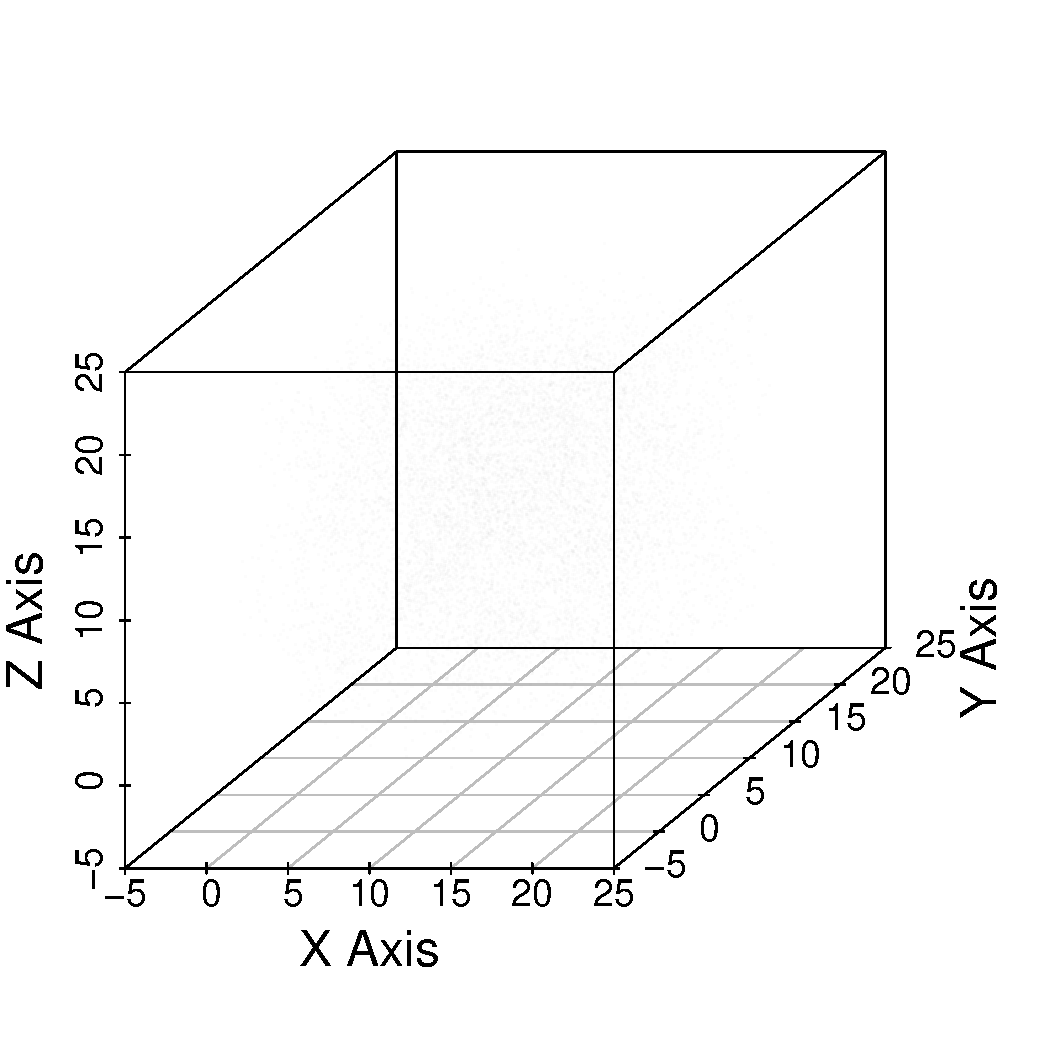
\includegraphics[width=\linewidth]{figure_5_plot.pdf}
    \label{fig:examplestest1}
  \end{subfigure}
    \begin{subfigure}{.24\textwidth}
    \centering
        \caption{PD}
        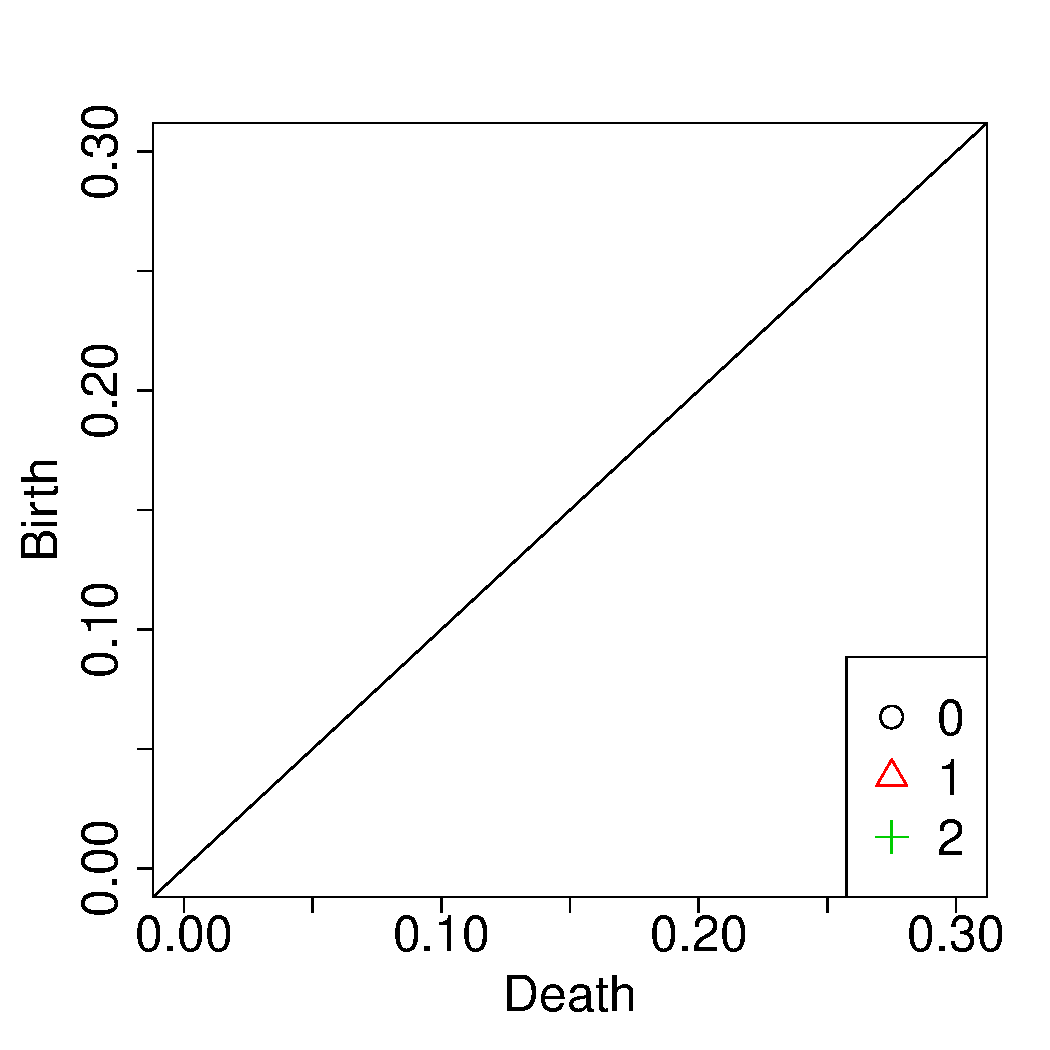
\includegraphics[width=\linewidth]{figure_5_pd.pdf}
    \label{fig:examplestest2}
  \end{subfigure}
    \begin{subfigure}{.24\textwidth}
    \centering
        \caption{EC}
        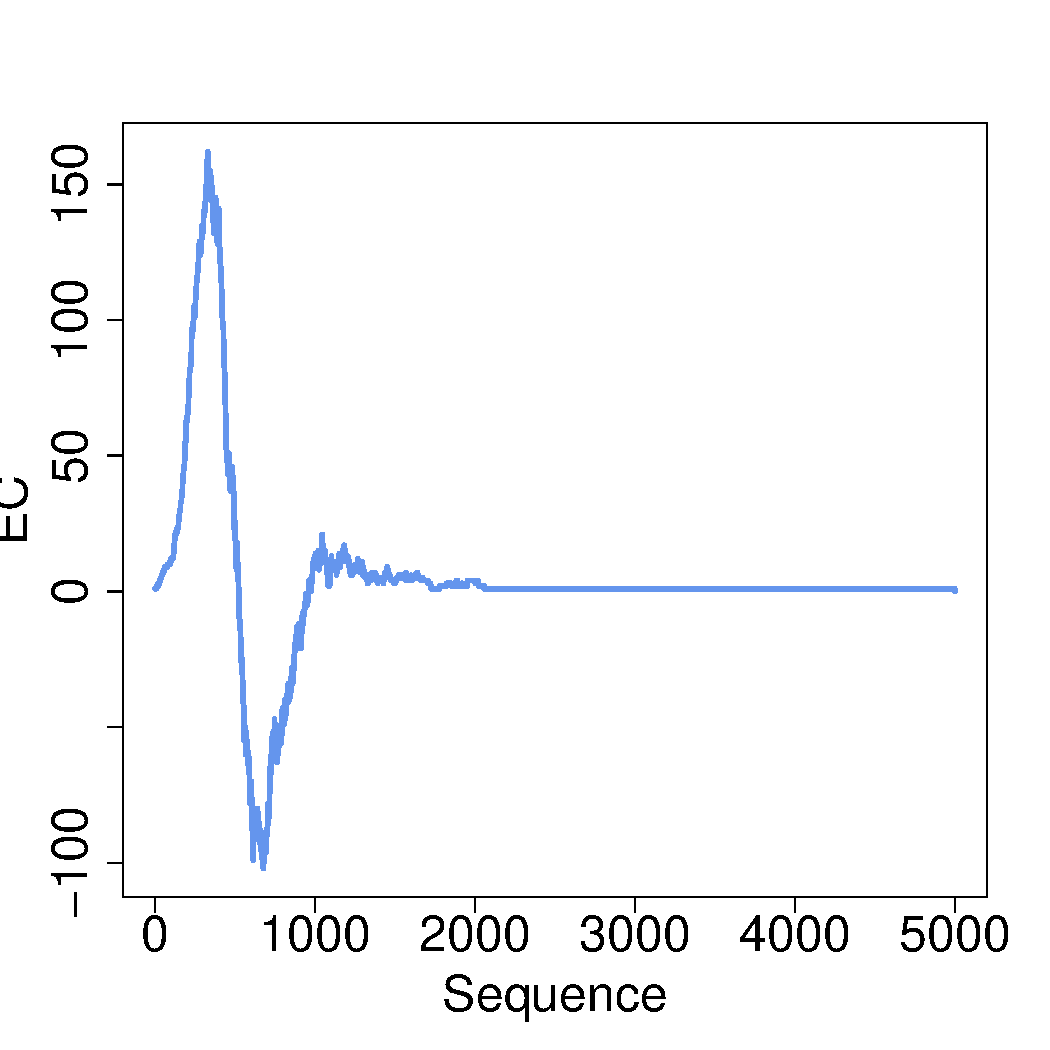
\includegraphics[width=\linewidth]{figure_5_euler.pdf}
    \label{fig:examplestest3}
  \end{subfigure}
    \begin{subfigure}{.24\textwidth}
    \centering
        \caption{SIL}
        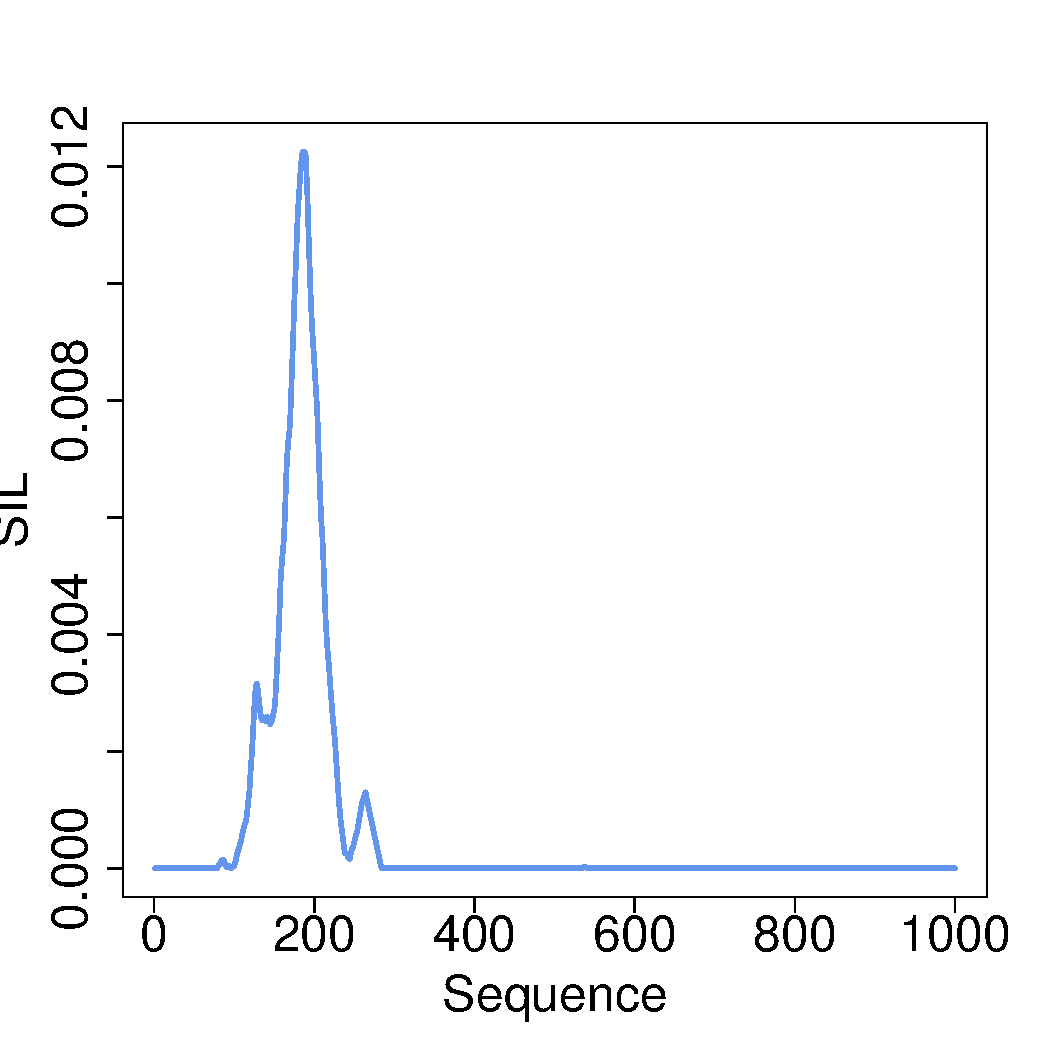
\includegraphics[width=\linewidth]{figure_5_silhouette.pdf}
    \label{fig:examplestest4}
  \end{subfigure}
    \begin{subfigure}{.24\textwidth}
    \centering
        \caption{IK}
        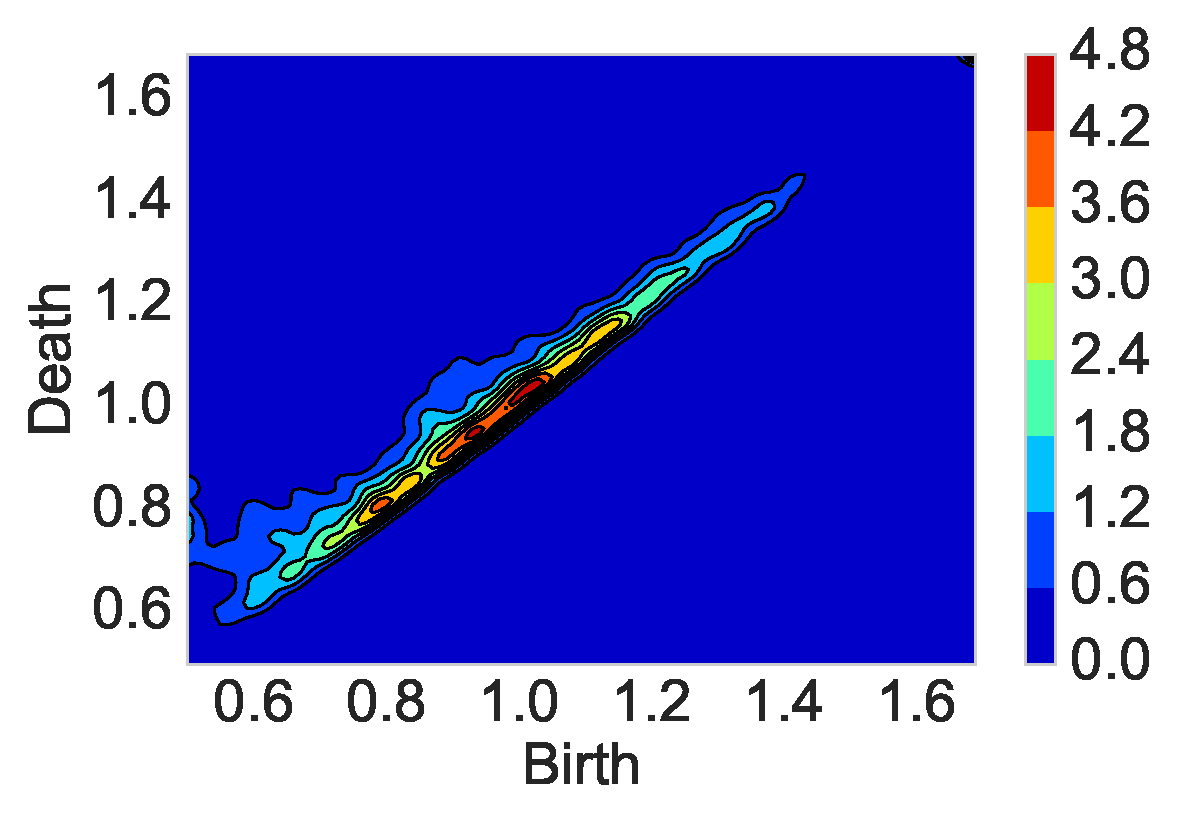
\includegraphics[width=\linewidth]{figure_5_kernel.pdf}
    \label{fig:examplestest5}
  \end{subfigure}
    \begin{subfigure}{.24\textwidth}
    \centering
        \caption{CORR}  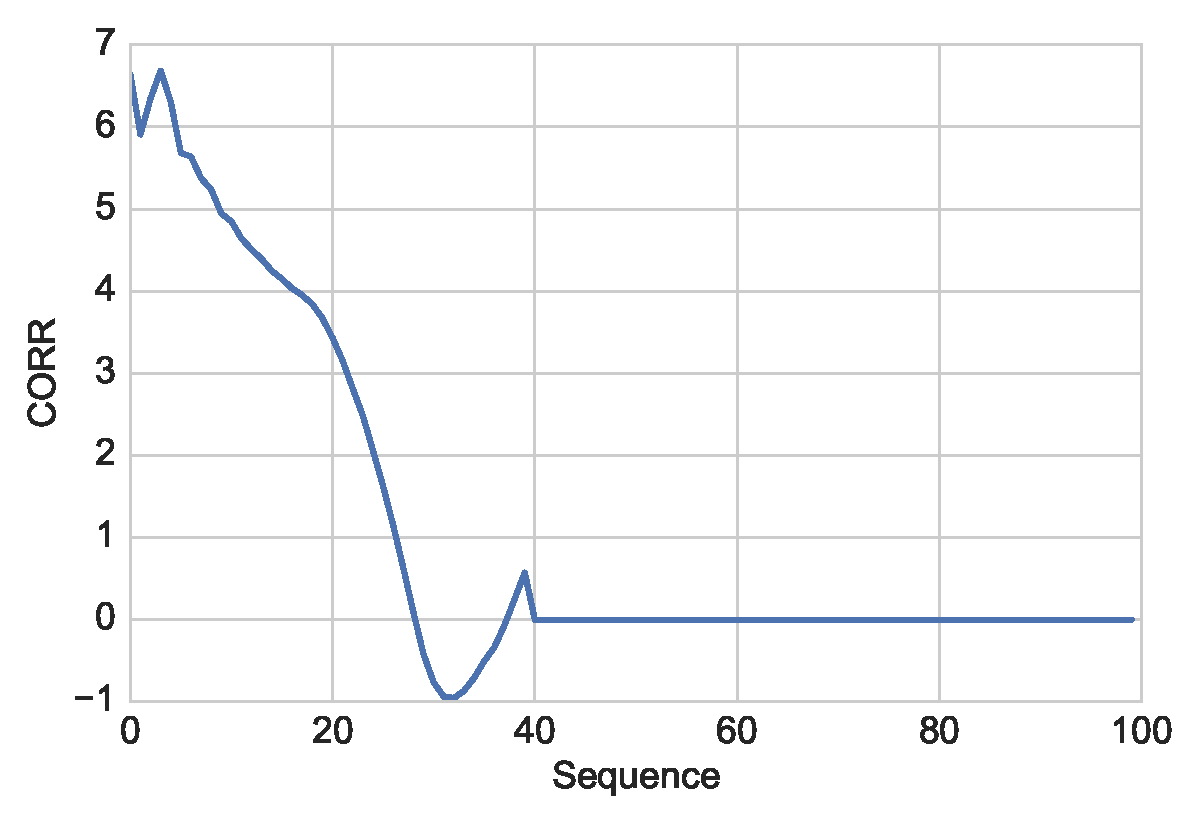
\includegraphics[width=\linewidth]{figure_5_corr_fun.pdf}
    \label{fig:examplestest6}
  \end{subfigure}
    \begin{subfigure}{.24\textwidth}
    \centering
        \caption{WIK}
        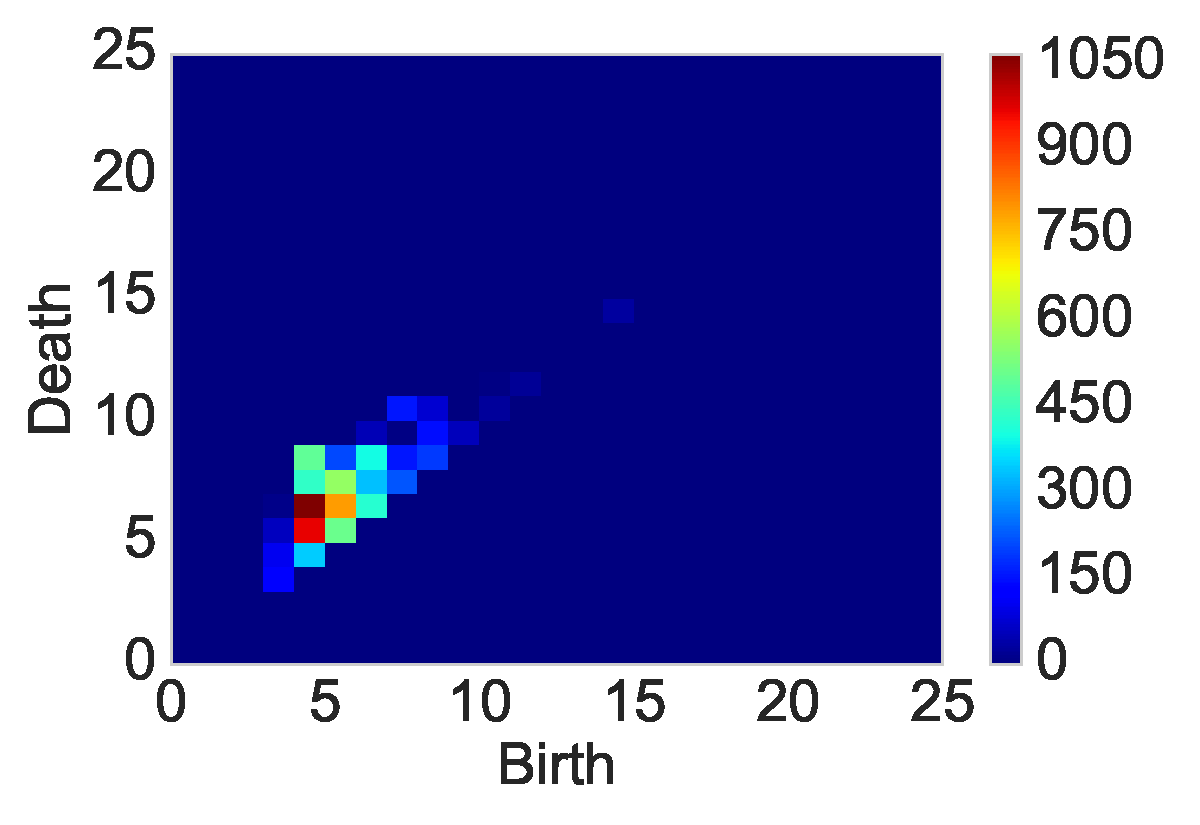
\includegraphics[width=\linewidth]{figure_5_intensity_fun.pdf}
    \label{fig:examplestest7}
  \end{subfigure}
    \begin{subfigure}{.24\textwidth}
    \centering
        \caption{PI}
        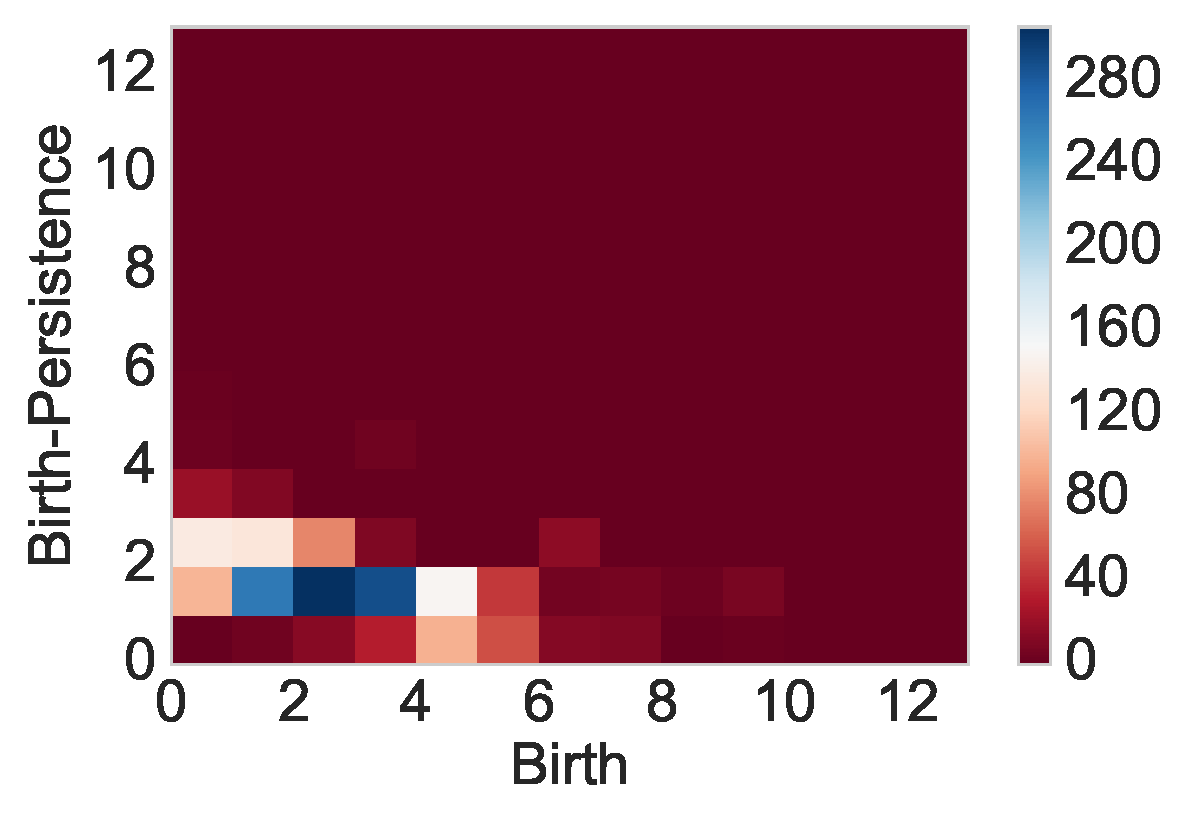
\includegraphics[width=\linewidth]{figure_5_pimage_fun.pdf}
    \label{fig:examplestest8}
  \end{subfigure}
   \caption{Examples of eight test statistics used in the hypothesis tests. A Voronoi foam with a percent filament of 0.5 generates the point cloud dataset shown in (a). Visually, (a) shows dense and sparse regions of sampled points that produce the topological signatures shown in (b). (b) contains three homology features, where 0, 1, and 2 represent connected components, loops, and voids respectively. (c) shows the euler characteristic function derived from the (b) as an alternating sum of Betti numbers. (d) shows the weighted silhouette of the landscape functions. See \figref{fig:landscape} for more details. (e), the intensity kernel, smooths a persistence diagram using a 1-D Gaussian kernel. Because points further from the diagonal are more topologically interesting, (g) builds on (e) by weighting points closer to the diagram less in order to prevent over-smoothing. (h) is similar to (g) but performs a linear transformation on both axis and uses a 2-D Gaussian on all 3 homologies together. (f) shows the two-point correlation function, which summarizes (a) directly without (b). See Section \ref{sec:methods} for more details.}
   \label{fig:examples}
\end{figure}

% \begin{center}
% \begin{figure}[htp!]
%   \centering
%   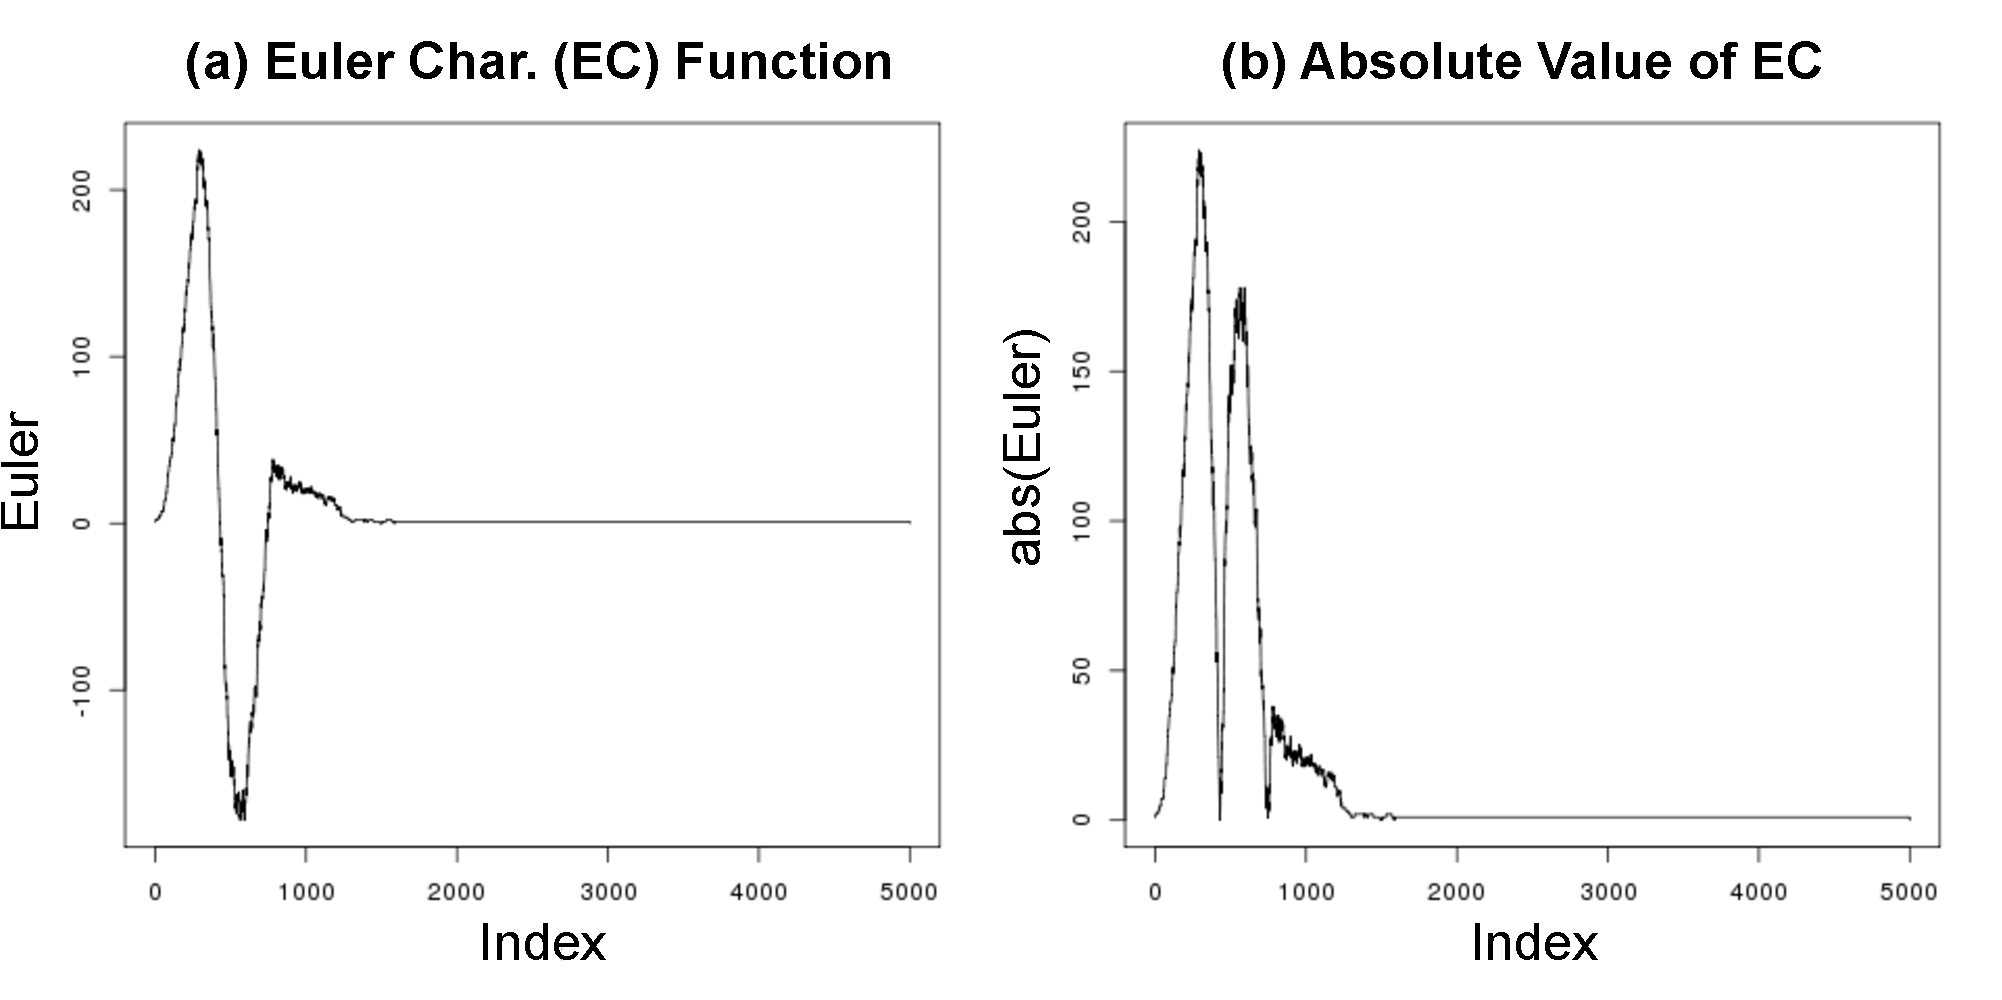
\includegraphics[width=0.7\linewidth]{example_euler.pdf}
%     \caption{(a) An Euler characteristic function created by plotting the Euler characteristic of a Voronoi foam model at each point beginning at time 0 until the last birth time. (b) The absolute value of the characteristic function that is integrated to produce the test statistic $E_{t}$.}
%     \label{fig:eulerexample}
% \end{figure}
% \end{center}

\paragraph{Silhouette Test (SIL)}
As with the Euler Characteristic (EC) function, a weighted silhouette summarizes a persistence diagram through a continuous function. And as with EC, a two-sample T-test is carried-out by integrating the weighted silhouette functions for each sample.  However, the $SIL$ tests are carried out individually for each homology dimension, $h = 0, 1, 2$, resulting in $SIL_0$, $SIL_1$, and $SIL_2$. In an effort to combine information across homologies, we also considering Hotelling's $T^2$ test using the all three dimensions at once, denoted $SIL_{0:2}$.


\paragraph{Silhouette-Euler Characteristic (SILEC).}
Another method for simultaneously considering individual silhouettes, $S_{h}(t)$, across dimensions $h = 0$, 1, and 2, is a modified Euler characteristic function. Instead of calculating the alternating sum of Betti numbers, the Silhouette-Euler characteristic function (SILEC) computes the alternating sum of  individual silhouette functions across the threshold parameter, $t$, $SILEC(t) =  S_{1}(t) - S_{2}(t) + S_{3}(t)$. A p-value is calculated using a T-test in the same fashion as done for EC.




%\paragraph{Permutation Method.} Although not one of the nine approaches, the permutation method is frequently used in our tests and provides a very generic approach for calculating a p-value from any arbitrary test statistic. Assuming we observe two independent samples $X_{1}, \cdots, X_{n} \sim P$ and $Y_{1}, \cdots, Y_{n} \sim Q$, the two sample test problem is to test the hypothesis $H_{0} : P = Q$ versus the alternative $H_{1} : P \neq Q$. Assuming there is some arbitrary method of calculating a test statistic $T$ as a function of the data, we reject $H_{0}$ if $T > t$ where $t$ is a critical value. We choose $t$ such that if $H_{0}$ is true then $W(T > t) \leq \alpha$ where $W$ is the distribution of $T$ when $H_{0}$ is true. Permutation testing attempts to help us choose $t$ and find $W$ of $T$ under $H_{0}$.
%
%In the permutation method, the data is concatenated as a vector in the order \[X_{1}, X_{2}, \cdots, X_{n}, Y_{1}, Y_{2}, \cdots, Y_{n}\] and presented initial labels of $0$ or $1$ where all $X_{i}$ receive label 0 and all $Y_{i}$ receive label 1. If $H_{0}$ is true, then the entire data vector is an i.i.d sample from $P$ and the group labels are arbitrary. To test this, the group labels are randomly permuted and the test statistic is recalculated. This changes the values of $T$ but (under $H_{0}$), it should not change the distribution of $T$. The labels are permuted $N$ times and the p-value is
%
%\[ p = \frac{1}{N}\sum^{n}_{j=1} I(T_{j} \geq T) \]
%
%where $I$ is the indicator function. Therefore, the p-value is the fraction of times $T_{j}$ is larger than $T$. As $N$ approaches $\inf$, $p$ approaches the exact value.

\paragraph{Intensity Kernel Test (IK).}
Rather than working with raw persistence diagrams, the Intensity Kernel Test (IK) smooths the diagrams with a Gaussian kernel, similar to the intensity function seen in \citep{chen2015statistical}. The test statistic is derived using a kernel two-sample test. The IK statistic used in this paper is computed for two sets of persistence diagrams, and the discrepancy between the diagrams is calculated as the integrated squared difference between two \emph{unweighted} intensity functions instead of points directly from the persistence diagrams. (Unweighted intensity functions assigns uniform weights to points on the diagram and therefore does not account for the diagonal boundary on persistence diagrams where birth = death; we considered weighted intensity functions next.) The two-sample test statistic for $X = X_1, \ldots, X_{n_1}$ and $Y = Y_1, \ldots, Y_{n_2}$ is defined as
%
\begin{equation}
\widehat{T}_{IK}(X, Y) = \frac{1}{n_1^{2}}\sum_{i=1}^{n_1}\sum_{j=1}^{n_1} K_{\sigma}(X_{i}, X_{j}) - \frac{2}{n_1n_2}\sum_{i=1}^{n_1}\sum_{j=1}^{n_2}K_{\sigma}(X_{i}, Y_{j}) + \frac{1}{n_2^{2}}\sum_{i=1}^{n_2}\sum_{j=1}^{n_2} K_{\sigma}(Y_{i}, Y_{j}), \label{eq:kernel_test}
\end{equation} where $n_1$ and $n_2$ are the sizes of the two samples, and $\{X_1, \ldots, X_{n_1}\}$ and $\{Y_1, \ldots, Y_{n_2}\}$ are the two sets of intensity functions.  $K_{\sigma}(X,Y)$ can be thought of as a similarity measure between intensity functions $X$ and $Y$, and in this case is a Gaussian kernel $K_{\sigma}(X,Y) = exp(-\frac{||X - Y||^{2}}{\sigma^{2}})$ with  $||X - Y|| = \int \left(X(t_1, t_2) - Y(t_1, t_2)\right)^2dt_1dt_2$. The $\sigma$ is a hyperparameter that sets the standard deviation of the Gaussian distribution used in the kernel $K_{\sigma}$: a larger $\sigma$ will reduce sensitivity to small differences between $X$ and $Y$, while a smaller $\sigma$ will heighten sensitivity. The optimal $\sigma$ value was found to be $0.1 \pm 0.04$ using grid search from 0 to 5. A permutation test is used to calculate a p-value for each homology dimension, $IK_0$, $IK_1$, and $IK_2$.
% with $N$ permutations, and the p-value represents the fraction of times $T_{j}$ is larger than the observed $\widehat{GC}$ for any $j$,

% \[ \text{p-value} = \frac{1}{N} \sum_{j=1}^{N} I(T_{j} \geq T). \]

\paragraph{Weighted Intensity Kernel Test (WIK)}
The intensity function in WIK, unlike IK, uses weighted kernel density estimates \citep{chen2015statistical} where the weights are a function of a point's persistence. Let $(b_i, d_i)$, $i = 1, \ldots, m$ be the features on a persistence diagram corresponding to some dimension $h$. Then the weighted intensity function for the persistence diagram is
%
\[ X(t_1, t_2) = \sum_{j=1}^m(d_{j} - b_{j})\frac{1}{\tau^{2}}K \left(\frac{t_1-d_{j}}{\tau}\right)K \left(\frac{t_2-b_{j}}{\tau}\right)\]
%
such that the sum over all persistent features, $K$ is a symmetric kernel function, and $\tau$ is a smoothing parameter. Using weighted intensity functions, a p-value is calculated by considering the same kernel test statistic as Equation~\eqref{eq:kernel_test} and a permutation test for each homology dimension produces three analogous statistics: $WIK_0$, $WIK_1$, and $WIK_2$.

\paragraph{Persistent Image Test (PI)} The Persistent Image test \citep{adams2015persistent} is a variation of the WIK test with an alternative kernel function and sub-sampling. Again, let $\mathcal{D} = {(b_{j} , d_{j}) : i = 1, \cdots ,m}$ be a persistence diagram where $m$ is the number of persistent features. Unlike WIK, the PI test first transposes the persistent diagram using the linear transformation $T: \mathbb{R}^{2} \rightarrow \mathbb{R}^{2}$ where $T(x,y) = (x, y-x)$. Therefore, let $T(\mathcal{D})$ represent the transformed diagram with the new birth-persistence coordinates. Let $P_{u} : \mathbb{R}^{2} \rightarrow \mathbb{R}$ be a differentiable probability distribution with mean $u = (u_{x}, u_{y})$. In our applications, we choose this distribution to be the normalized symmetric two-dimensional Gaussian with mean $(u_{x}, u_{y})$ and variance $\sigma^{2}$.

\[ P_{u}(x,y) = \frac{1}{2\pi\sigma^{2}}e^{-[(x - u_{x})^{2} + (y-u_{y})^{2}]/2\sigma^{2}} \]

Finally, let $f : \mathbb{R}^{2} \rightarrow \mathbb{R}$ be a non-negative weighting function that is zero along the horizontal axis, continuous and differentiable. $f$ is chosen to only depend on the rotated vertical persistence coordinate $y$, and like WIK, weight points of higher persistence more heavily. In our applications, we use a piecewise linear weighting function that was found to be stable. Given $b > 0$, define $f_{b}$ as

\[ f_{b}(t) = \rightarrow \left\{\begin{matrix}
0 & \textup{if } t \leq 0 \\
\frac{t}{b} & \textup{if } 0 < t < b\textup{, and}\\
1 & \textup{if } t \geq b
\end{matrix}\right. \]

Given $f$, $P$, and $T(\mathcal{D})$, we can define a persistence surface \citep{adams2015persistent}, $\rho_{\mathcal{D}} : \mathbb{R}^{2} \rightarrow \mathbb{R}$ as

\[ \rho_{\mathcal{D}}(x, y) = \sum_{u \in T(\mathcal{D})} f(u)P_{u}(x,y) \]

Like the WIK test, $\rho$ is calculated over the two-dimensional grid \[ \{ (x, y) \textup{ s.t. } b_{min} \leq x \leq b_{max} \wedge d_{min} \leq y \leq d_{max} \} \]. In our applications, the step sizes $h_{x}$ and $h_{y}$ were chosen to make the grid size 30 by 30. Given $\rho_{\mathcal{D}}$, a persistence image \citep{adams2015persistent} $I(\rho_{\mathcal{D}})_{p}$ is defined as a grid of pixels calculated from convolving the persistent surface with a uniform matrix of size $n$ by $n$ of 1's. In order words, $I(\rho_{\mathcal{D}})_{p} = \int\int_{p} \rho_{\mathcal{D}} \textup{ d}y\textup{d}x$. This matrix is then flattened into a 1D vector.  The accuracy of the p-value using this PI framework is found to be robust to the choice of the convolution filter size. In our applications, a filter size of 3 is used, resulting in a 10 by 10 matrix, or 100 length vector when flattened.

Unlike the WIK test, the PI test combines all homologies into a single statistic. Suppose the homologies $H_{0}, \cdots, H_{k}$ are computed. One can concatenate the PI vectors for $H_{0}, \cdots, H_{k}$ into a single vector representing all dimensions simultaneously. Like the WIK test, the p-value is calculated using the permutation method, resulting in a single test statistic.

\paragraph{Two-point Correlation Function Test (CORR)}
The Two Point Correlation Test \citep{landy1993bias}, unlike previous methods, quantitatively measures large scale structure through tracing the amplitude of clustering as a function of scale, directly summarizing the point cloud instead of a persistence diagram. Such a trace is determined by the correlation function, $\xi(r)$. $\xi(r)$ is defined as the measure of the excess probability d$P$, above the expectation for an unclustered random Poisson distribution of finding a cluster in a given volume element d$V$ at a separation radius $r$ from another cluster such that
\[ \textup{d}P = n[1 + \xi(r)] \textup{ d}V \] where $n$ is the mean number density of the sample dataset.

$\xi(r)$ is measured by counting pairs of clusters as a function of the separation radius compared to the count for an unclustered distribution. To do this, one must construct a \textit{random catalog} that has similar three dimensional coverage as the data but is populated with randomly distributed points. Define $DD$, $DR$, $RR$ as counts of pairs of clusters (in bins of varying separation radii) in the data only, between the data and the random catalog, and in the random catalog only; let $n_{D}$, $n_{R}$ respectively define the mean number of densities of clusters in the data and random catalogs. The correlation function, defined by \citep{landy1993bias}, is:

\[ \xi = \frac{1}{RR}\left[DD\left(\frac{n_{R}}{n_{D}}\right)^{2} - 2DR\left(\frac{n_{R}}{n_{D}}\right) + RR\right] \]

Provided a point cloud, clusters are derived and compared to a random catalog that is generated within the same dimensional space. Unlike other statistics, because $\widehat{CORR}$ is not dependent on persistence diagrams, only a parallel test is applicable in which clustering occurs along all three dimensions. A correlation function, $\xi$ can then be calculated. The test statistic, $\widehat{CORR}$ is defined by the area under the absolute value of $\xi$.

\[ \widehat{CORR} = \int_{r} \left | \xi(r) \right | \textup{ d}r \]

To generate the random catalog, $\left | \mathcal P \right |$ points were drawn from a Uniform distribution $\textup{U}(min(\mathcal P), max(\mathcal P))$ where $\mathcal P$ is a point cloud. If $\mathcal P$ was standardized, points were sampled from $\textup{U}(0, 1)$.

%%%%%%%%%%%%%%%%%%%%%%%%%%%%%%%%%%%%%%%%%%%%%%%%%%%%%%%
%% SECTION: SIMULATION STUDY
%%%%%%%%%%%%%%%%%%%%%%%%%%%%%%%%%%%%%%%%%%%%%%%%%%%%%%%

\section{Simulation Study}
\label{sec:simulation}

To evaluate the performance of the proposed test statistics for the two-sample hypothesis tests, we carried out a simulation study by generating realizations of web-like spatial structures.  The simulation model is discussed in detail below.

\subsection{Simulation model} \label{sec:sim_model} %--------------------------------------
Motivated by LSS, we developed our simulation model to approximate the Cosmic Web, though these structures appear in other areas of science as well.  In particular, we drew from ideas that use Voronoi tessellations to model the filament structure of the Universe, known as \emph{Voronoi Foam} \citep{icke1987fragmenting, icke1991galaxy, van2007voronoi}.  The Voronoi Foam model offers an approximation to the distribution of matter in the Universe at large scales (e.g. galactic clusters, filaments, walls) \citep{icke1991galaxy}.

The cells of the Voronoi tessellation become the cosmological voids, the outline of the cells are the filaments and walls, and the points of intersection are the superclusters (large clusters of galaxies).  Once the tessellation is defined, points are added according to several parameters - the points can represent individual galaxies, clusters of galaxies, or dark matter halos (which would host gravitationally-bound galaxies or galactic clusters).
The elements of our approximate Voronoi Foam model include (i) the number of voids (the number of cells in the Voronoi tessellation), (ii) the number of galaxies/clusters/halos (the number of points to generate), and (iii) the percentage of the points that should fall on the cluster, filaments, and walls, see Table~\ref{table:voronoisettings}. In this simulation study, we varied the filament percentage (percFil) from 0.1 to 0.3 by a 0.05 step size. See the Appendix for additional tests for filament percentages ranging from 0.1 to 0.9.

\begin{table}[htp!]
\begin{center}
\begin{tabular}{ l|l|l }
Abbrev & Definition & Value \\
\hline
percWall & Percentage of particles on the walls & $0.98 - p_{f}$ \\
percFil & Percentage of particles on the filaments & $p_{f}$ \\
percClust & Percentage of particles in the clusters & 0.02 \\
\end{tabular}
\end{center}
\caption{Parameters of LSS model. For the simulation study, $p_{f}$ will vary from 0.1 to 0.3 by 0.05 increments. See \figref{fig:vf} for a visual representation of walls, filaments, and clusters.}
\label{table:voronoisettings}
\end{table}


\figref{fig:vf} displays the construction procedure of one realization of our simulation model:  (i) First a grid is defined at a specified resolution within a specified volume; (ii) then a specified number of points are randomly selected within the volume - these will be used to define the Voronoi tesselation and will act as voids (these will be called \emph{void points}; (iii) the nearest void point to each grid point is found and stored, call this the \emph{void label} of a grid point; (iv) the void labels of the eight nearest neighbors of each grid point is noted - if there are more than three unique void labels among the eight then that grid point is assigned to be a cluster point, if there are exactly three unique void labels among the eight nearest neighbors then that grid point is assigned to be a filament point, and if there are exactly two unique void labels among the eight nearest neighbors then that grid point is assigned to be a wall point. The black, empty circles in Figures~\ref{subfig:cluster}, \ref{subfig:fil}, \ref{subfig:wall} display the grid points that were selected to be cluster points, filament points, and wall points, respectively.  Depending on the parameter assignments in Table~\ref{table:voronoisettings} and the total desired sample size of dataset, the number of points are randomly selected among the cluster, filament, and wall points.  Specified Gaussian noise is also added to the selected points so they do not fall exactly on the defined grid.


\begin{figure*}[t!]
    \centering
    \begin{subfigure}[t]{0.5\textwidth}
        \centering
        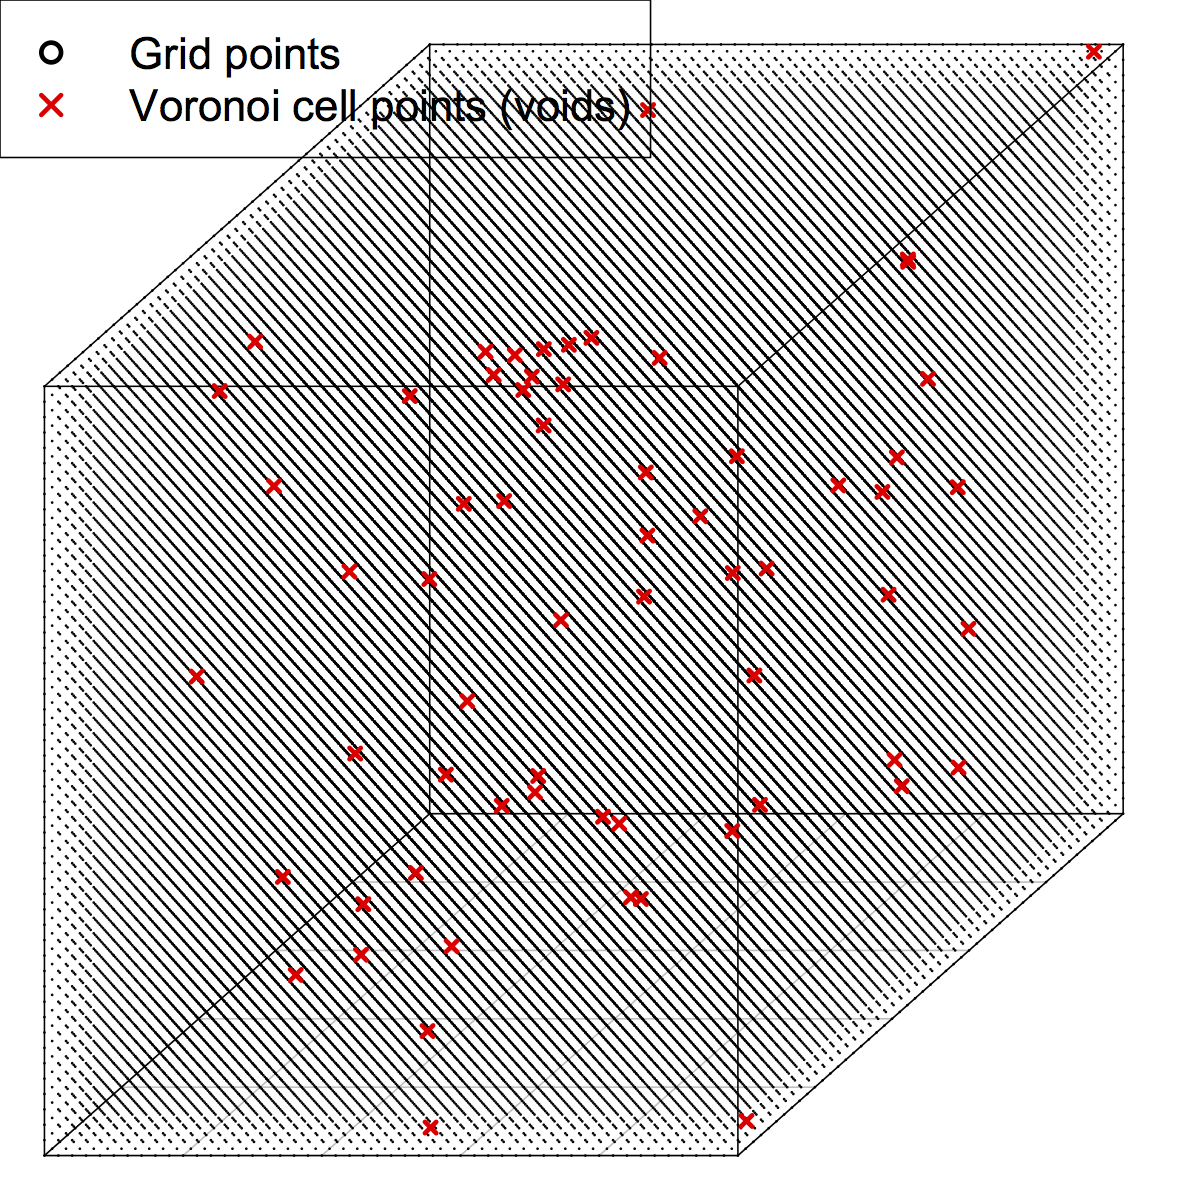
\includegraphics[height=2.25in]{fig_vf_grid.png}
        \caption{Grid and selected voids} \label{subfig:grid}
    \end{subfigure}%
    ~
    \begin{subfigure}[t]{0.5\textwidth}
        \centering
        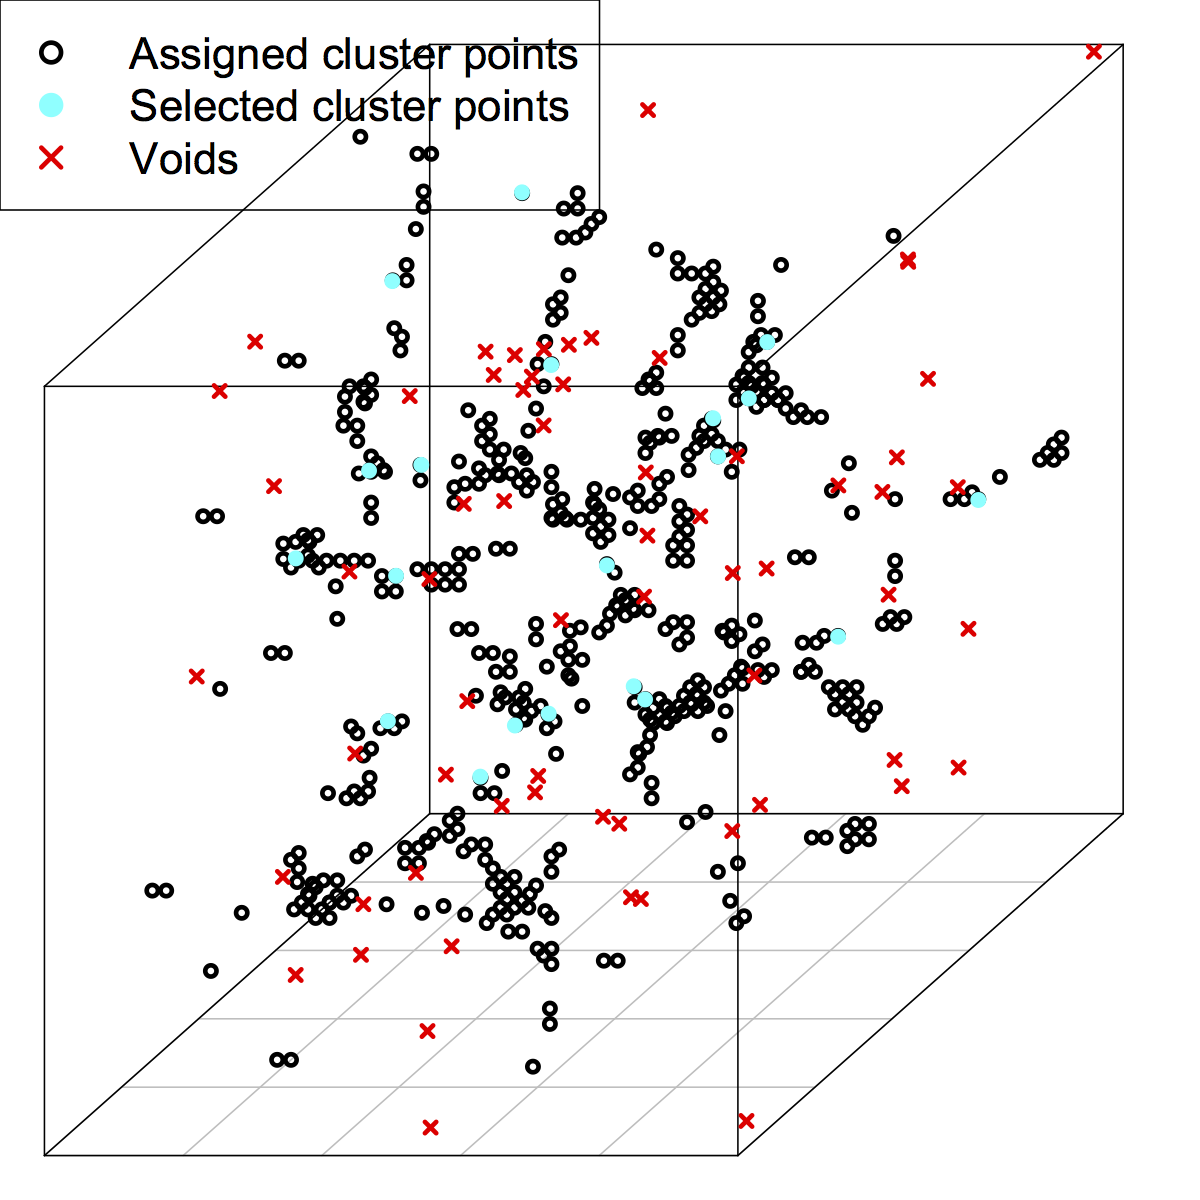
\includegraphics[height=2.25in]{fig_vf_cluster.png}
        \caption{Cluster points} \label{subfig:cluster}
    \end{subfigure} \\

     \begin{subfigure}[t]{0.5\textwidth}
      \centering
    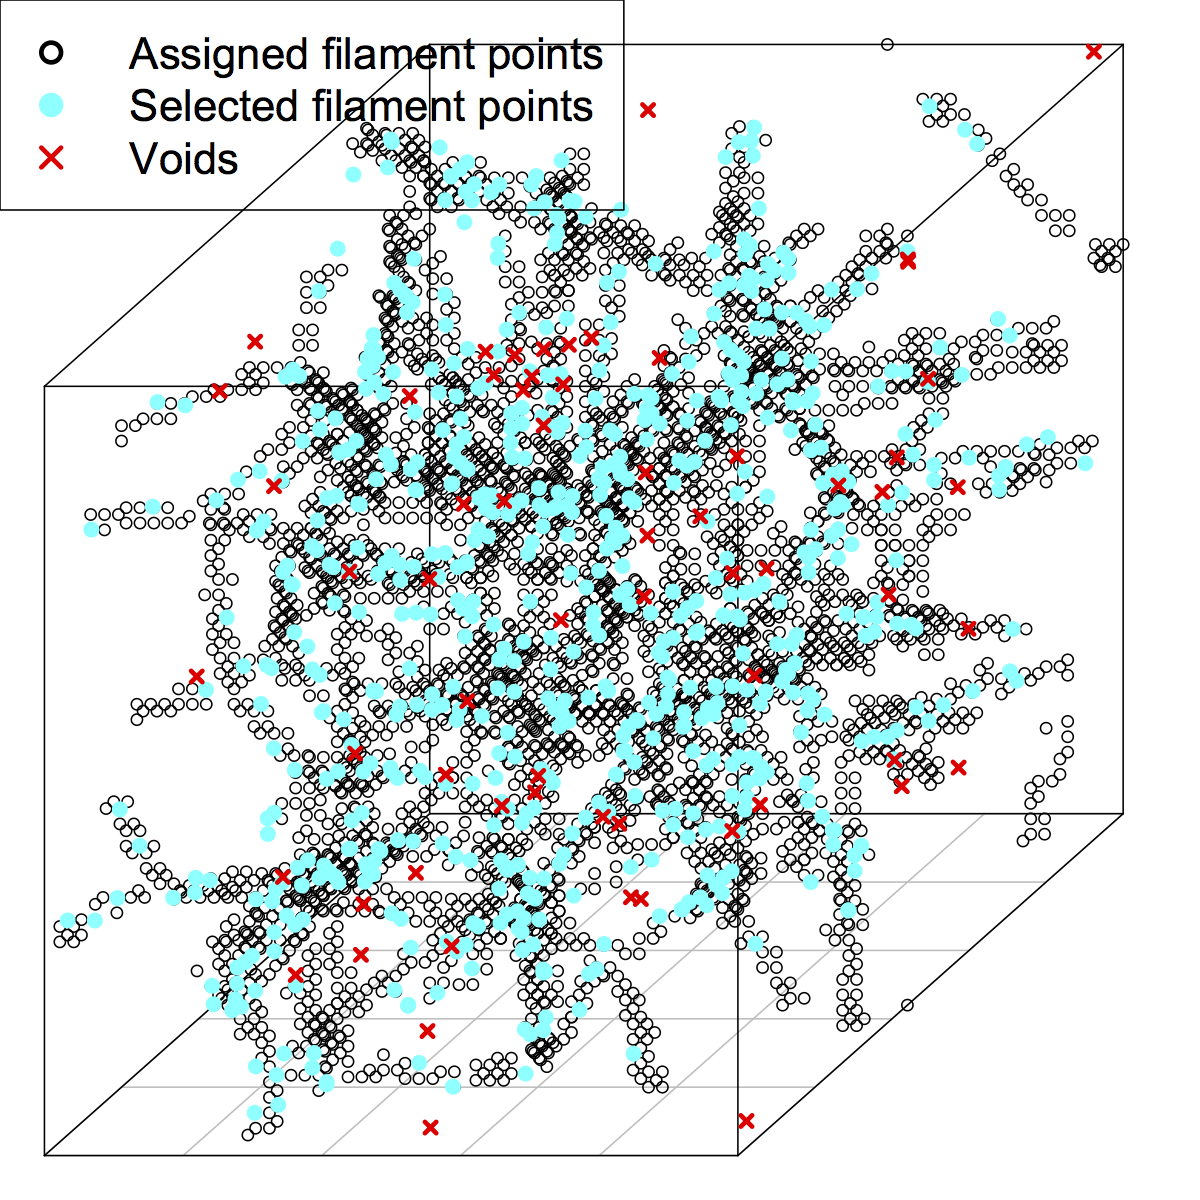
\includegraphics[height=2.25in]{fig_vf_fil.png}
     \caption{Filament points} \label{subfig:fil}
    \end{subfigure}%
    ~
    \begin{subfigure}[t]{0.5\textwidth}
        \centering
        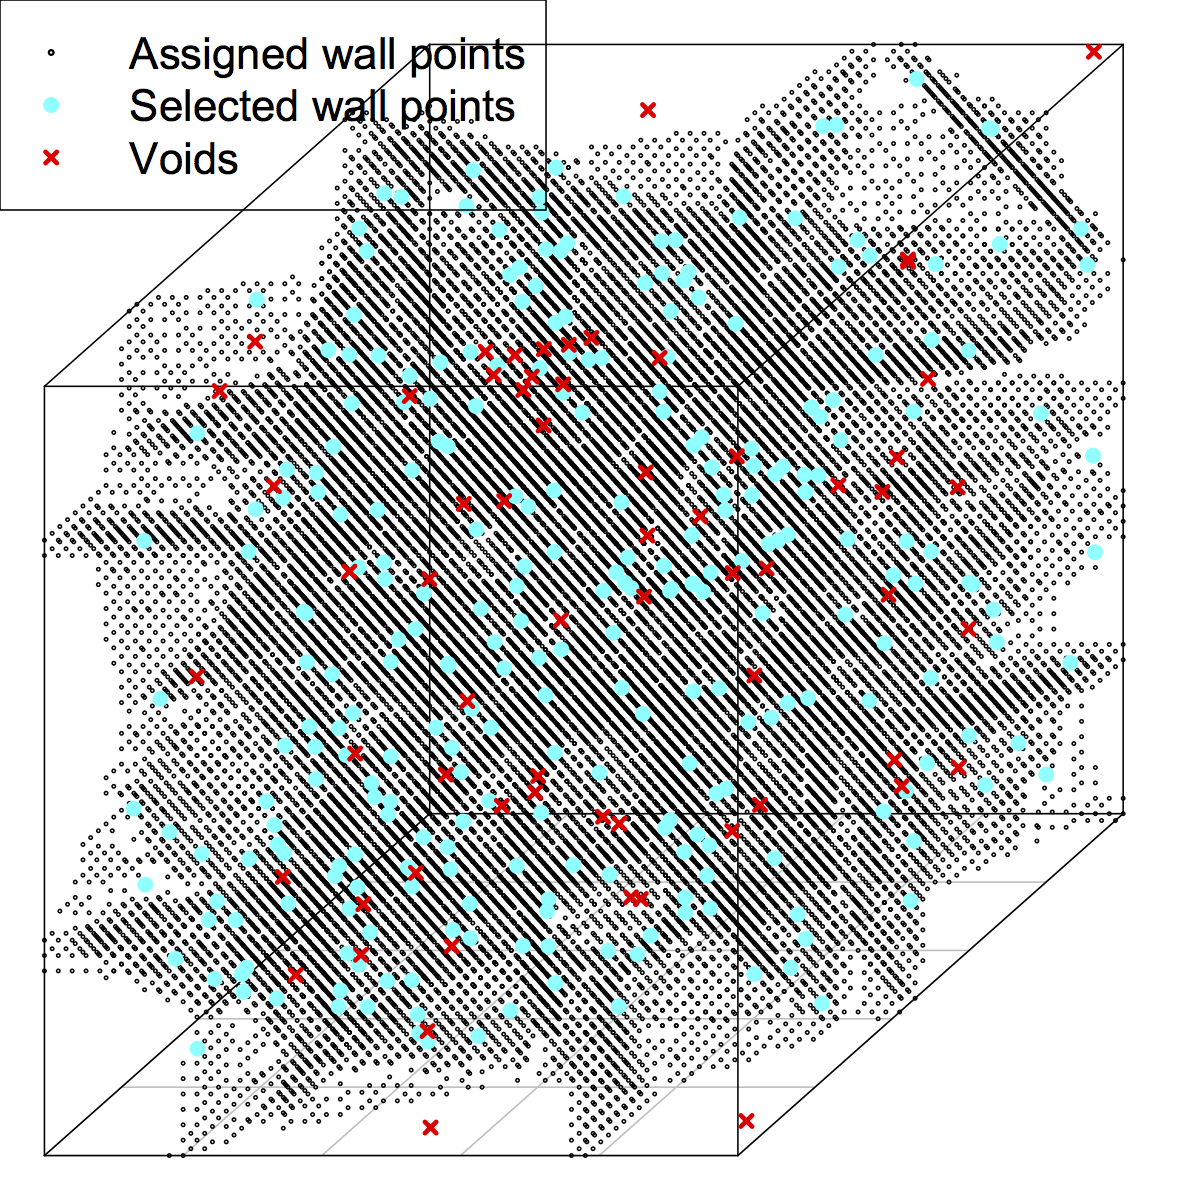
\includegraphics[height=2.25in]{fig_vf_wall.png}
        \caption{Wall points} \label{subfig:wall}
    \end{subfigure}
    \caption{Simulation model construction.  (a) A grid is defined and points are randomly selected to define the Voronoi tesselation - the Voronoi cells are the voids.  (b) - (d) Based on the location of the voids and the grid, points are defined to be cluster points, filament points or wall points - these are the empty black circles.  Based on the values assigned from Table~\ref{table:voronoisettings}, a number of points are randomly selected from the assigned points to be in the dataset.} \label{fig:vf}
\end{figure*}

% introduced the Voronoi foam as a packing of polyhedral units with walls representing pancakes, edges representing filaments, and vertices representing clusters in the galaxy. Icke showed that the Voronoi foam is an appropriate model for a 10-500 Mpc scale Universe with pressure-free Newtonian gravitational collapse. Statistical study showed that the spatial two-point correlation of Voronoi foams has a power law behavior with close to identical amplitude and slope as that of actual Abell clusters \citep{vanvoronoi}.
% A Voronoi foam model, is generated from a tessellation, where the edges of each cell represent filaments and the faces of the cell, enclosed voids. Given a plane with fixed size, such a tessellation partitions the plane into cellular regions with nuclei. Every cell territory is defined as the set of points equal or closer to that cell's nuclei than any other. To produce a simulation in polynomial time, each point in the plane is compared to the $k$ closest nuclei using a nearest neighbor algorithm where $k$ is chosen to be a small integer. Gaussian noise is added to perturb the plane and inject randomness. Because the nuclei number and the plane size are variable, the points in the simulation representing filaments, clusters, and walls are variable as well. By choosing a reasonable percentage of filaments and related structures, Voronoi simulations are to approximate the topology and LSS of true simulations of the observable Universe. By varying these percentages and repeating simulations, one can quickly generate a large, labeled data sets for hypothesis testing. Our interest primarily was gauging the effect of changing the percent filament in the Voronoi tessellation on the ability of the hypothesis tests to distinguish two foam models sampled from different tessellations.


Examples of three separate Voronoi foam models with percFil 0.1, 0.5, 0.9 are displayed in \figref{fig:percfilexample} along with their corresponding persistence diagrams. One can see that the as the percFil increases, the web-like structure becomes more pronounced, changing the distribution of topological features.

\begin{center}
  \begin{figure}[htp!]
    \centering
    \begin{subfigure}{.32\textwidth}
      \centering
      \caption{PercFil 0.1 (Voronoi)}
      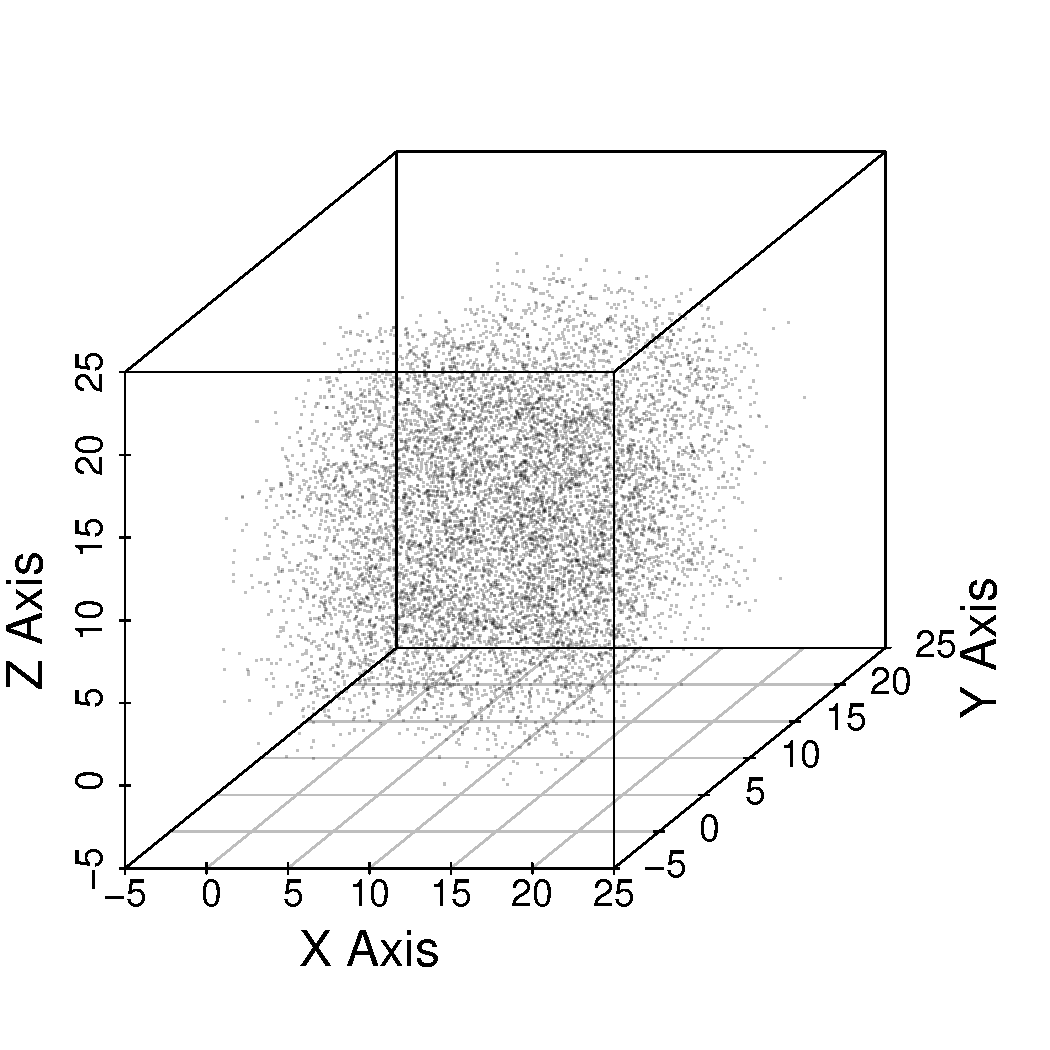
\includegraphics[width=0.6\linewidth]{figure_7_plot_pf_0_1.pdf}
      \label{fig:percfil01voronoi}
    \end{subfigure}
      \begin{subfigure}{.32\textwidth}
      \centering
      \caption{PercFil 0.5 (Voronoi)}
      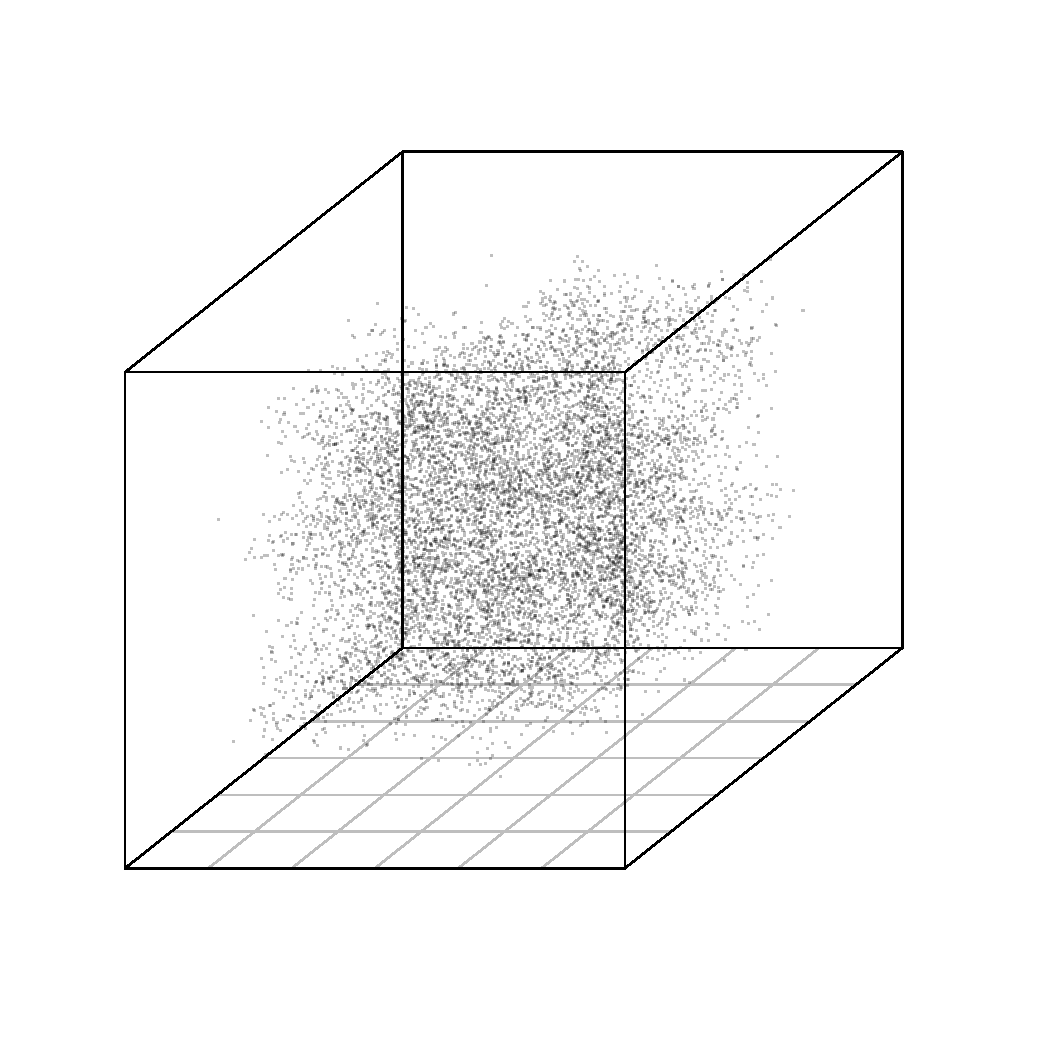
\includegraphics[width=0.6\linewidth]{figure_7_plot_pf_0_5.pdf}
      \label{fig:percfil09voronoi}
    \end{subfigure}
      \begin{subfigure}{.32\textwidth}
      \centering
      \caption{PercFil 0.9 (Voronoi)}
      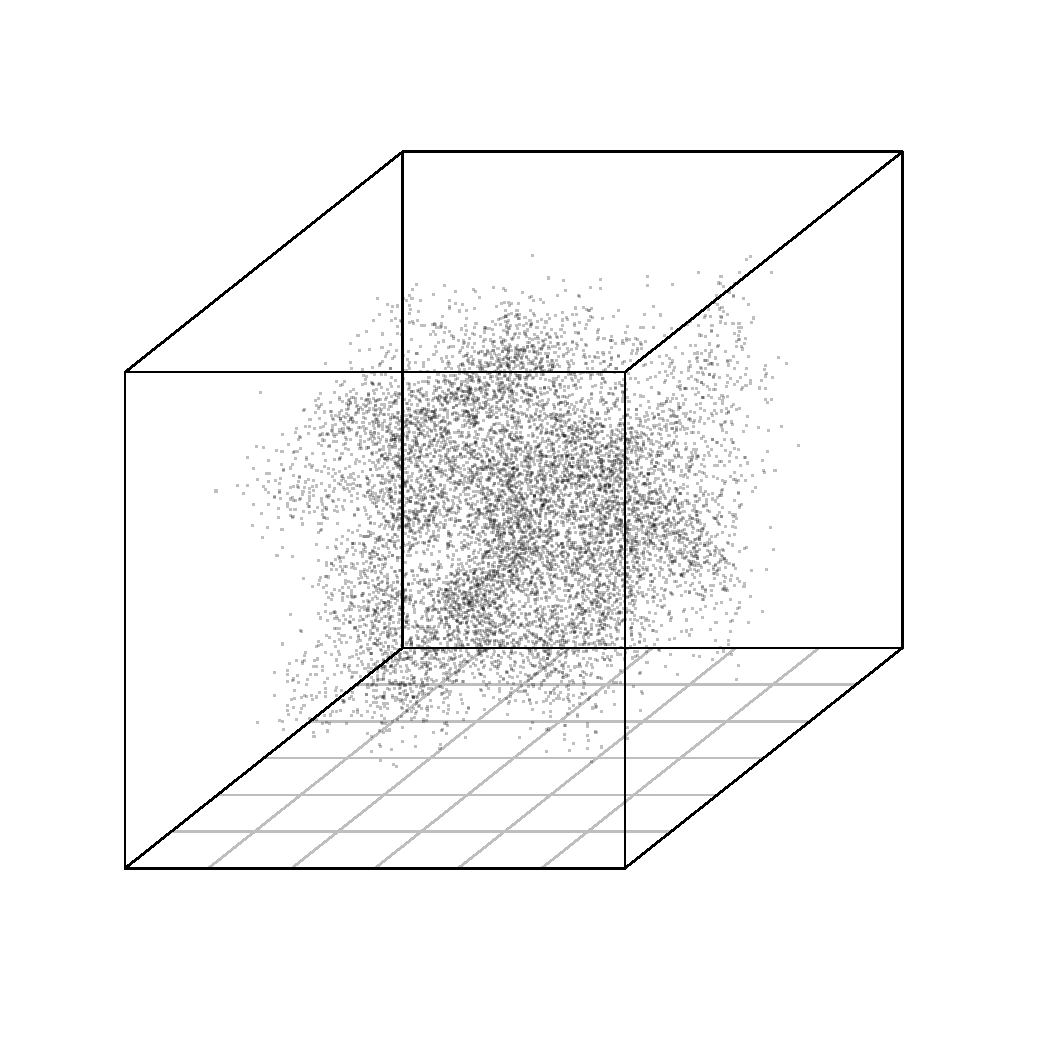
\includegraphics[width=0.6\linewidth]{figure_7_plot_pf_0_9.pdf}
      \label{fig:percfil09voronoi}
    \end{subfigure}
      \begin{subfigure}{.32\textwidth}
      \centering
      \caption{PercFil 0.1 (PD)}
      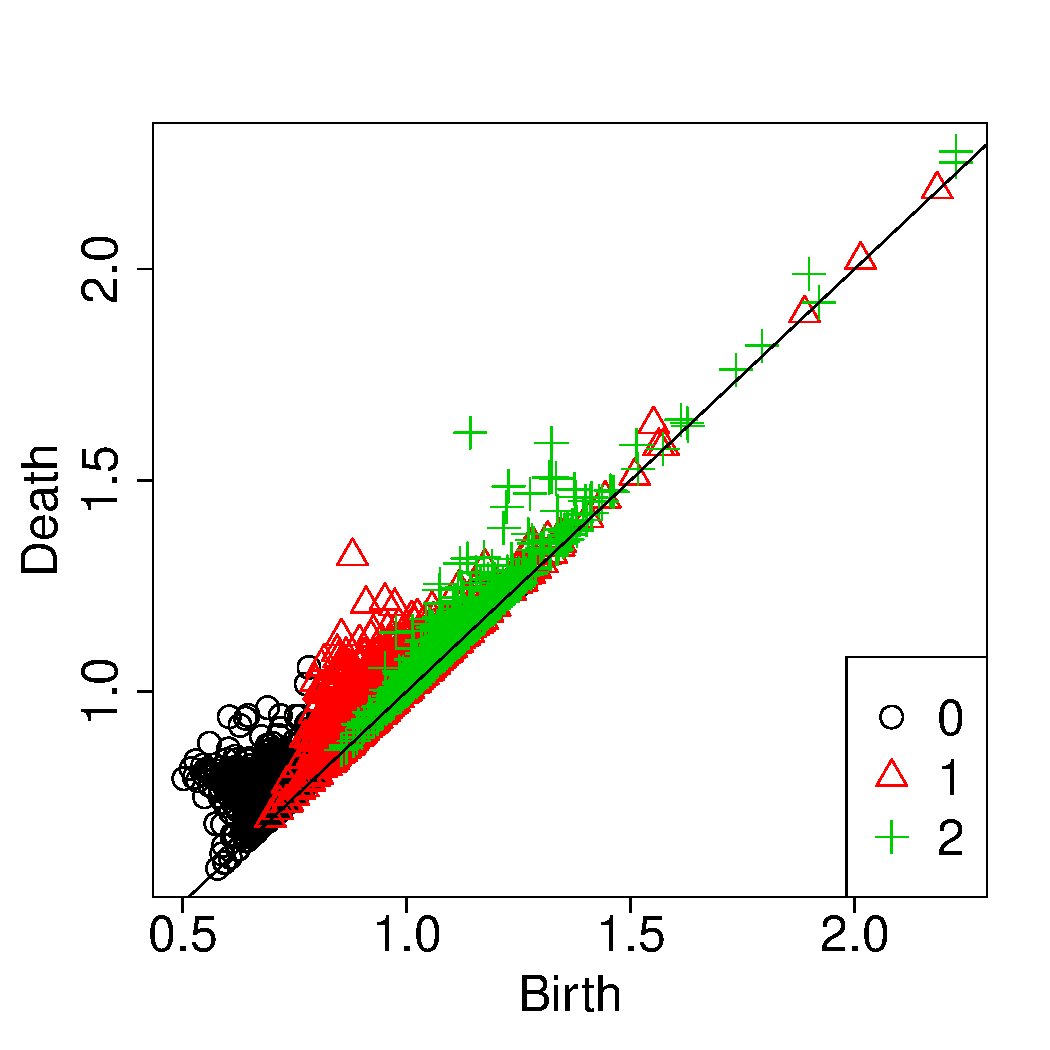
\includegraphics[width=0.6\linewidth]{figure_7_pd_0_1.pdf}
      \label{fig:percfil01pd}
    \end{subfigure}
      \begin{subfigure}{.32\textwidth}
      \centering
      \caption{PercFil 0.5 (PD)}
      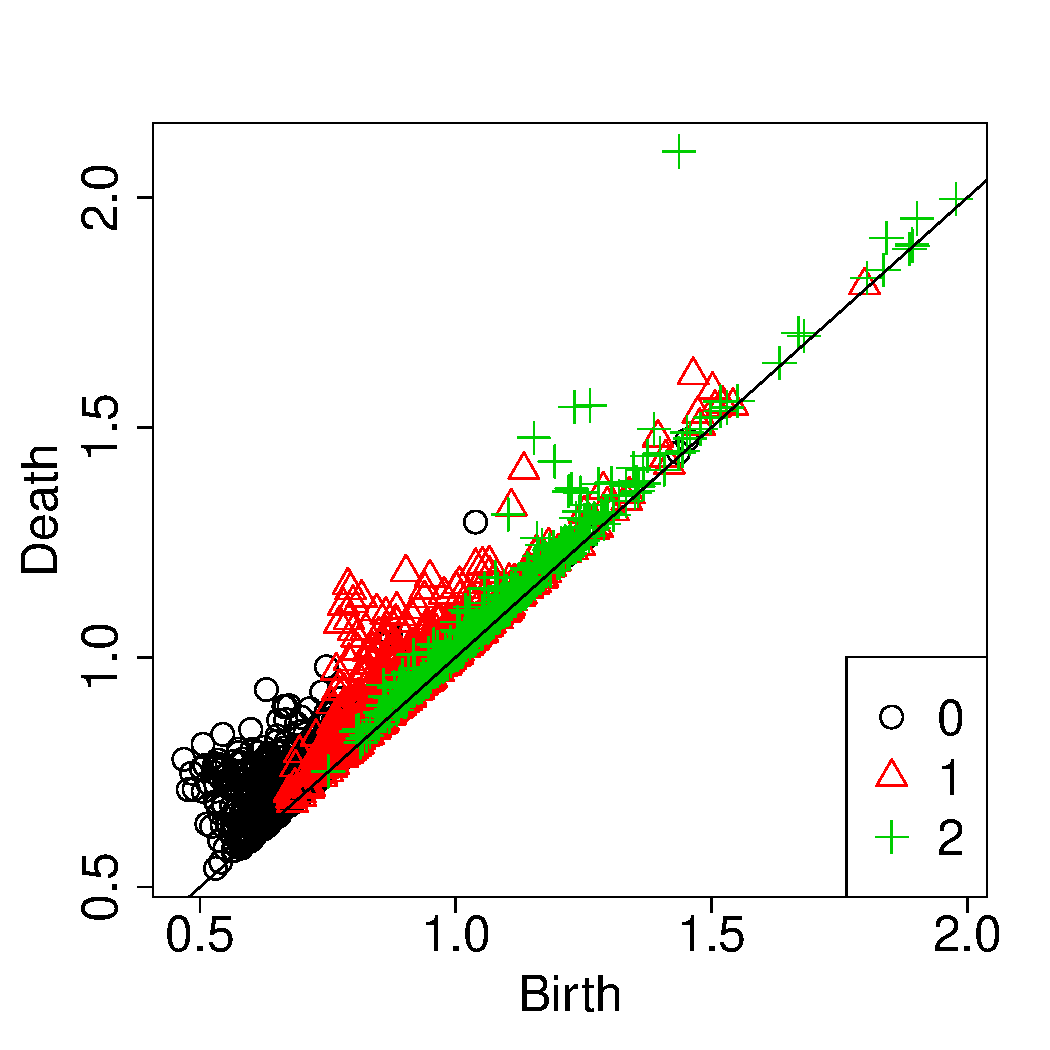
\includegraphics[width=0.6\linewidth]{figure_7_pd_0_5.pdf}
      \label{fig:percfil09pd}
    \end{subfigure}
      \begin{subfigure}{.32\textwidth}
      \centering
      \caption{PercFil 0.9 (PD)}
      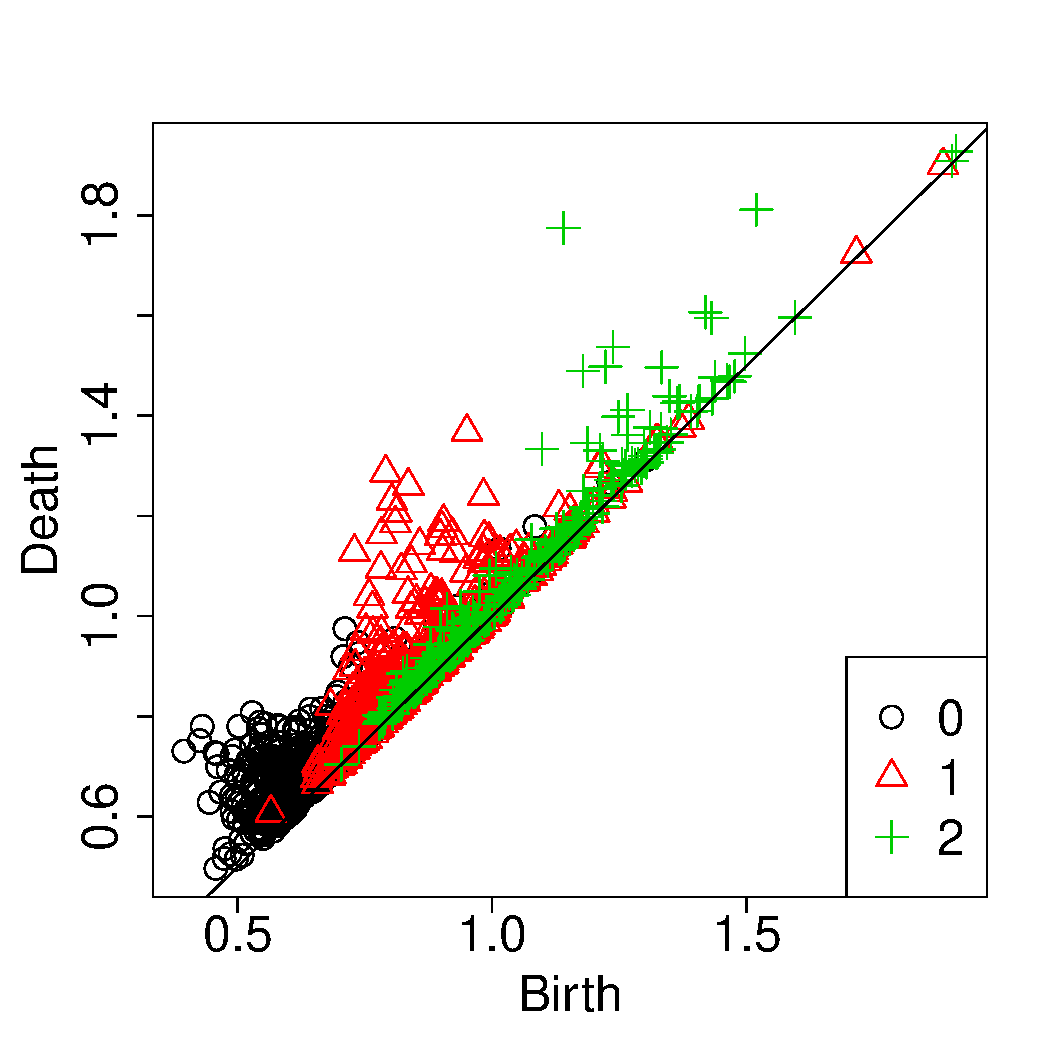
\includegraphics[width=0.6\linewidth]{figure_7_pd_0_9.pdf}
      \label{fig:percfil09pd}
    \end{subfigure}
      \caption{Three examples of Voronoi foam simulations and their corresponding persistence diagrams using 3 different filament densities. As the percent filament increases, the point clouds tend to co-agulate into dense and sparse regions; the persistence diagrams also form more features with longer lifespans. All other parameters used the generate the Voronoi foams are defined based on Table~\ref{table:voronoisettings}.}
      \label{fig:percfilexample}
  \end{figure}
\end{center}

\subsection{Simulation Study Results}
\label{sec:results1}
The Voronoi foams used in this paper were generated under $1.25 \times  10^{5}$ box volume, $0.1$ resolution, $1 \times  10^{4}$ points, $64$ cells (voids), 0.02 percClust, and $[0.1, 0.3]$ percFil and $[0.68, 0.88]$ percWall. Persistent diagrams are generated using distance-to-measure (DTM) with a $0.01$ tuning parameter. The diagrams are preprocessed to remove the known 0-dimensional artifact, a vestigial $H_{0}$ element with birth time of 0 and a death time of $\infty$ (with exception to the EC test in which the artifact is preserved). The hypothesis tests were performed on 100 independent iterations of 15 independent realizations from each of the two populations. The 15 independent datasets are each generated using a percFil setting from 0.1 to 0.3 (0.05 step size); we also include a control model per iteration with a percFil of 0.1. (Hence 5 sets of 15 datasets, repeated 100 times.) Using the proposed hypothesis tests, each of the variable models will be compared to the control. Given the data drawn from a model with percFil $p$, each of the proposed test statistics are used to compute a p-value for the test $H_0: \mathcal
P^{(1)} = \mathcal P^{(2)}$ vs. $H_1: \mathcal P^{(1)} \neq \mathcal P^{(2)}$,
based on two samples of persistence diagrams, $\{\mathcal
P_1^{(1)}, \ldots, \mathcal P_{15}^{(1)}\}$ drawn from the model with percFil = 0.1, and $\{\mathcal P_1^{(2)}, \ldots,
\mathcal P_{15}^{(2)}\}$ drawn from the model with percFil = $p$, $p = 0.1, 0.15, \ldots, 0.3$.
(Recall that $\mathcal P^{(1)}$ and $\mathcal P^{(2)}$ are the true underlying
distributions of persistence diagrams for group 1 and 2, respectively.)
Similar tests were also completed against a control model with 0.3 percFil, and agreeable results were found. The simulation study results are displayed in \figref{fig:linesUnnormApp}, which shows the median p-values along with a (min, max) confidence interval across the 100 iterations of the following test statistics: (i) Euler-based tests, (ii) Silhouette-based tests, (iii) Kernel-based tests, (iv) Weighted Kernel-based tests, and (v) Correlation-based tests.

\begin{figure}[htp!]
  \centering
  \begin{subfigure}{.8\textwidth}
    \centering
    \caption{EC Tests}
    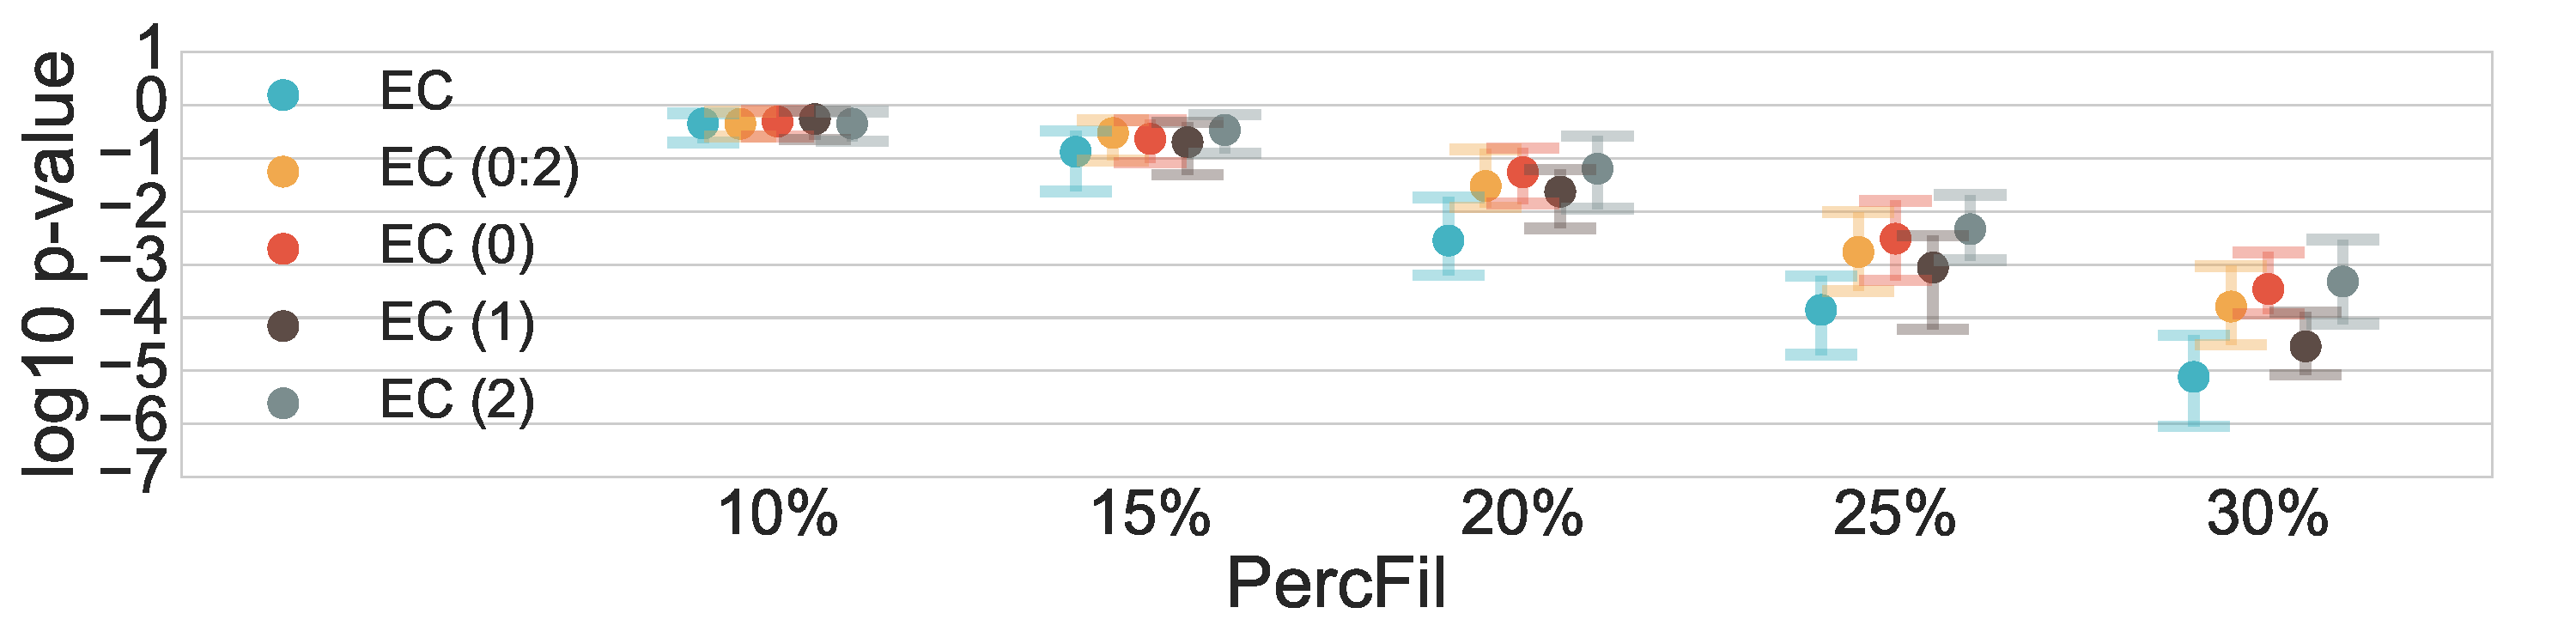
\includegraphics[width=\linewidth]{figure_8_euler_group.pdf}
    \label{fig:sub_euler}
  \end{subfigure}
  \begin{subfigure}{.8\textwidth}
    \centering
    \caption{EC Tests (Normed)}
    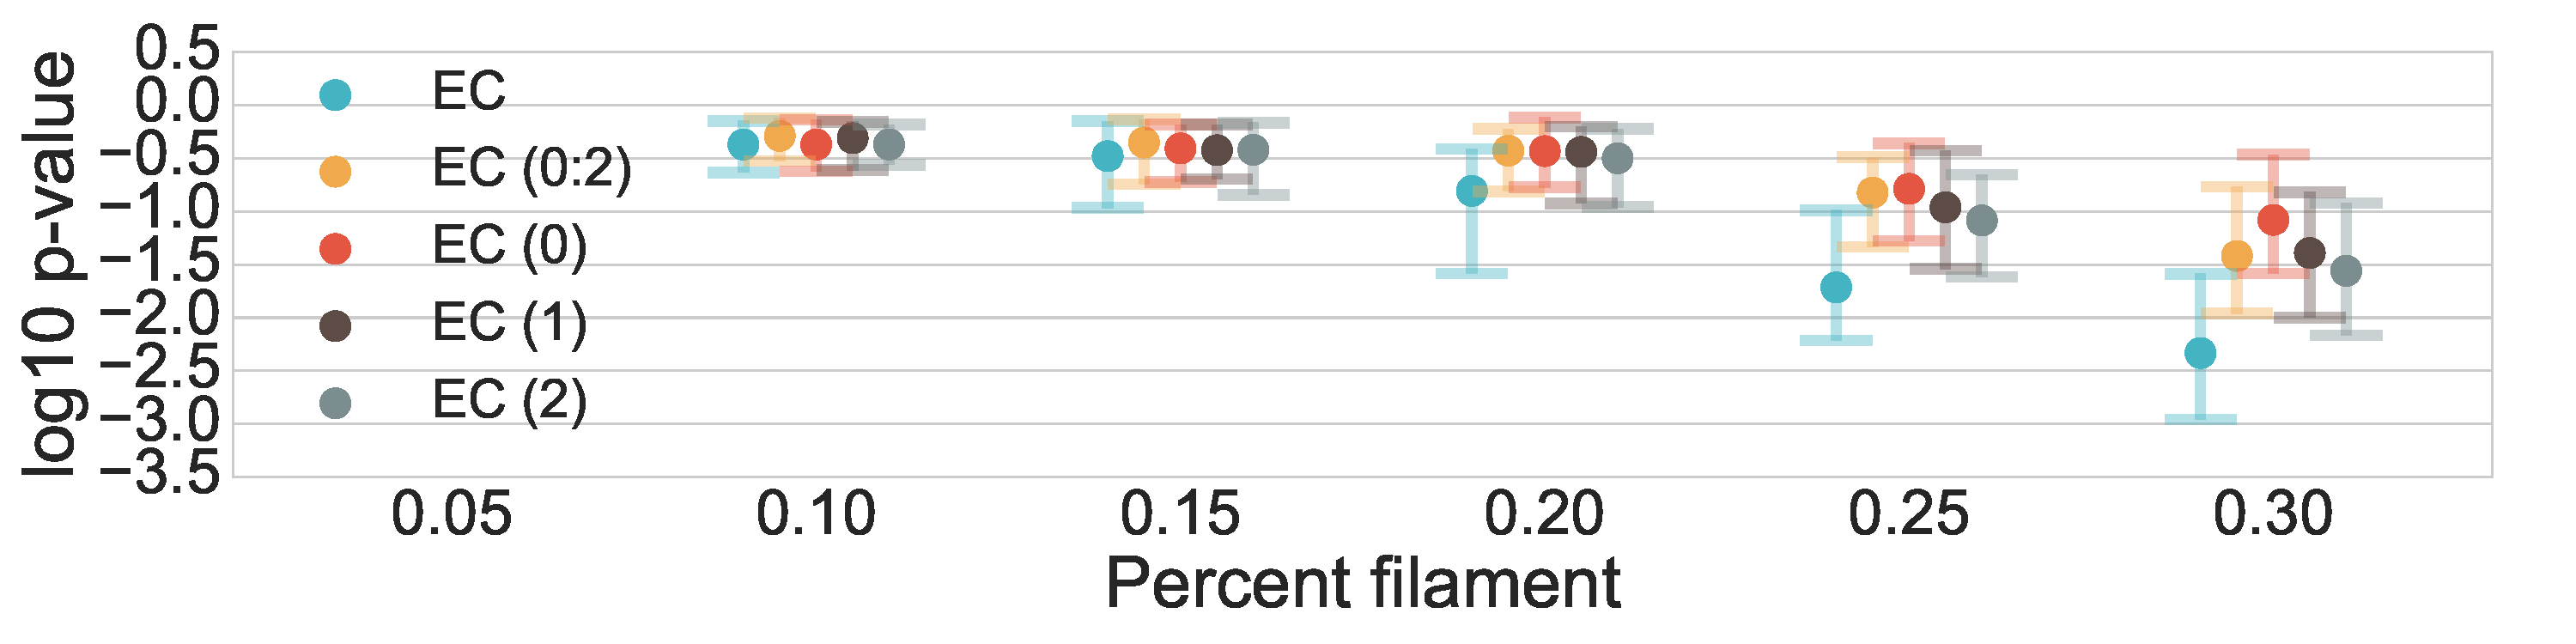
\includegraphics[width=\linewidth]{figure_8_euler_group_normed.pdf}
    \label{fig:sub_euler_normed}
  \end{subfigure}
\caption{P-values from a suite of EC tests. X-axis represents a percent filament (0.1 to 0.3) being compared to a baseline of 0.1; Y-axis shows the p-values in $\textup{1og}_{10}$ space. The lines plot the median $\log_{10}$ p-value and error bars show the 25th and 75th percentile p-values of the 100 iterations. \figref{fig:sub_euler_normed} is identical to \figref{fig:sub_euler} with the exception of standardizing the persistence diagrams prior to testing. }
\label{fig:sub_euler_results}
\end{figure}

\begin{figure}[htp!]
  \centering
  \begin{subfigure}{.8\textwidth}
    \centering
    \caption{SIL Tests}
    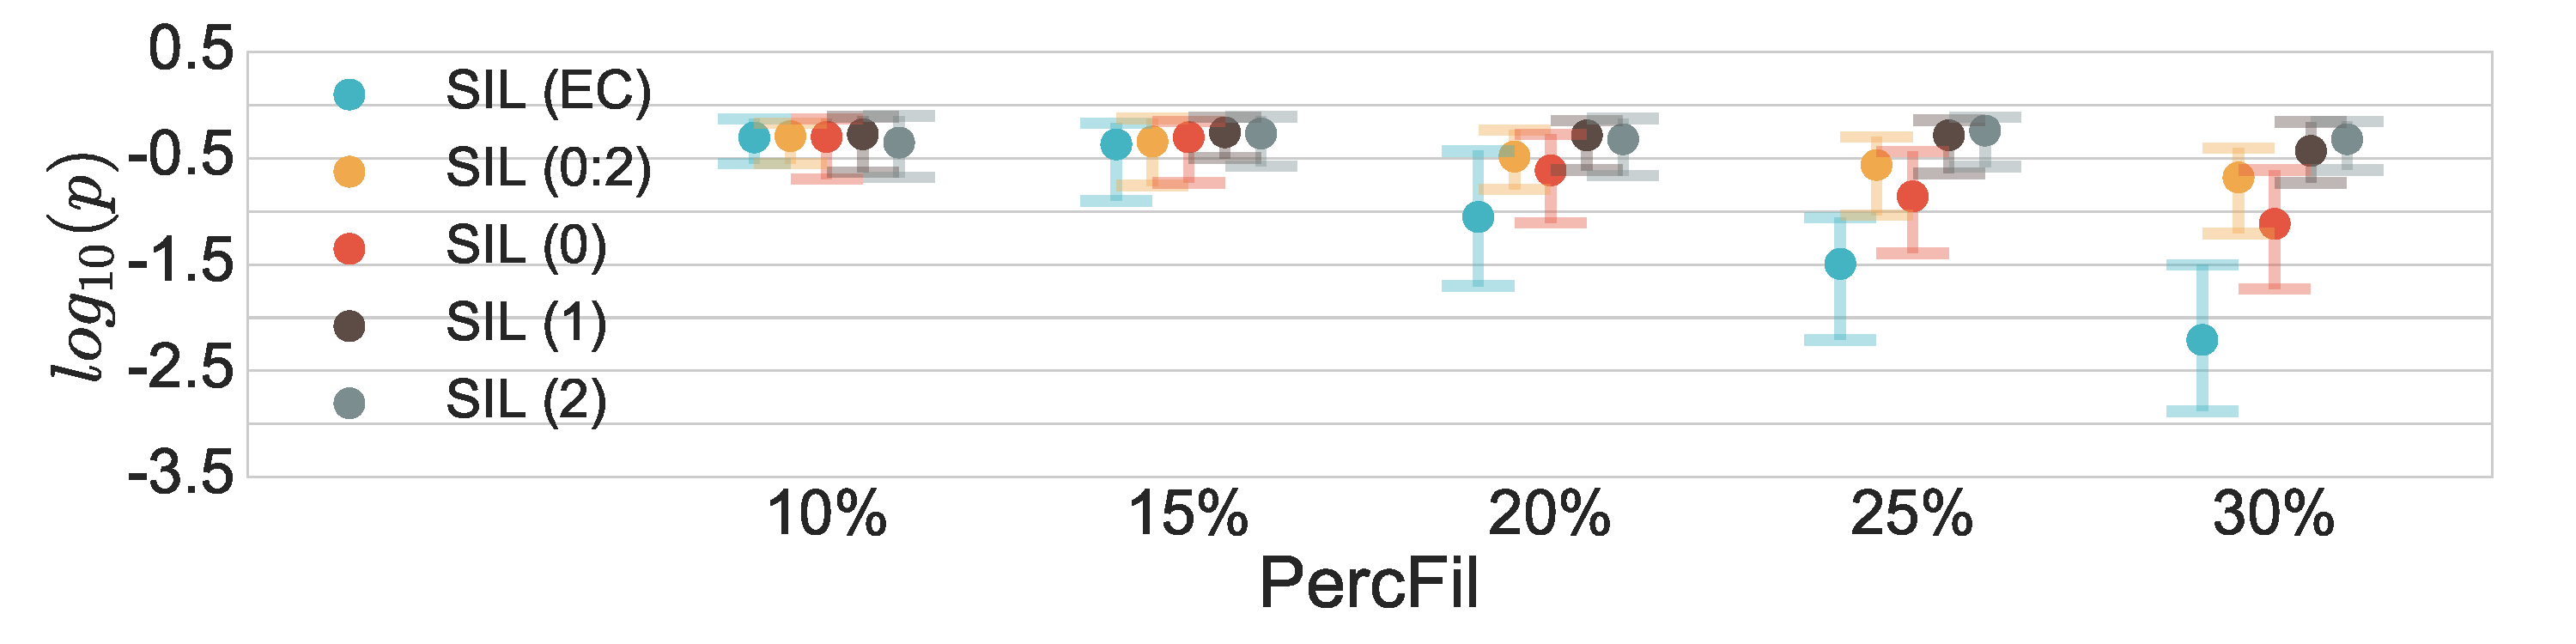
\includegraphics[width=\linewidth]{figure_8_silhouette_group.pdf}
    \label{fig:sub_silh}
  \end{subfigure}
  \begin{subfigure}{.8\textwidth}
    \centering
    \caption{SIL Tests (Normed)}
    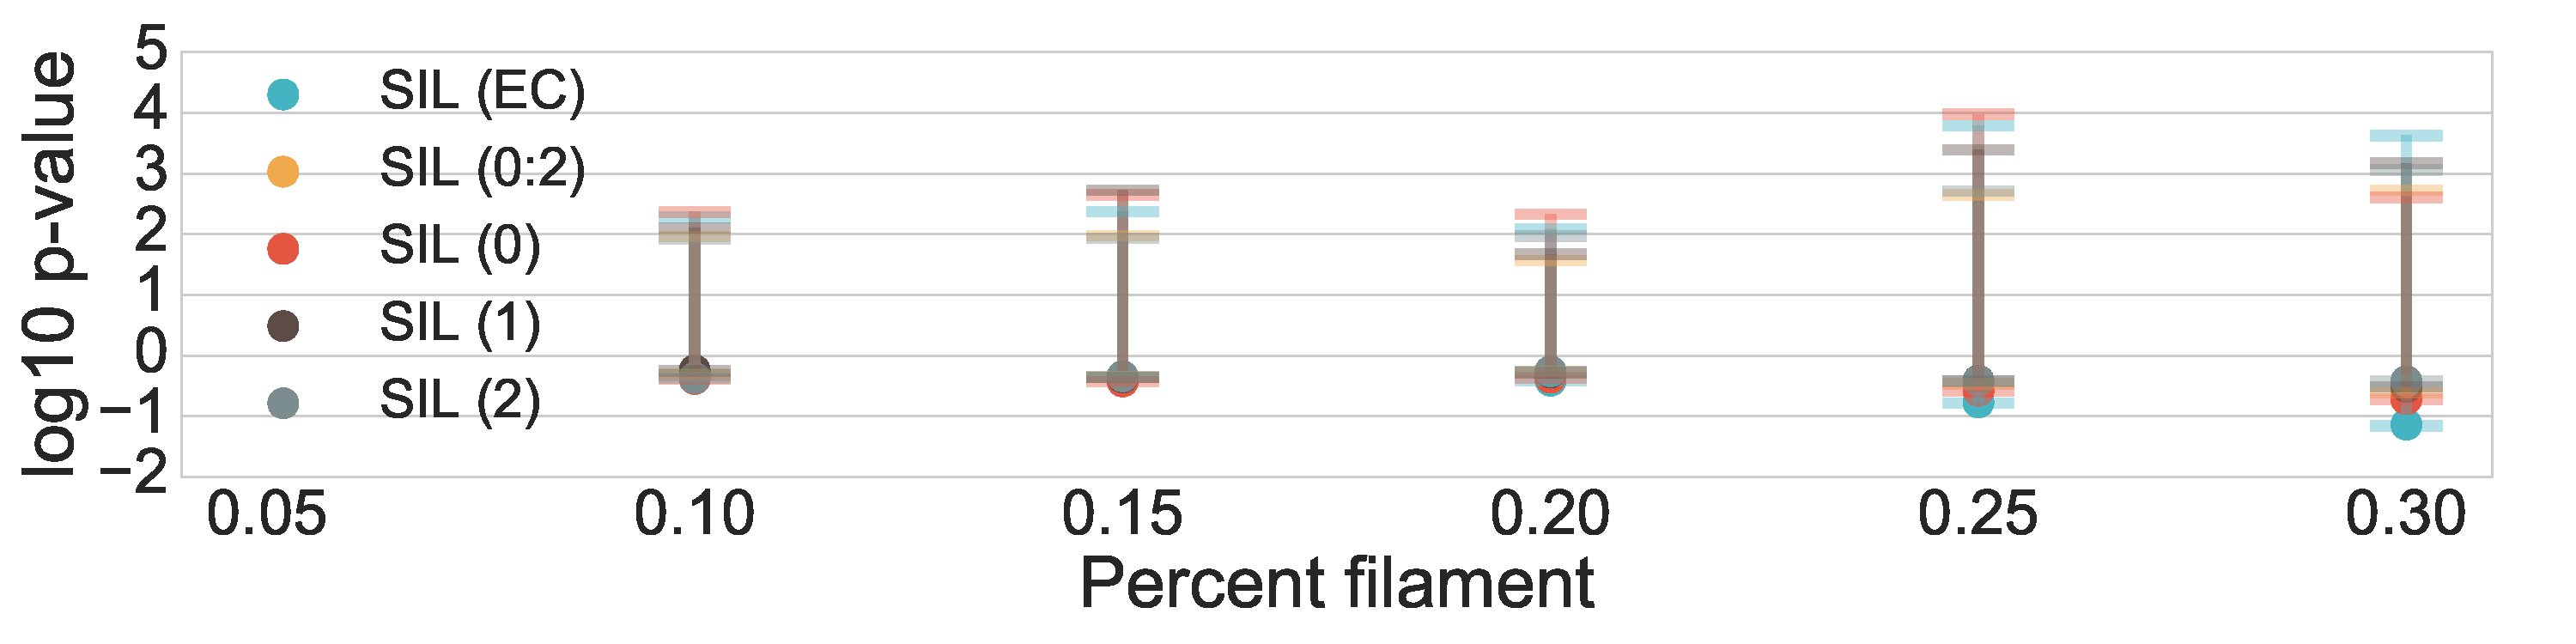
\includegraphics[width=\linewidth]{figure_8_silhouette_group_normed.pdf}
    \label{fig:sub_silh_normed}
  \end{subfigure}
\label{fig:sub_silh_results}
\caption{P-values from a suite of SIL tests.}
\end{figure}

\begin{figure}[htp!]
  \centering
  \begin{subfigure}{.8\textwidth}
    \centering
    \caption{IK Tests}
    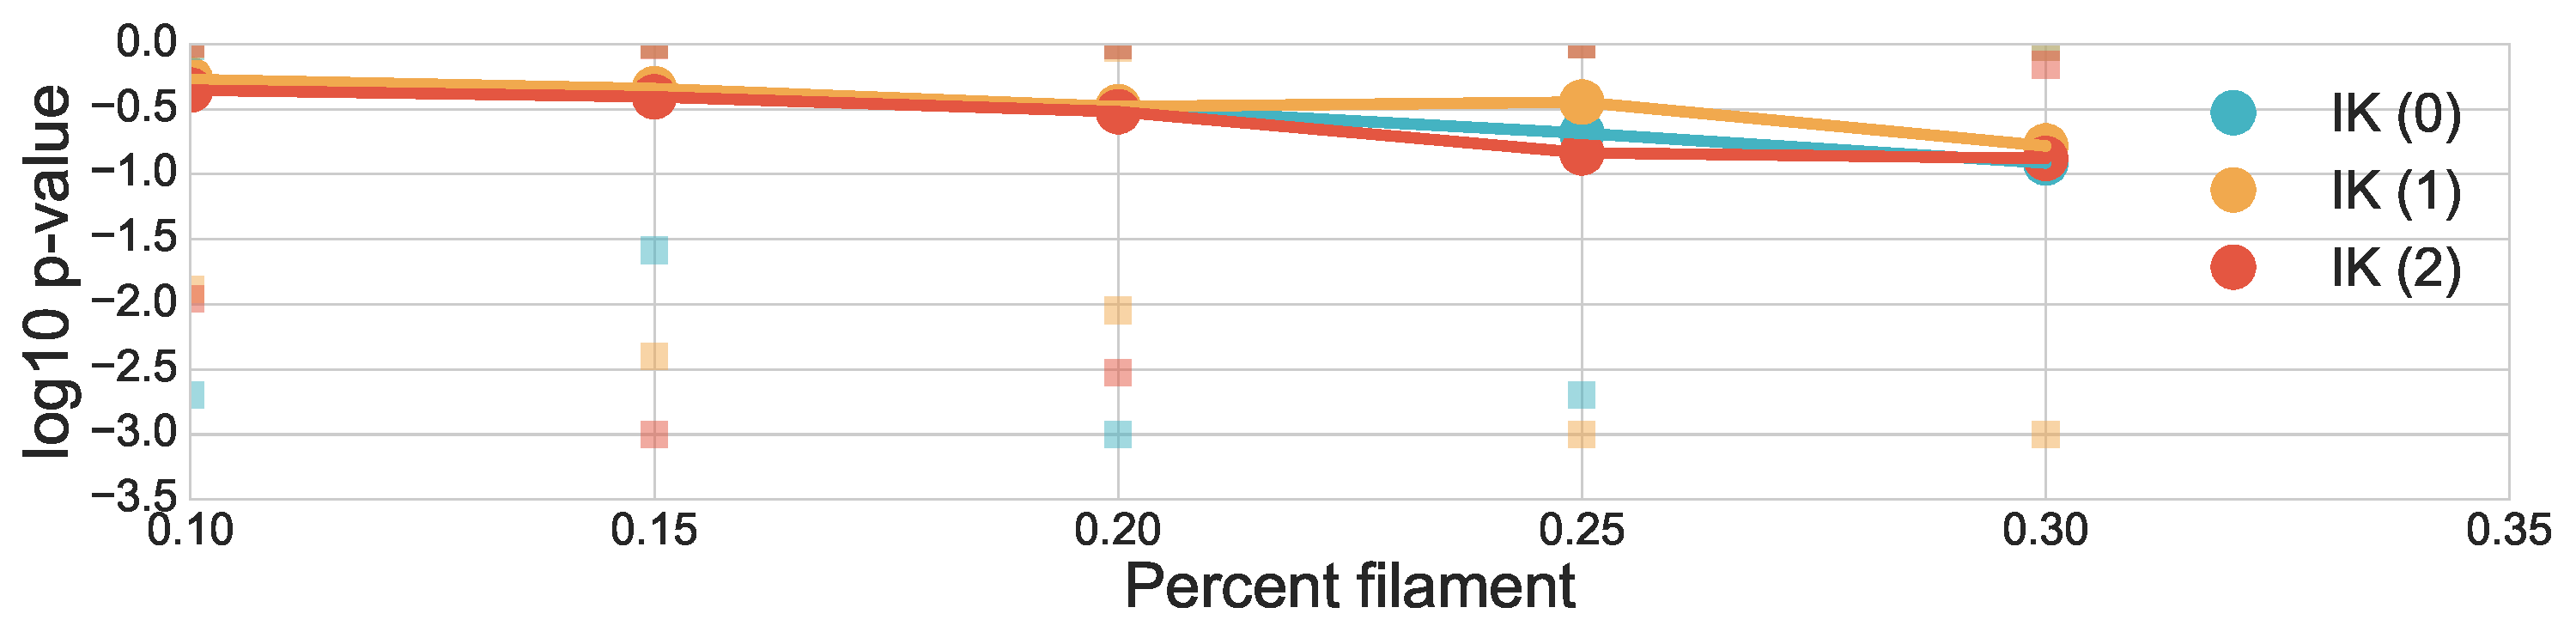
\includegraphics[width=\linewidth]{figure_8_contour_group.pdf}
    \label{fig:sub_contour}
  \end{subfigure}
  \begin{subfigure}{.8\textwidth}
    \centering
    \caption{IK Tests (Normed)}
    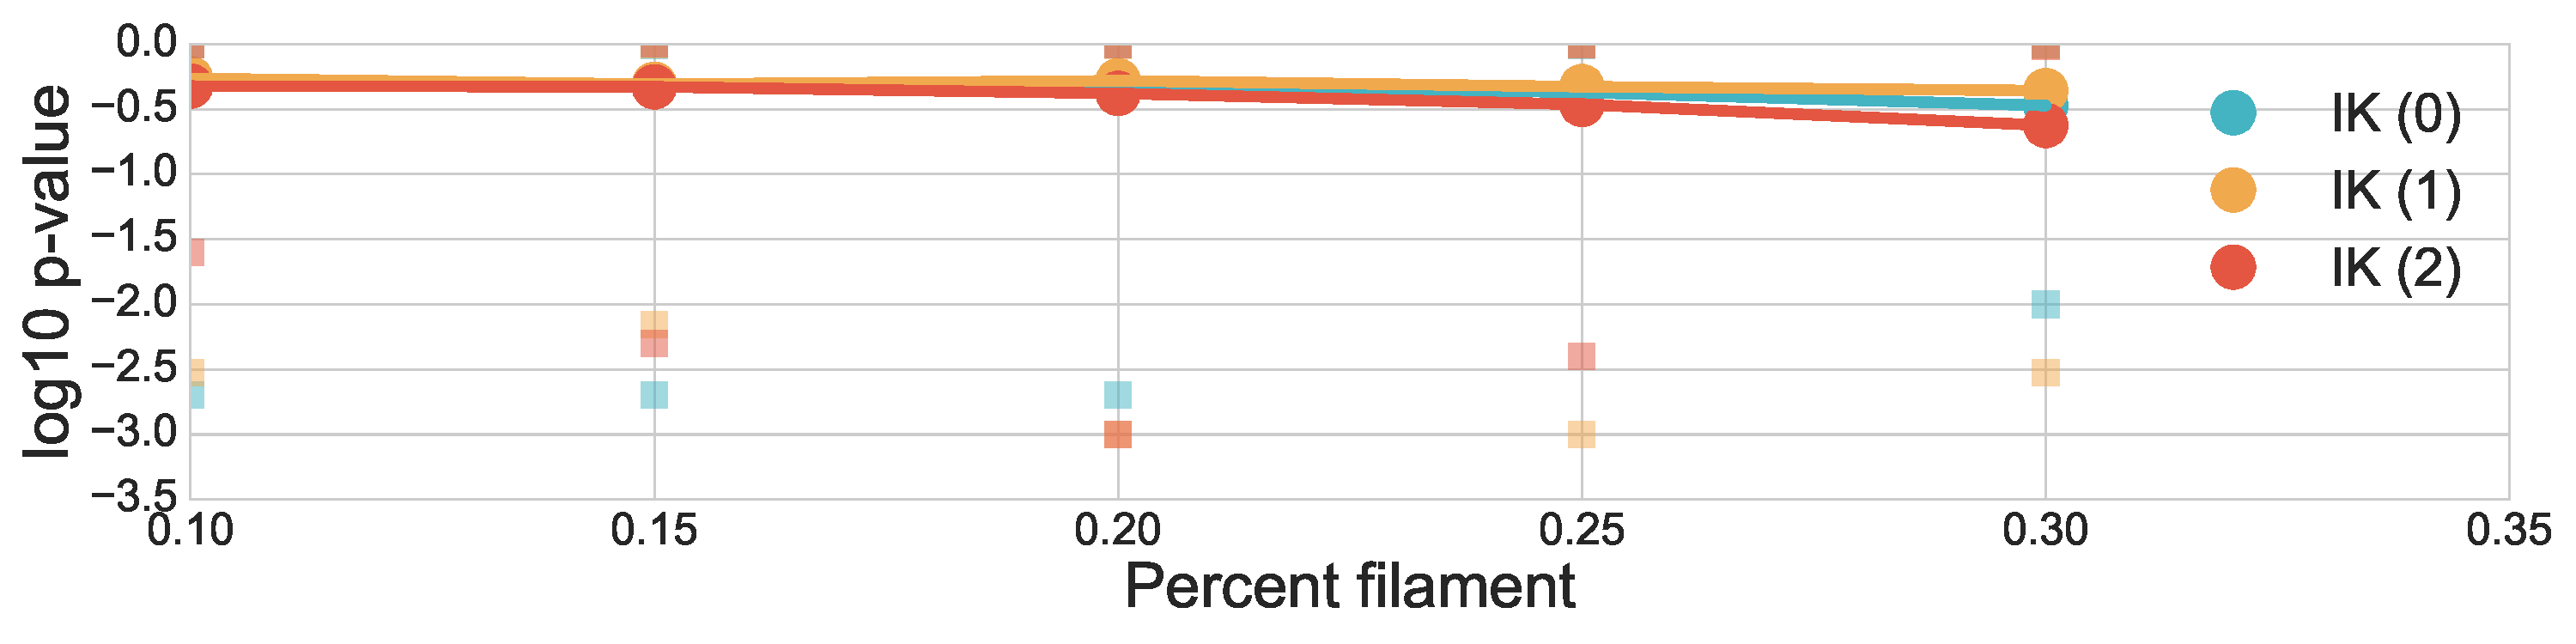
\includegraphics[width=\linewidth]{figure_8_contour_group_normed.pdf}
    \label{fig:sub_contour_normed}
  \end{subfigure}
\label{fig:sub_contour_results}
\caption{P-values from a suite of IK tests.}
\end{figure}

\begin{figure}[htp!]
  \centering
  \begin{subfigure}{.8\textwidth}
    \centering
    \caption{WIK/PI Tests}
    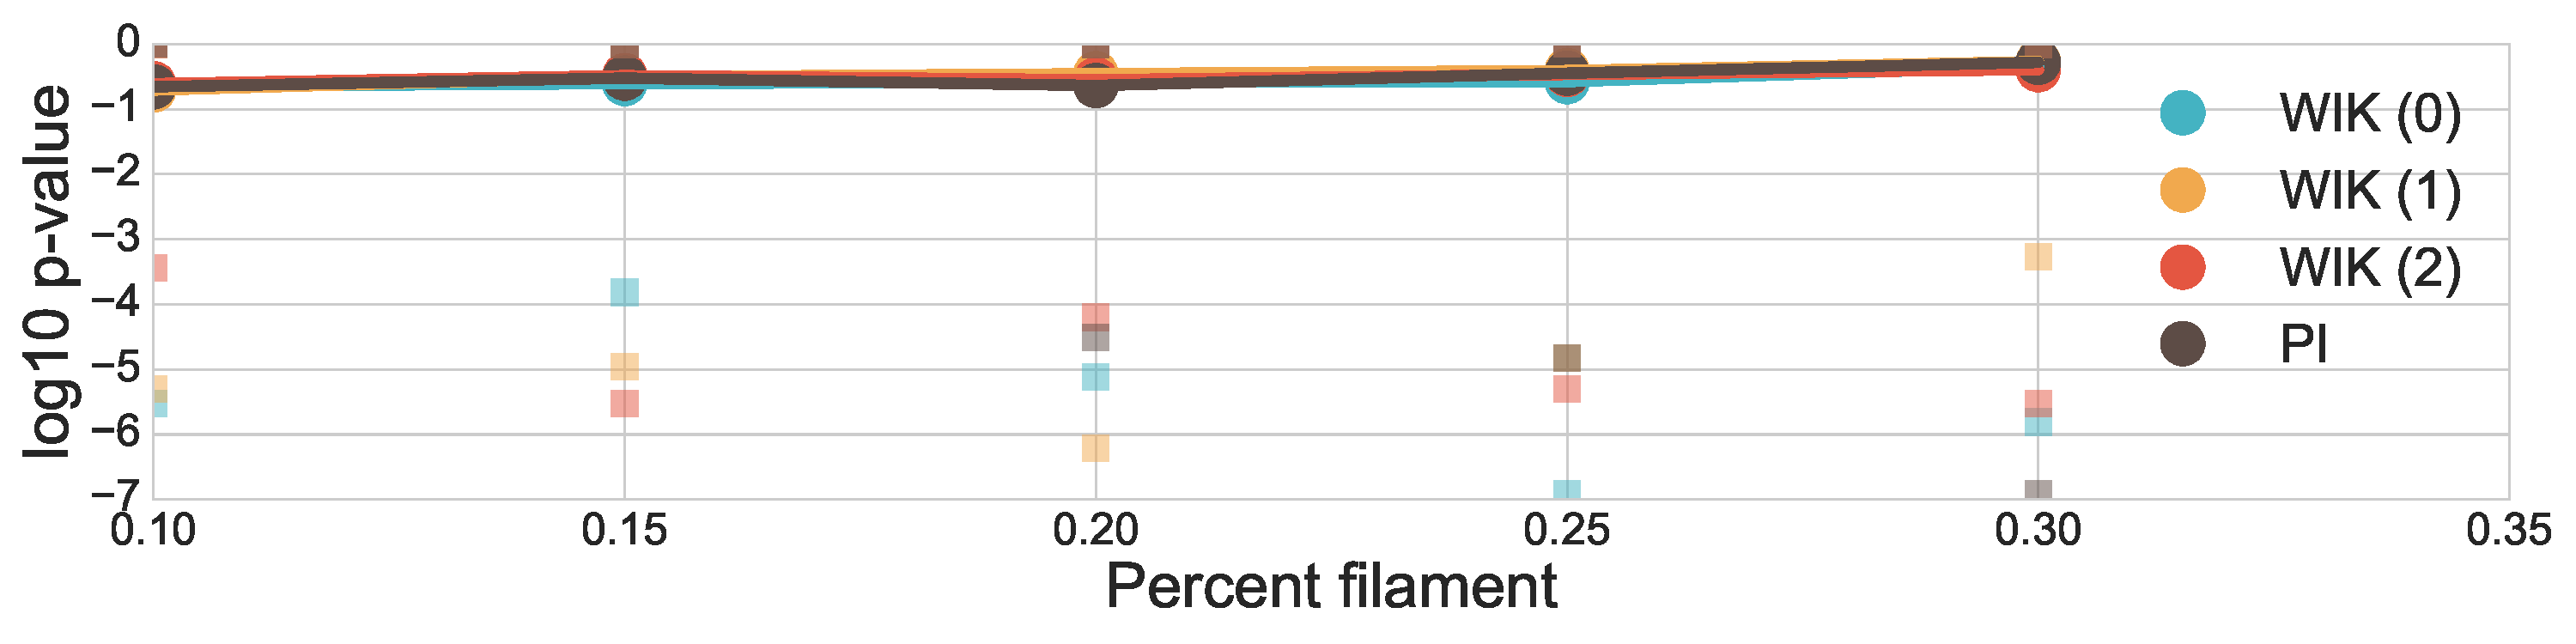
\includegraphics[width=\linewidth]{figure_8_weighted_contour_group.pdf}
    \label{fig:sub_weight}
  \end{subfigure}
  \begin{subfigure}{.8\textwidth}
    \centering
    \caption{WIK/PI Tests (Normed)}
    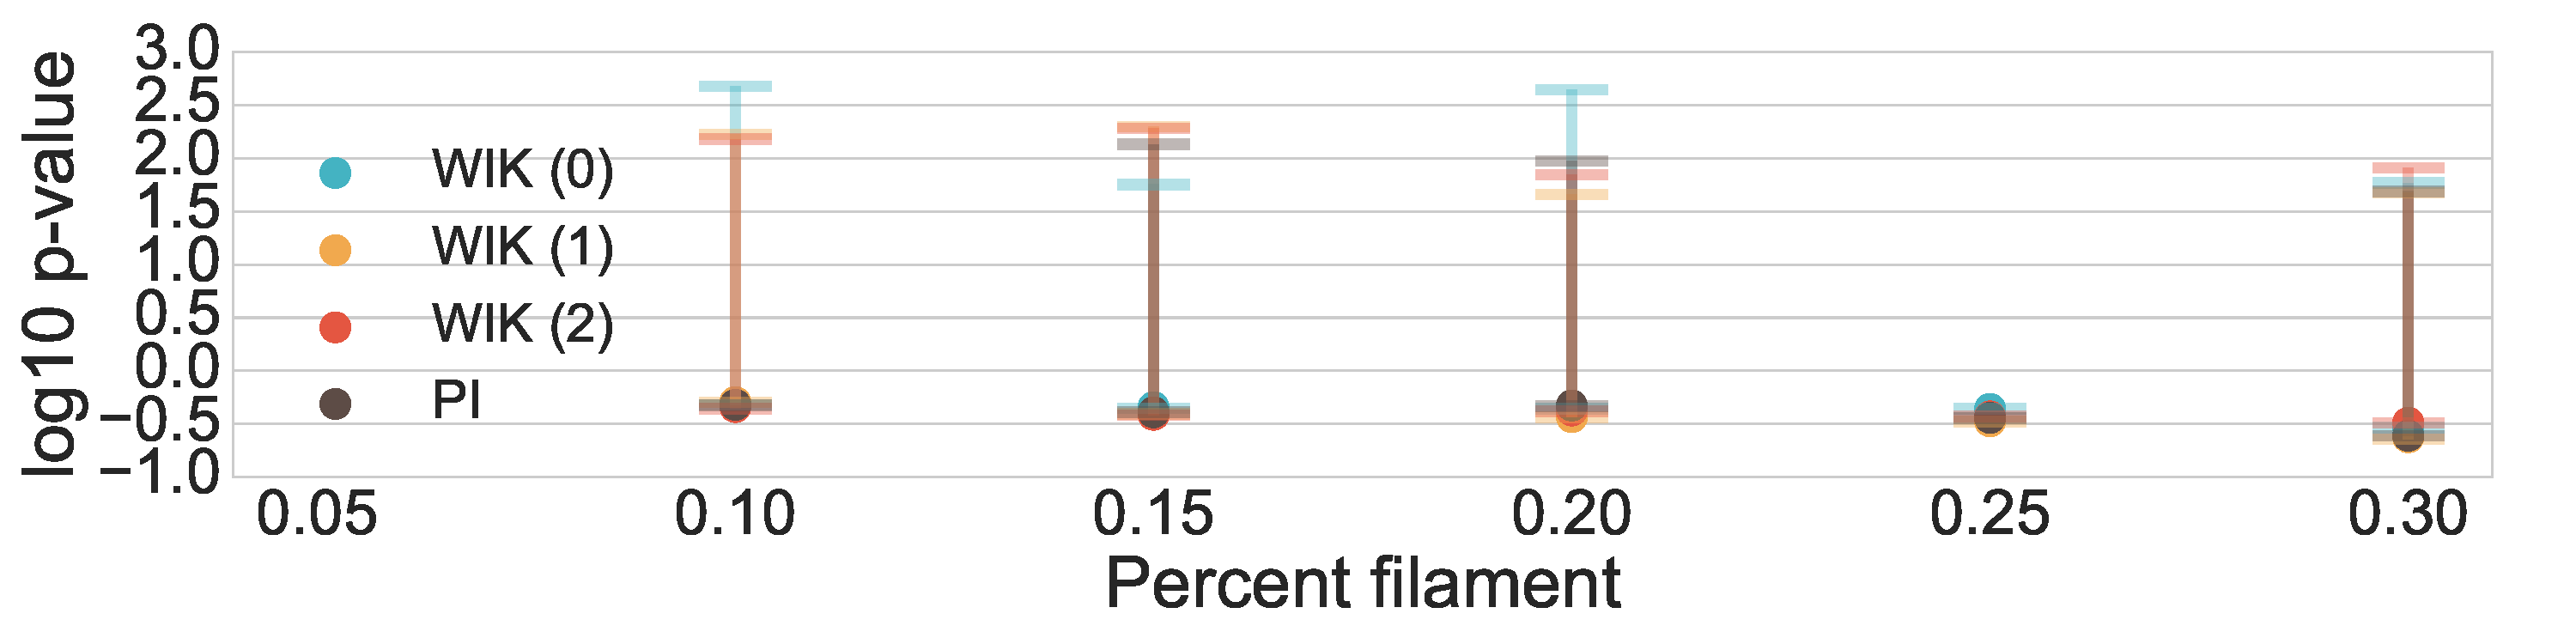
\includegraphics[width=\linewidth]{figure_8_weighted_contour_group_normed.pdf}
    \label{fig:sub_weight_normed}
  \end{subfigure}
\label{fig:sub_weight_results}
\caption{P-values from a suite of WIK tests.}
\end{figure}

\begin{figure}[htp!]
  \centering
  \begin{subfigure}{.8\textwidth}
    \caption{CORR Tests}
    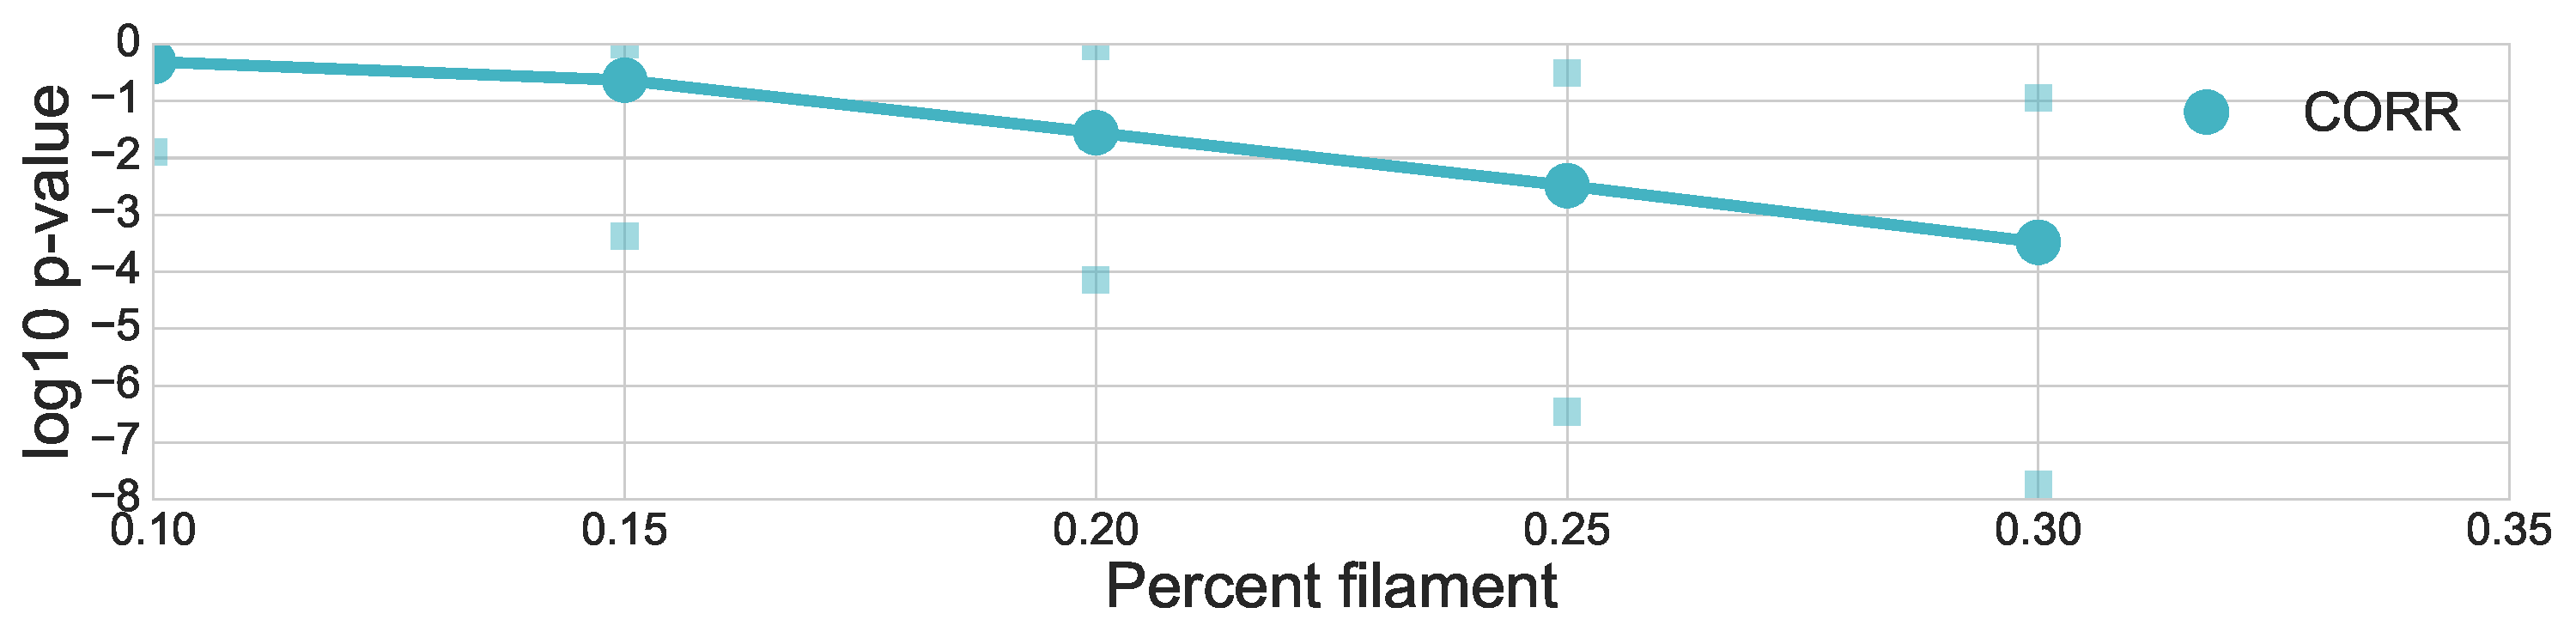
\includegraphics[width=\linewidth]{figure_8_correlation_group.pdf}
    \label{fig:sub_corr}
  \end{subfigure}
  \begin{subfigure}{.8\textwidth}
    \caption{CORR Tests (Normed)}
    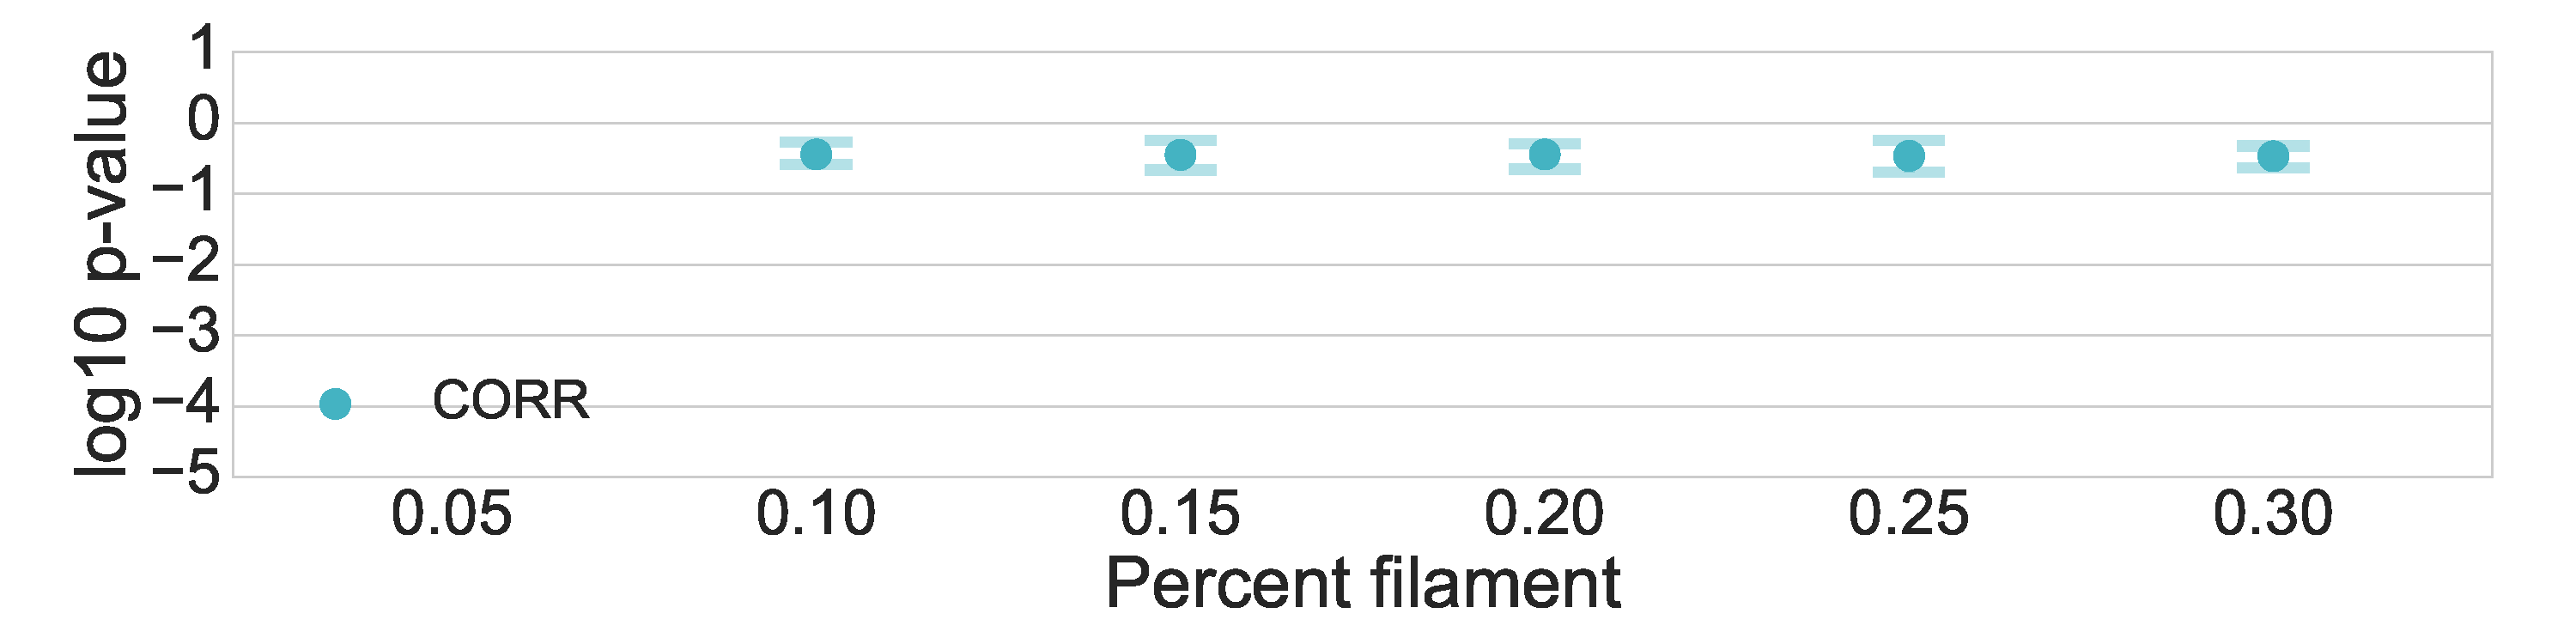
\includegraphics[width=\linewidth]{figure_8_correlation_group_normed.pdf}
    \label{fig:sub_corr_normed}
  \end{subfigure}
\caption{P-values from a suite of CORR tests.}
\label{fig:sub_corr_results_2}
\end{figure}

From \figref{fig:sub_euler_results} to \figref{fig:sub_corr_results_2}, we see that the EC test, the CORR test, and the SilEC test are the most effective (in that order) in distinguishing differences between the Voronoi simulations. All other tests are not as sensitive, eventually finding differences between the test and control once percfil is around 0.7 (see Appendix). Additionally, all tests derived from Euler characteristics perform relatively well compared to the other tests, suggesting that the Betti numbers, by being topologically invariant, are much better functional summaries of the persistence diagrams than intensity functions, silhouettes, and landscapes. More interestingly, it is possible that the alternating linear function by which the Betti numbers are combined may better preserve topological information given that the SilEC test, which combines silhouettes through a similar linear fashion, performed better than any individual silhouette counterpart and the naive cross-dimension combination (SIL (0:2)). Finally, the CORR test, being independent of persistence diagrams, acts as an powerful alternative to the EC test, being nearly as sensitive as percFil increases.

\subsubsection{Standardization of persistence diagrams} \label{sec:standardize}
In the methods proposed above, difference in scale can also result in rejection when, in fact there are not statistically significant topological differences. For example, suppose we are considering two datasets - each has points randomly sampled from the perimeter of a circle with a radius of 1 and 10 respectively. It may or may not be desirable to conclude that the two datasets come from different persistence diagram generators (i.e. conclude $\mathcal P^{(1)} \neq \mathcal P^{(2)}$) since inference would be based on geometrical (scaling) differences rather than topological differences. If we wish to focus only on topological differences, we propose a possible preprocessing step to normalize scaling. Specifically, we standardize the persistence diagrams so that all the homological features are re-scaled to $[0, 1]\times[0,1]$. This simple standardization takes the persistence diagram window and shrinks it or expands it to fill the $[0, 1]\times[0,1]$ window, maintaining the same relationship among all the homological features. If there is concern about outliers, then other quantiles could be used for the standardization. The exception is with the CORR, in which the point cloud itself is standardized to $[0, 1]\times[0, 1]\times[0, 1]$.

We repeated the simulation study from Section~\ref{sec:results1} except including our standardization; the results are displayed in \figref{fig:linesUnnormApp}. Standardization had an appreciable impact on hypothesis test results, decreasing the effectiveness and sensitivity of all test statistics. Notice, however, that the best-performing test statistics remain the same: EC, CORR, SILEC tests, confirming that the properties underlying those three tests are better able to capture purely topological differences than any other test presented in this paper. Notably after standardization, the KC, WIK, and other Sil tests have essentially constant p-values across the percFil variation, losing almost all effectiveness in distinguishing differences. One interpretation may be that these tests captured only geometric dissimilarities in the unstandardized setting.

%%%%%%%%%%%%%%%%%%%%%%%%%%%%%%%%%%%%%%%%%%%%%%%%%%%%%%%
%% SECTION: APPLICATION
%%%%%%%%%%%%%%%%%%%%%%%%%%%%%%%%%%%%%%%%%%%%%%%%%%%%%%%

\section{Application: Cosmological Simulation Data}
\label{sec:application}

Similar to the simulation models from Section~\ref{sec:sim_model}, Megaparsec cosmic mass distributions are likewise characterized by intricate multiscale configuration of web-like filaments and voids. We apply the proposed methodology to cosmological simulation data.

{\color{red}
\begin{itemize}
\item  Discuss LSS
\item  Discuss Cosmological simulations
\item  Discuss Warm vs. Cold DM
\end{itemize}
Real observations of cosmic web:  Great Wall \citep{geller1989mapping}, Sloan Great Wall \citep{gott2005map}, gas \citep{cantalupo2014cosmic}.}

\begin{figure}[htp!]
  \centering
  \begin{subfigure}{0.25\textwidth}
    \centering
        \caption{Slice 1/64}
  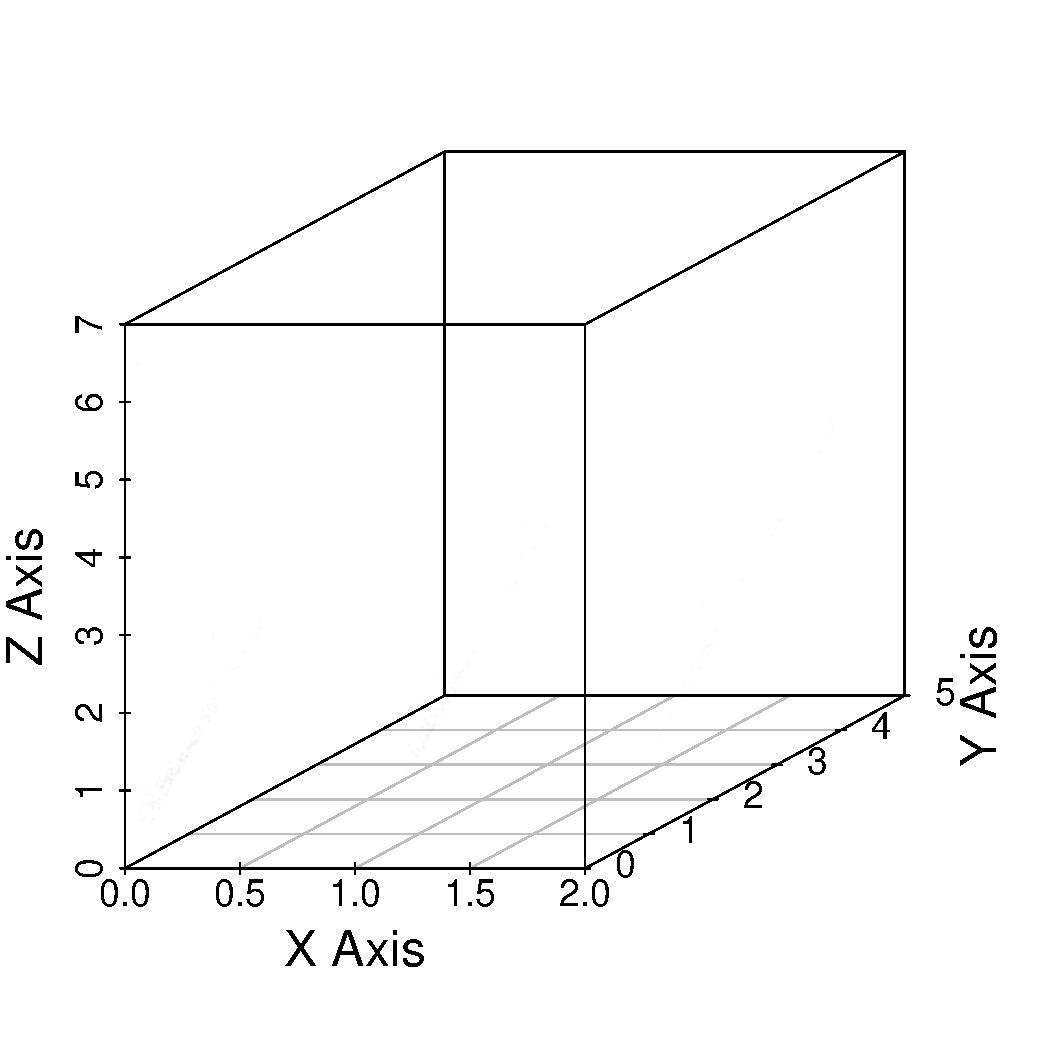
\includegraphics[width=\linewidth]{figure_10_cdm_slice_17.pdf}
    \label{fig:cubeDiagsA}
  \end{subfigure}
    \begin{subfigure}{0.25\textwidth}
    \centering
        \caption{Slice 8/64}
  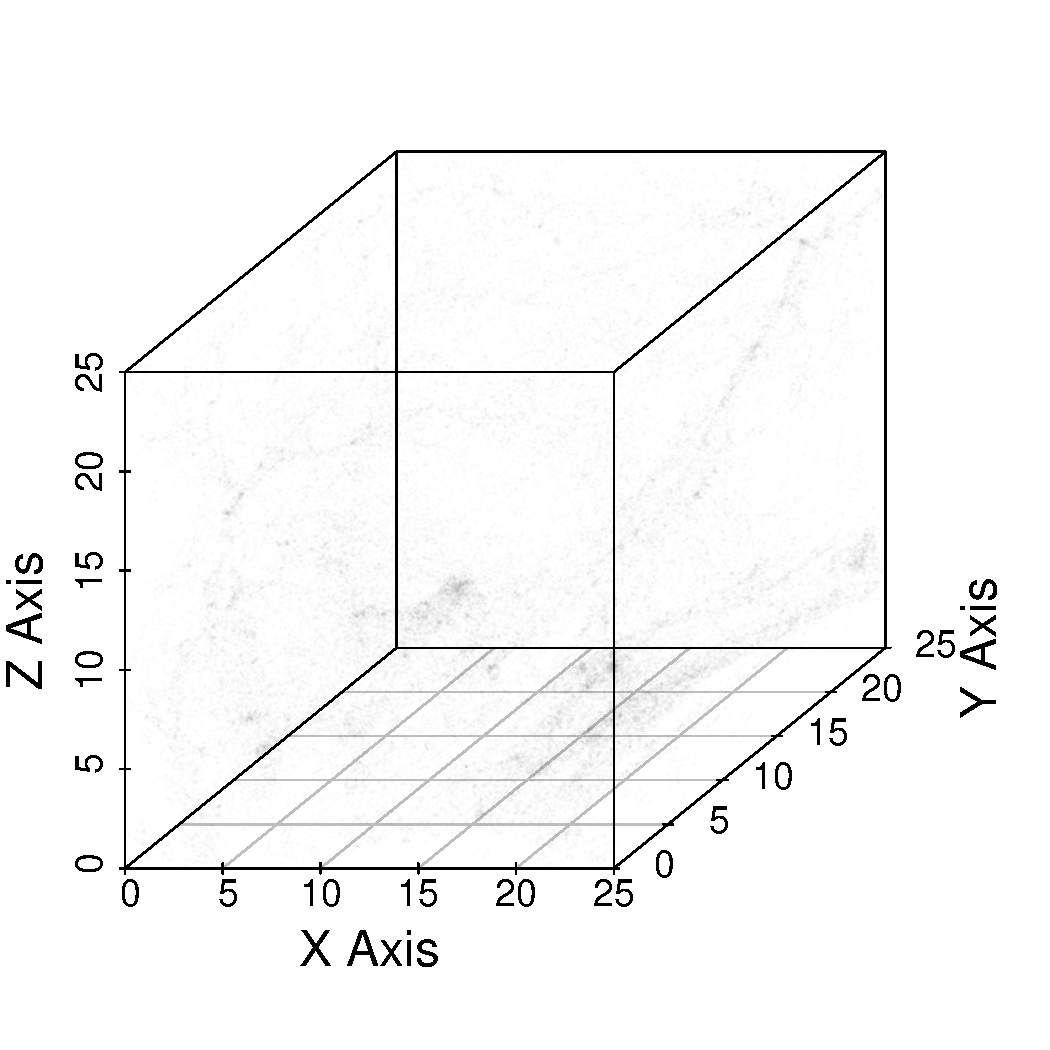
\includegraphics[width=\linewidth]{figure_10_cdm_slice_34.pdf}
    \label{fig:cubeDiagsB}
  \end{subfigure}
    \begin{subfigure}{0.25\textwidth}
    \centering
        \caption{Slice 55/64}
  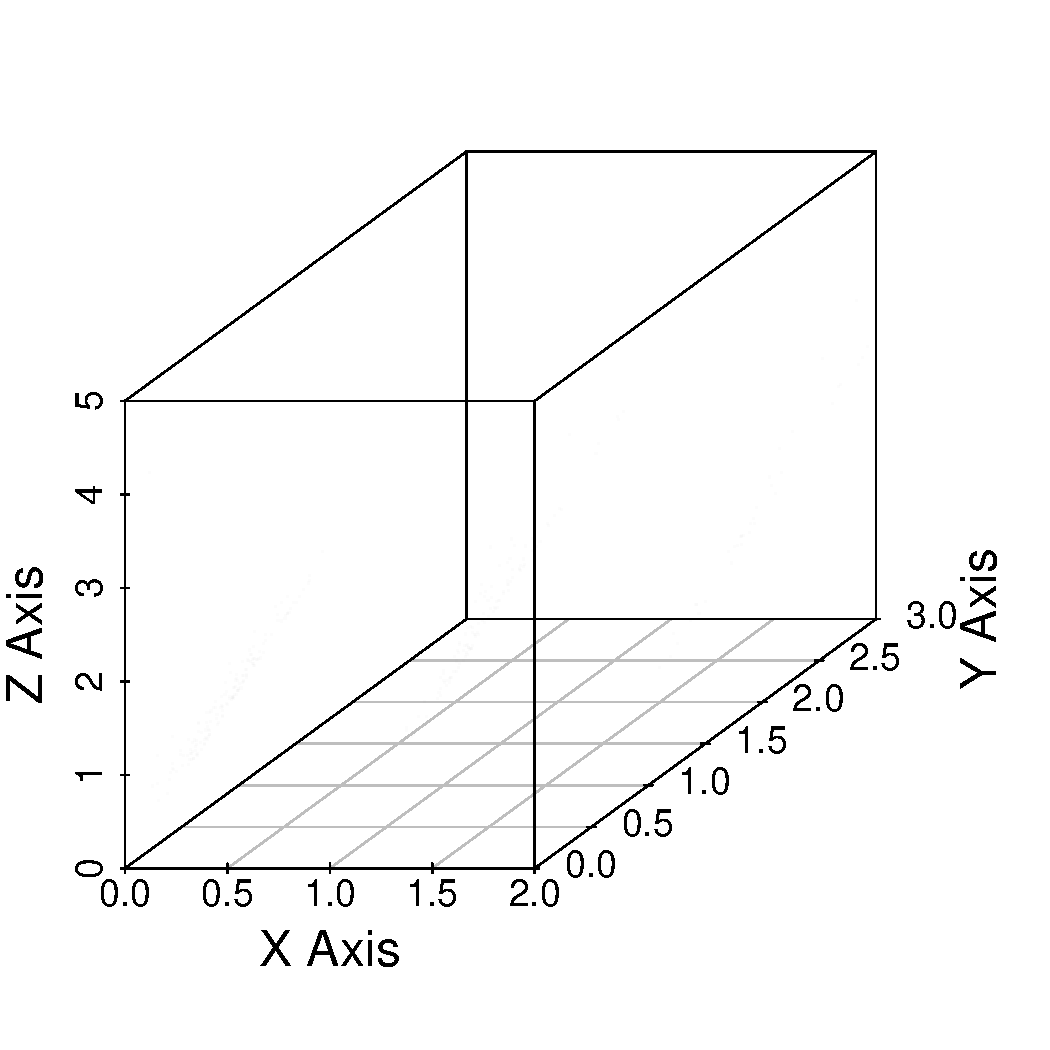
\includegraphics[width=\linewidth]{figure_10_cdm_slice_51.pdf}
    \label{fig:cubeDiagsC}
  \end{subfigure}
    \caption{Examples of three quadruple-split samples from a CDM simulation. Each of the three figures represents $\frac{1}{64}$th of a piece of the entire EAGLE CDM simulation.}
    \label{fig:cubeDiags}
\end{figure}

One parameter of interest is the state of the dark matter in the LSS. WDM and CDM are traditionally believed to produce very different realizations of the observable Universe, with the latter involving more slowly moving particles prone to produce a more lumpy distribution of galaxies and clusters. The former, containing more kinetic energy, has higher resistance to formation of global structure, and is theorized to render a less topologically-interesting cosmic mass. Applying the hypothesis testing framework would offer a method to \emph{quantify} the topological differences between simulations with underlying WDM and CDM assumptions.

For our two cosmological simulation cubes, one might consider cutting up the cubes into sub-cubes to bootstrap similar sets of samples as used in the Voronoi experiments. Let a \textit{double-split} be defined as splitting the simulation cube along both the $x$ and $y$ axis, creating 4 equally sized cubes in total. Similarly, a \textit{quadruple-split} produces 64 equally sized cubes, further splitting each of the cubes in a \textit{double-split} set into four sub-cubes. Using this splitting technique on both the CDM and WDM simulations, we end up with two usable data sets similar to the Voronoi Foam. However, by artifically expanding our data set, the WDM and CDM data sets are correlated due to their identical initial conditions. Because of this, the skeleton structure of the warm and cold DM simulations are nearly identical, allowing for paired T-tests. Note that there is also correlation between the samples due to the large-scale structure crossing the boundaries of the sub-cubes. We investigate this by changing the sizes of the sub-cubes, but consequently by doing so, decreases our sample size.

\subsection{The EAGLE project}
We analyze N-body simulations of structure formation. The simulation box is 100 co-moving Mpc on a side, and the numerical integration of the gravitational forces is run from redshift 127, when the age of the Universe is assumed to be less than 10Myr, to the present day (13.8 Gyr). The cosmological parameters are consistent with the 7-year results from the WMAP satellites: matter density $\Omega_0 = 0.272$, dark energy density $\Omega_{\Lambda} = 0.728$, Hubble parameter $h_0 = 0.704$, spectral index $n_s=0.967$, and power spectrum normalization $\sigma_8=0.81$. The mass of the simulation particle is $8.8x10^6$ $M_{sun}$. Haloes and subhaloes were identified using the SUBFIND algorithm \citep{springel2001populating}, and the smallest halo that can be resolved has 20 particles. These runs were performed to be dark matter-only counterparts to the the hydrodynamical runs of the Eagle project \citep{schaye2015eagle}; we stress that the runs used in this paper use gravity alone.

\begin{figure}[htp!]
  \centering
  \begin{subfigure}{0.24\textwidth}
    \caption{Eagle CDM}
    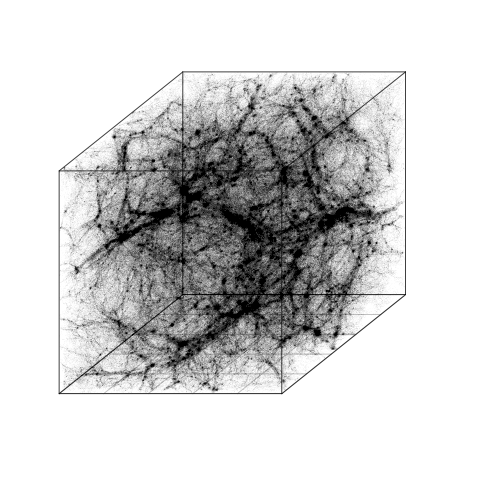
\includegraphics[width=\linewidth]{figure_11_cdm_plot.png}
    \label{fig:eagleDiagsA}
  \end{subfigure}
  \begin{subfigure}{0.24\textwidth}
    \caption{Eagle WDM}
    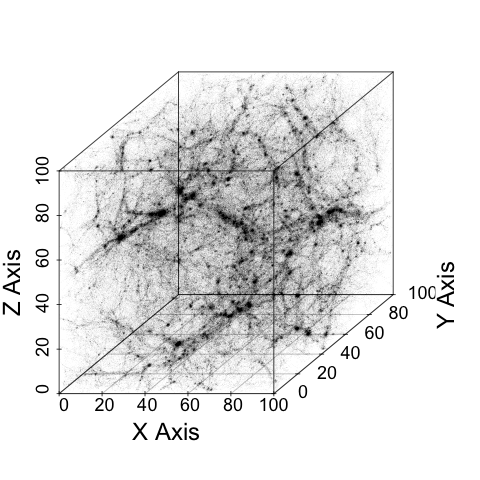
\includegraphics[width=\linewidth]{figure_11_wdm_plot.png}
    \label{fig:eagleDiagsB}
  \end{subfigure}
  \begin{subfigure}{0.24\textwidth}
    \caption{Eagle CDM PD}
    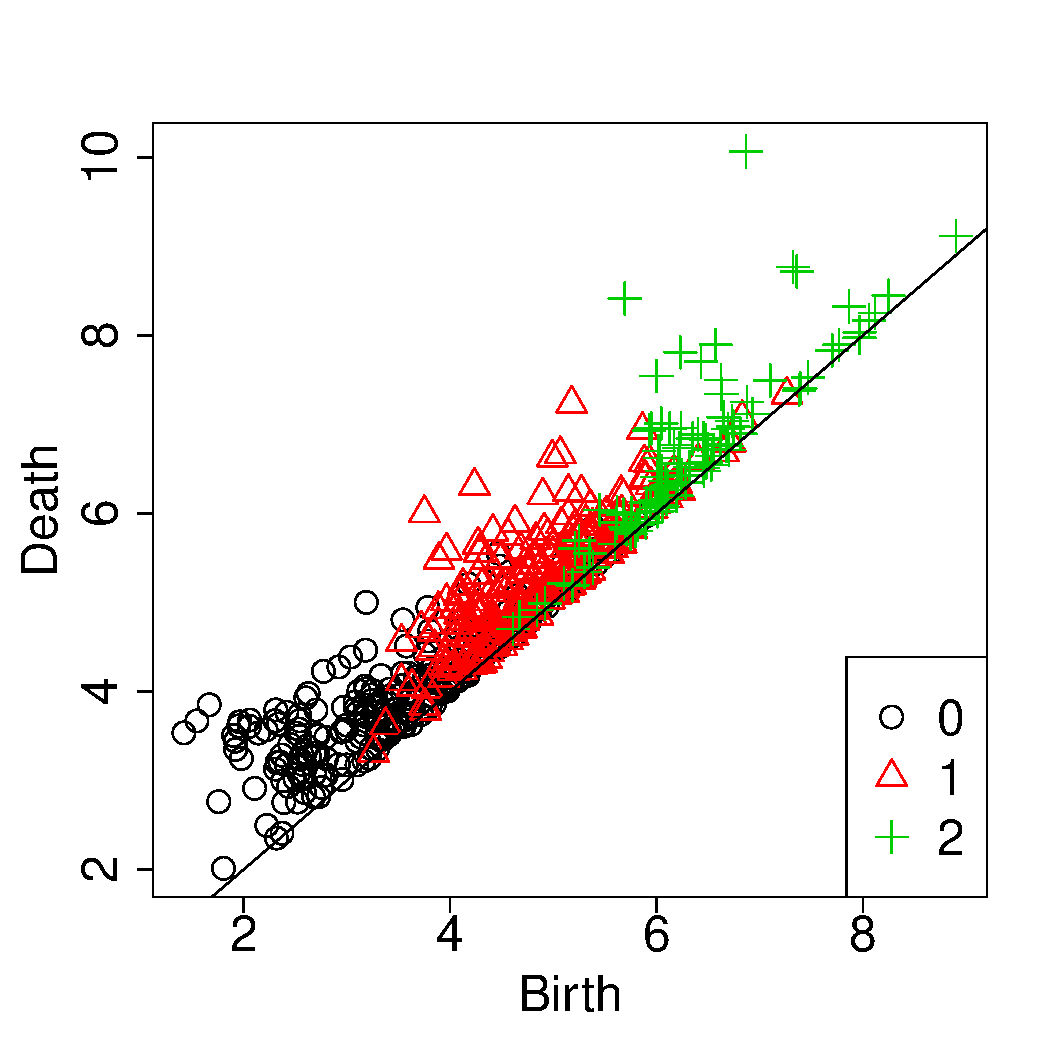
\includegraphics[width=\linewidth]{figure_11_cdm_pd.pdf}
    \label{fig:eagleDiagsC}
  \end{subfigure}
  \begin{subfigure}{0.24\textwidth}
    \caption{Eagle WDM PD}
    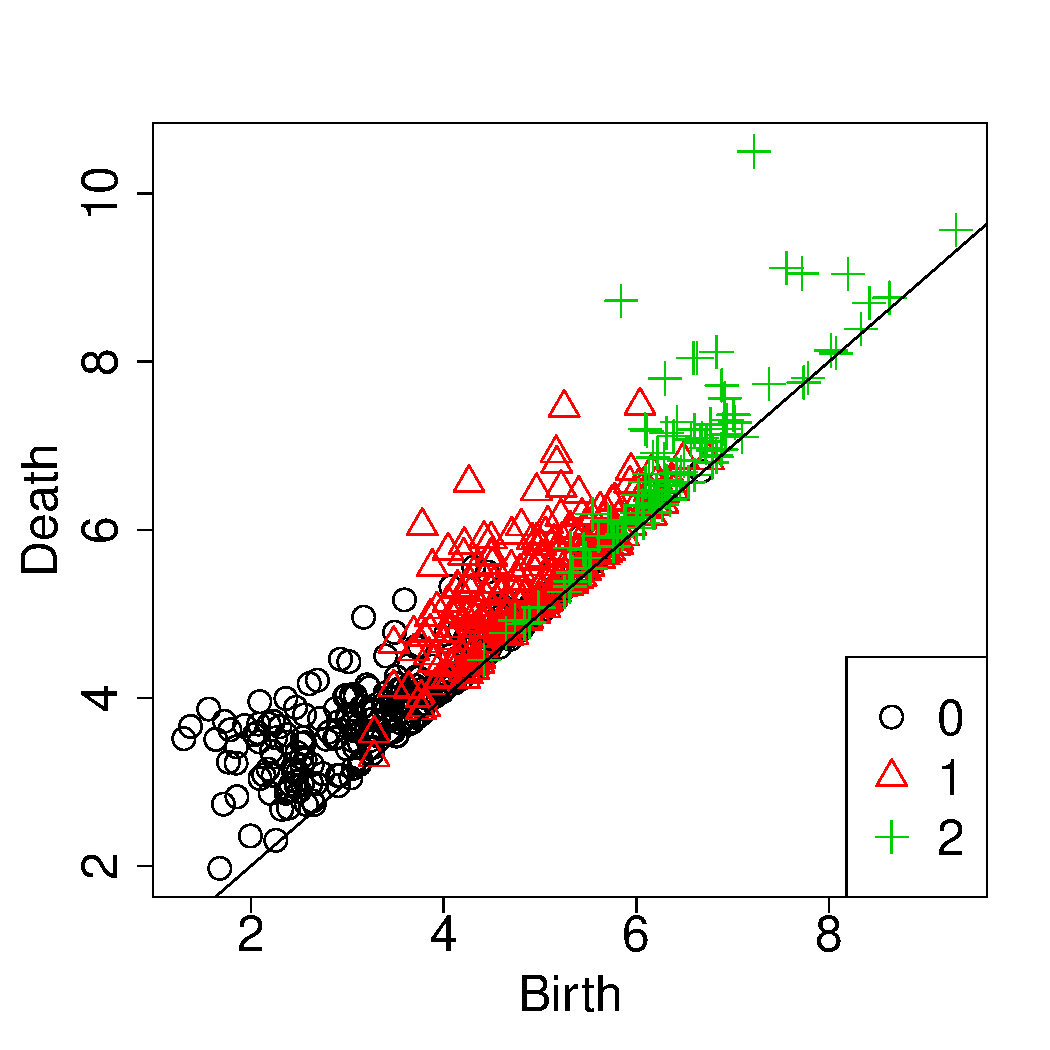
\includegraphics[width=\linewidth]{figure_11_wdm_pd.pdf}
    \label{fig:eagleDiagsD}
  \end{subfigure}
  \caption{(a, b) Point clouds of the complete EAGLE CDM and WDM simulations. (c, d) Their corresponding persistence diagrams. Although the CDM structure is denser, the persistence diagrams appear comparable. See the results of the hypothesis testing for more details.}

  \label{fig:eagleDiags}
\end{figure}

Both the CDM and WDM simulations make use of the same initial phases, and differ in that the latter has wave amplitudes rescaled using the transfer function of a 3.3keV thermal relic, with the relic mass chosen to be in agreement with the Lyman-alpha constraints of \citep{viel2013warm}. This results in the suppression of structure on the scale of dwarf galaxies. Spurious subhaloes have been removed using the algorithm of \citep{lovell2014properties}. \figref{fig:eagleDiags} shows a scatter plot of both the CDM and WDM simulations along with their respective persistent diagrams. Visually, we can confirm that the CDM is far more dense than WDM but seem to share similar internal structure; the persistence diagrams also share a general structure but we can identify smaller differences in homology groups that we hope to quantify using the hypothesis testing framework. These diagrams were generated under a volume of $1\times 10^{6}$, resolution of $2$ and a DTM distance function with hyper-parameter $0.001$.

\subsection{Results}
Table \ref{table:hypoCDMWDMresults} shows both the standardized (right) and unstandardized (left) results of the five categories of hypothesis tests. The unstandardized results suggest that with a higher number of splits, we are able to focus on smaller-scale topology, finding more significant differences. Through standardizing the persistence diagrams, we see that all the frameworks produce higher p-values on average and are less confident in the difference between double-split and quadruple-split datasets. This seems to explain that similar to the Voronoi foams, a large degree of the difference between WDM and CDM assumptions in the LSS are due to geometrical properties such as size. Judging from our most sensitive test statistics, Table \ref{table:hypoCDMWDMresults} suggest that statistically significant differences in topology exist between WDM and CDM realizations.

\begin{table}[htp!]
    \begin{center}
        \begin{tabular}{ l | c | c }
          \toprule
          \multicolumn{3}{c}{Unstandardized} \\
          \toprule
          Test & Double Split & Quadruple Split \\
          \midrule
          EC & 1.156e-06 & 7.379e-26 \\
          $\textup{EC}_{0:2}$ & 2.104e-05 & 7.379e-28 \\
          $\textup{EC}_{0}$ & 3.273e-08 & 3.811e-30 \\
          $\textup{EC}_{1}$ &  1.849e-05 & 0.935 \\
          $\textup{EC}_{2}$ & 0.340 & 0.0877 \\
          \midrule
          $\textup{Sil}_{\textup{EC}}$ & 7.709e-08 & 2.455e-20 \\
          $\textup{Sil}_{0:2}$ & 1.892e-06 & 1.114e-33 \\
          $\textup{Sil}_{0}$ & 2.958e-08 & 1.489e-34 \\
          $\textup{Sil}_{1}$ & 1.169e-05 & 2.884e-23 \\
          $\textup{Sil}_{2}$ & 0.925 & 0.0345 \\
          \midrule
          $\textup{KC}_{0}$ & 0.442 & 0.000 \\
          $\textup{KC}_{1}$ & 0.192 & 0.000 \\
          $\textup{KC}_{2}$ & 0.248 & 0.00199 \\
          \midrule
          $\textup{WIK}_{0}$ & 0.084 & 0.000 \\
          $\textup{WIK}_{1}$ & 0.051 & 0.000 \\
          $\textup{WIK}_{2}$ & 0.496 & 0.000 \\
          $\textup{PI}$ & 0.923 & 0.281 \\
          \midrule
          $\textup{CORR}$ & 6.656e-04 & 7.355e-16 \\
          \bottomrule
        \end{tabular}
        \begin{tabular}{ l | c |  c }
          \toprule
          \multicolumn{3}{c}{Standardized} \\
          \toprule
          Test & Double Split & Quadruple Split \\
          \midrule
          EC & 1.102e-04 &  7.345e-12 \\
          $\textup{EC}_{0:2}$ & 1.327e-05 &  3.972e-14 \\
          $\textup{EC}_{0}$ & 1.387e-06 & 1.614e-12 \\
          $\textup{EC}_{1}$ & 0.0235 & 0.00143 \\
          $\textup{EC}_{2}$ & 0.00385 & 1.977e-07 \\
          \midrule
          $\textup{Sil}_{\textup{EC}}$ & 0.0122 & 0.00500 \\
          $\textup{Sil}_{0:2}$ & 4.295e-04 & 8.072e-12 \\
          $\textup{Sil}_{0}$ & 6.471e-06 & 1.762e-11 \\
          $\textup{Sil}_{1}$ & 0.0282 & 3.899e-07 \\
          $\textup{Sil}_{2}$ & 0.00294 & 1.545e-04 \\
          \midrule
          $\textup{GC}_{0}$ & 0.986 & 0.856 \\
          $\textup{GC}_{1}$ & 0.962 & 0.956 \\
          $\textup{GC}_{2}$ & 0.962 & 0.260 \\
          \midrule
          $\textup{WIK}_{0}$ & 0.092 & 0.000 \\
          $\textup{WIK}_{1}$ & 0.066 & 0.000 \\
          $\textup{WIK}_{2}$ & 0.459 & 0.001 \\
          $\textup{PI}$ & 0.999 & 0.306 \\
          \midrule
          $\textup{CORR}$ & 0.0289 & 0.918 \\
          \bottomrule
        \end{tabular}
    \end{center}
\caption{P-values from hypothesis tests on the unstandardized (left) and standardized (right) WDM \& CDM simulations by double, and quadruple splits. A p-value of $0.000$ comes from a permutation test with no positive examples. As the number of splits increases, the p-values dramatically decrease for the unstandardized setting, suggesting small-scale geometric and topological differences. A similar pattern is present, though less pronounced in the standardized setting.}
\label{table:hypoCDMWDMresults}
\end{table}

\subsection{Localizing Differences}
A question after discovering that differences exist in both geometry and topology is how are these differences distributed? One hypothesis might be that the differences are grouped among clustered sections of the observable Universe while other galaxies are practically identical. It is also possible that the differences are uniformly distributed across our cosmic data. To explore these questions more, we looked at the Bottleneck distances between different cubic splits as the number of splits increased. Because a higher number of splits focuses on smaller parts of the CDM/WDM simulation, we expect higher resolution into the topological features specific to that region. \figref{fig:cubeHeatmap} shows 3 sets of heatmaps for each of the 3 persistent homologies. Each set includes another 3 heatmaps, detailing the Bottleneck distances between congruent CDM and WDM unsplit, double-split, and quadruple-split partitions respectively.

\begin{figure}[htp!]
  \centering
  \begin{subfigure}{.45\textwidth}
    \centering
    \caption{Dimension 0 Heatmap Set}
    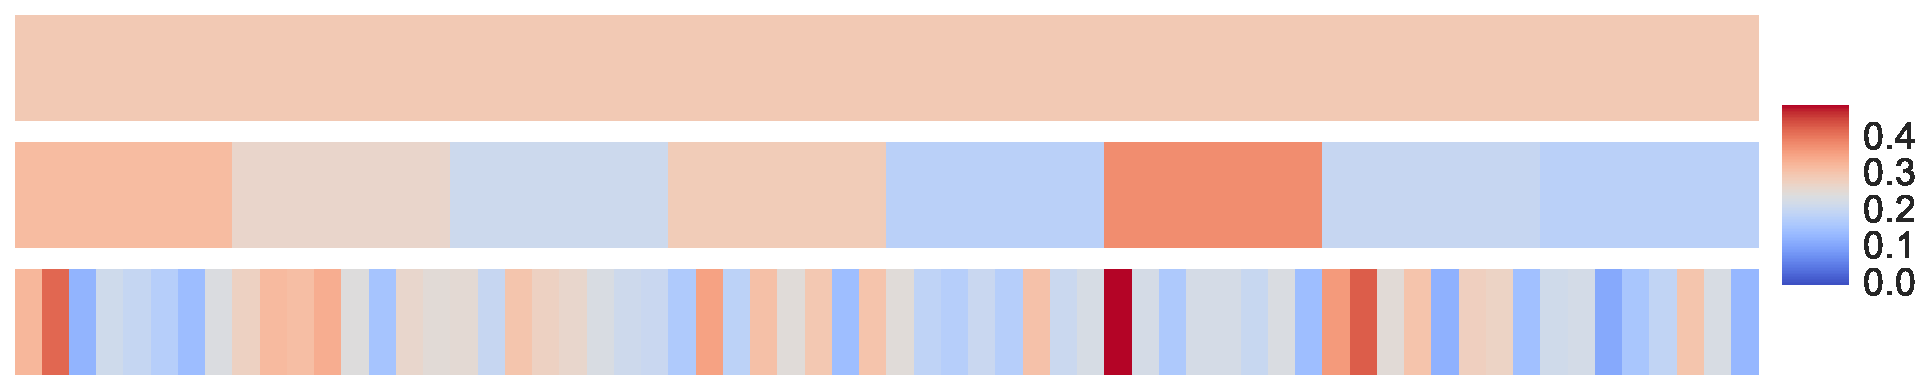
\includegraphics[width=\linewidth]{fig_12_hmap_dim0_nonorm.pdf}
    \label{fig:cubeHeatmap0}
  \end{subfigure}
  \begin{subfigure}{.45\textwidth}
    \centering
    \caption{Dimension 0 Standardized Heatmap Set}
    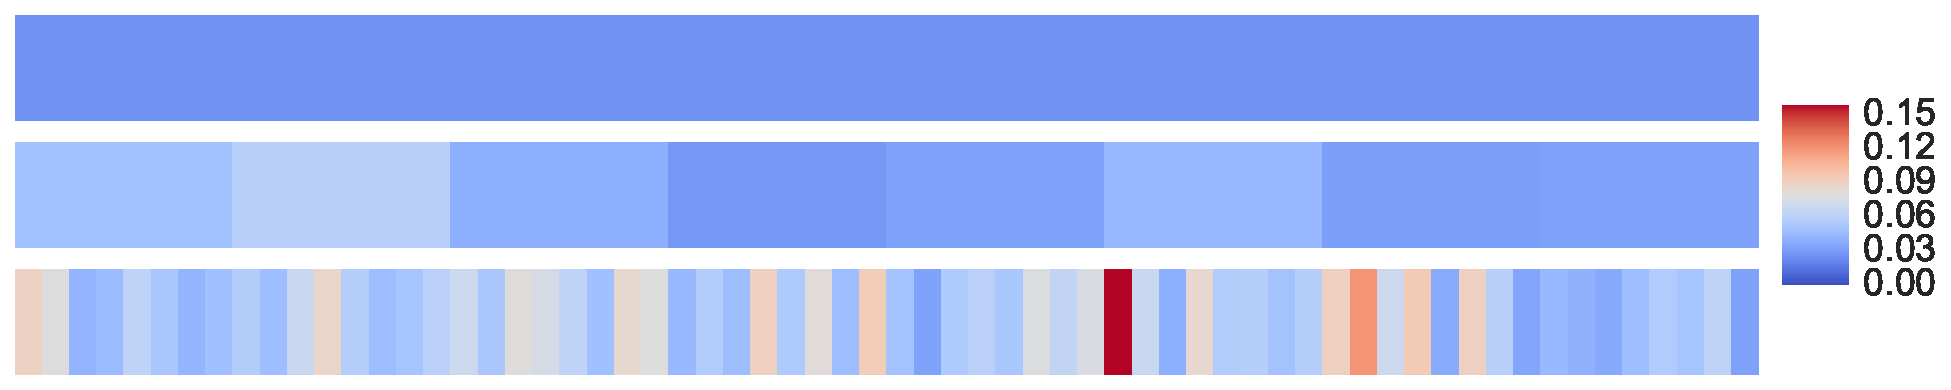
\includegraphics[width=\linewidth]{fig_12_hmap_dim0_yesnorm.pdf}
    \label{fig:cubeHeatmapStand0}
  \end{subfigure}
  \begin{subfigure}{.45\textwidth}
    \centering
    \caption{Dimension 1 Heatmap Set}
    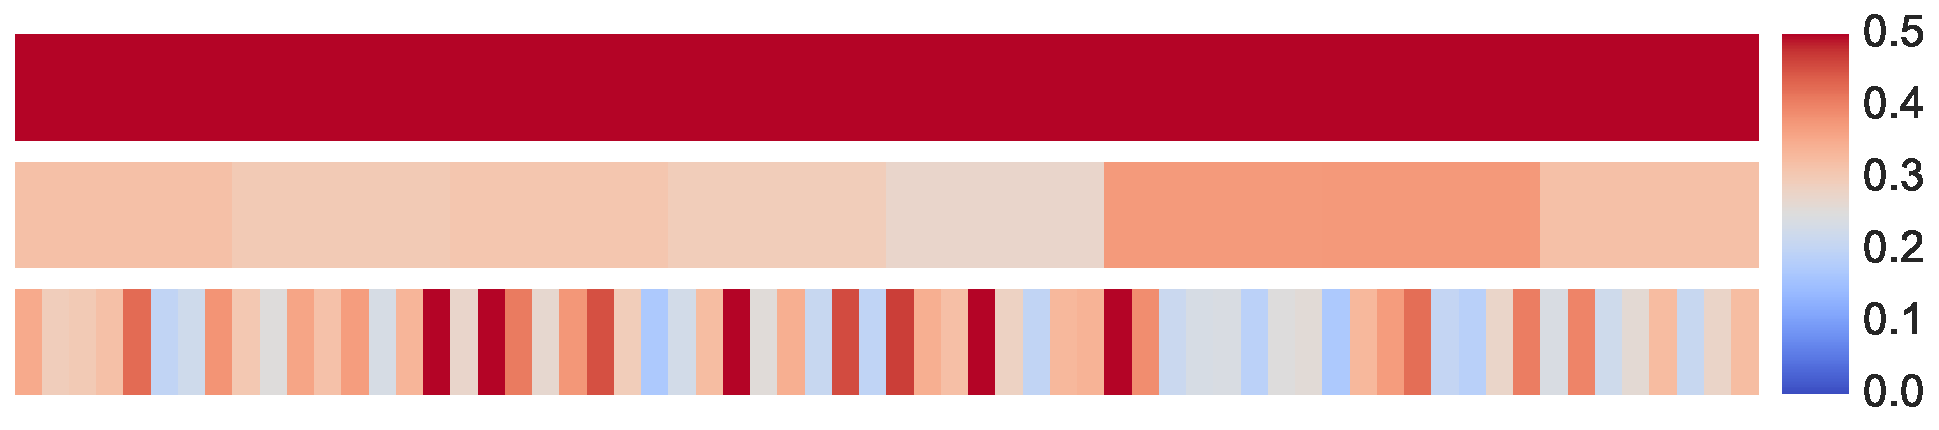
\includegraphics[width=\linewidth]{fig_12_hmap_dim1_nonorm.pdf}
    \label{fig:cubeHeatmap1}
  \end{subfigure}
  \begin{subfigure}{.45\textwidth}
    \centering
    \caption{Dimension 1 Standardized Heatmap Set}
    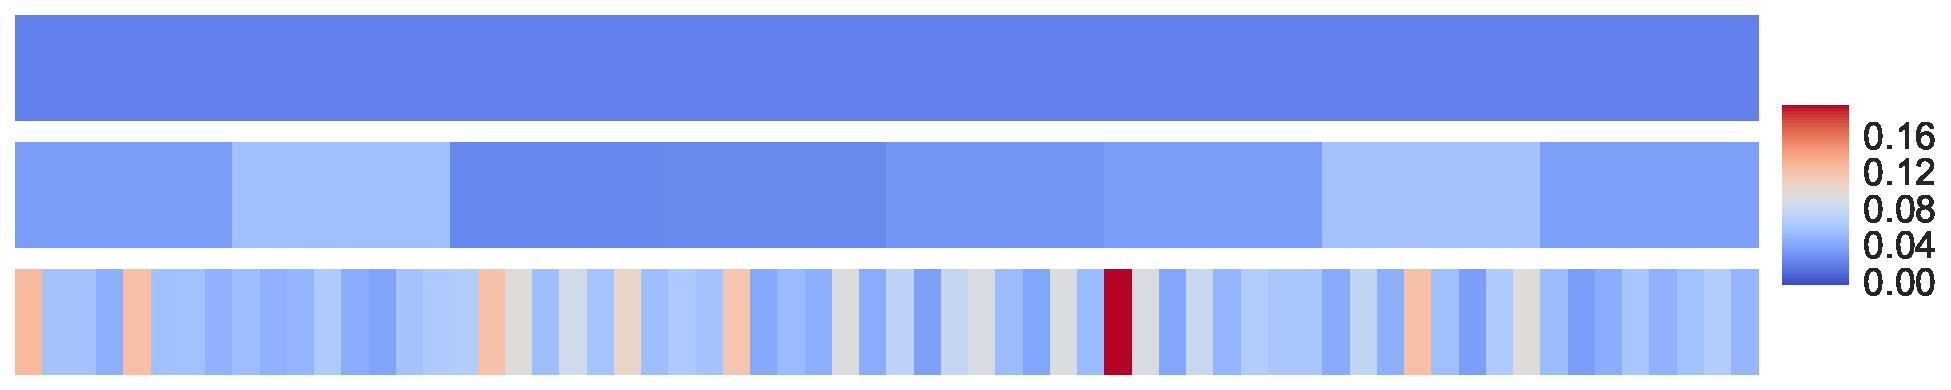
\includegraphics[width=\linewidth]{fig_12_hmap_dim1_yesnorm.pdf}
    \label{fig:cubeHeatmapStand1}
  \end{subfigure}
  \begin{subfigure}{.45\textwidth}
    \centering
    \caption{Dimension 2 Heatmap Set}
    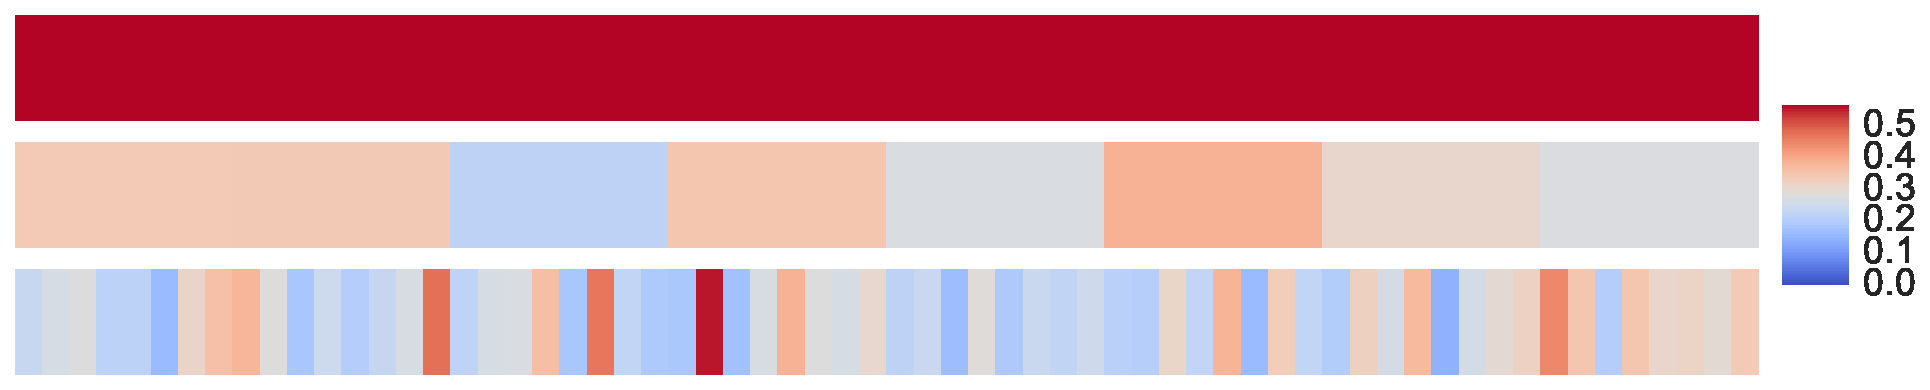
\includegraphics[width=\linewidth]{fig_12_hmap_dim2_nonorm.pdf}
    \label{fig:cubeHeatmap2}
  \end{subfigure}
  \begin{subfigure}{.45\textwidth}
    \centering
    \caption{Dimension 2 Standardized Heatmap Set}
    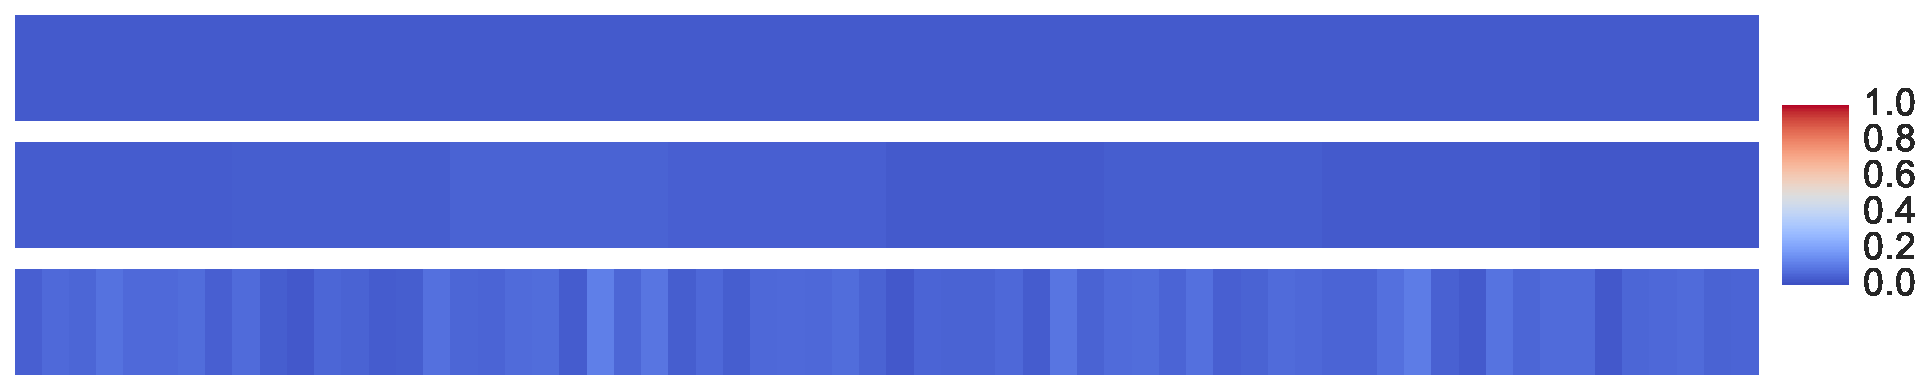
\includegraphics[width=\linewidth]{fig_12_hmap_dim2_yesnorm.pdf}
    \label{fig:cubeHeatmapStand2}
  \end{subfigure}
  \caption{Each subfigure (a-f) contains three horizontal heatmaps representing (from top to bottom) the Bottleneck distances between each slice of unsplit, double split, and quadruple split pairs from respective WDM and CDM data sets by dimension. Each individual heatmap is a vectorization of the cubic slices produced from the WDM and CDM Eagle simulations. For example, \figref{fig:cubeHeatmap0}\'s top row contains only 1 slice, since the whole EAGLE simulation itself is one part; the second row contains 8 slices, since the dataset was split along two axis; similarly, the third row contains 64 slices. Subfigures (a, c, e) show the bottleneck distances derived from unstandardized persistence diagrams while the subfigures (b, d, f) use standardized diagrams.}
  \label{fig:cubeHeatmap}
\end{figure}

From \figref{fig:cubeHeatmap}, we might infer that the topological and geometric differences are certainly not uniform. For each of the three homologies, introducing a greater number of splits uncovers greater magnitudes of Bottleneck distances between CDM and WDM cubes. This suggests that it is possible for topological differences to be masked by local similarities from a global perspective. At the very least, we can be confident that there exist partitions of topologically similar areas and partitions of topologically dissimilar areas within the EAGLE simulation. Further work should explore what areas in the Universe occupy these two partitions and if there exist physical evidence of differences.

\begin{figure}[htp!]
  \centering
    \begin{subfigure}{0.21\textwidth}
    \centering
        \caption{EC (High)}
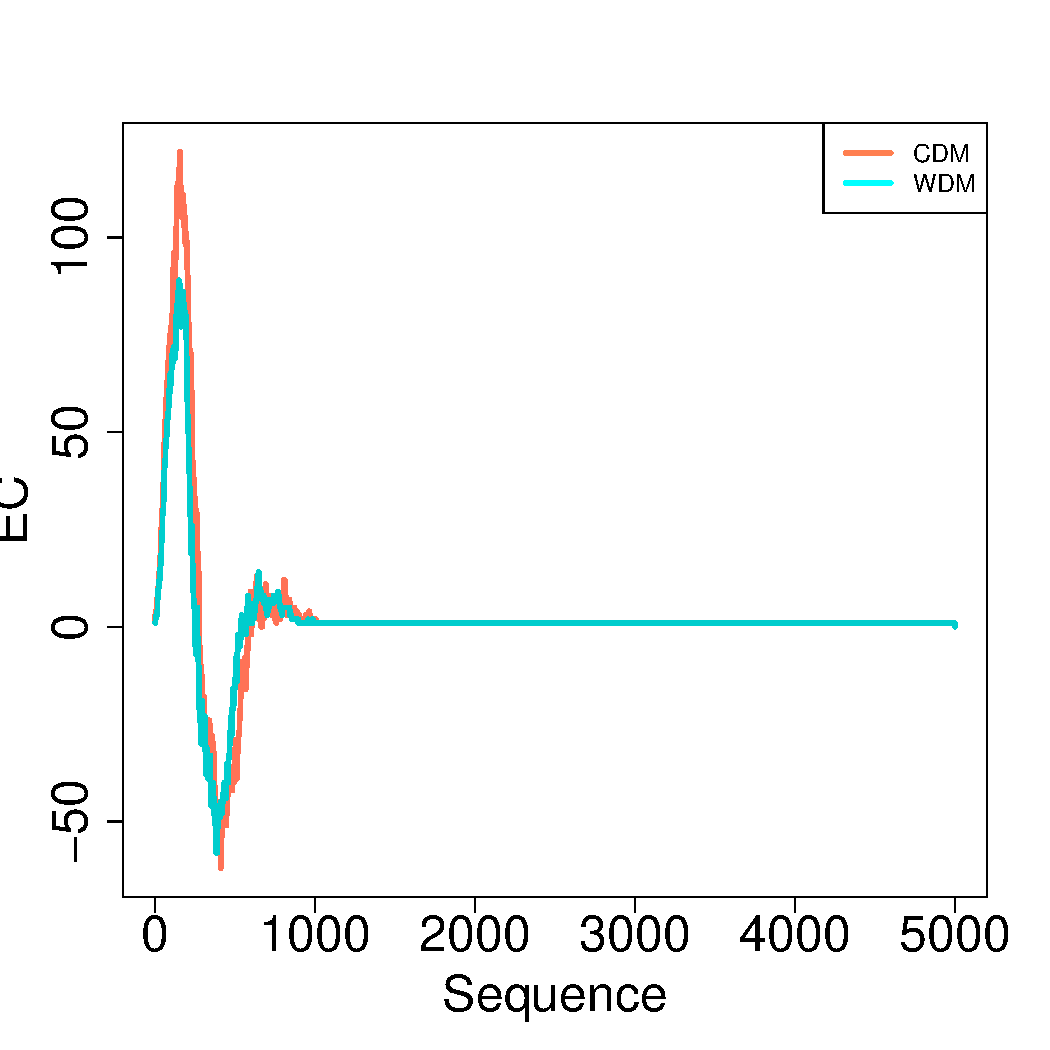
\includegraphics[width=\linewidth]{figure_13_max_margin_2euler.pdf}
    \label{fig:valid1}
  \end{subfigure}
    \begin{subfigure}{0.24\textwidth}
    \centering
        \caption{CORR (High)}
\includegraphics[width=\linewidth]{figure_13_max_margin_corr.pdf}
    \label{fig:valid2}
  \end{subfigure}
    \begin{subfigure}{0.21\textwidth}
    \centering
        \caption{EC (Low)}
\includegraphics[width=\linewidth]{figure_13_min_margin_2euler.pdf}
    \label{fig:valid3}
  \end{subfigure}
    \begin{subfigure}{0.24\textwidth}
    \centering
        \caption{CORR (Low)}
\includegraphics[width=\linewidth]{figure_13_min_margin_corr.pdf}
    \label{fig:valid4}
  \end{subfigure}
    \caption{A comparison of EC and CORR for dimension 1 between the cube with the highest bottleneck distance and the cube with the lowest. (a) and (b) clearly depict larger distinctions between the CDM (red) and WDM (blue) slices than (c) and (d).}
    \label{fig:validationfigs}
\end{figure}

Provided that EC and CORR were the two most effective hypothesis tests, to confirm the validity of these heatmaps, we compared these two functions for the unstandardized cubes with the highest Bottleneck distance and the unstandardized cubes with the lowest Bottleneck distance. As expected, \figref{fig:validationfigs} confirms that the (High) EC and (High) CORR functions have far more discrepancies than their (Low) counterparts, also suggesting that certain partitions are more similar topologically than others. The same pattern arises for dimension 0 and dimension 2.

We can do the same heatmap experiment with the standardized persistence diagrams. As confirmed in the hypothesis testing of both the Voronoi and the EAGLE simulations, standardizing removes geometric differences, greatly reducing the Bottleneck distances, as seen in \figref{fig:cubeHeatmap}(b,d,f). Notably, for dimensions 0 and 1, the cube with the largest bottleneck distance remained the same as in the unstandardized heatmaps, suggesting that those differences are largely not due to size, but true topological distinctions. Dimension 2, however, was less consistent, possibly indicating that voids in CDM and WDM are more aberrant in terms of size, not topological shape. Despite the differences standardizing induced, we are still confident that differences in topology alone are not uniform across the EAGLE Universe: certain splits are consistently indicating differences in dark matter make-up between warm and cold assumptions.

%%%%%%%%%%%%%%%%%%%%%%%%%%%%%%%%%%%%%%%%%%%%%%%%%%%%%%%
%% SECTION: CONCLUSION
%%%%%%%%%%%%%%%%%%%%%%%%%%%%%%%%%%%%%%%%%%%%%%%%%%%%%%%

\section{Conclusion}
\label{sec:conc}
In this paper, we presented a hypothesis testing framework built on persistent homology to compare topological summaries of two sets of point cloud data. We showed empirically that such a framework is able to infer differences in the true distribution of topology by comparing Voronoi tessellations with controlled hyperparameters. Additionally, we presented the application of this framework on the EAGLE data set to analyze the topology of the cosmic mass given assumptions of warm and cold dark matter, resulting in the discovering of locally significant spatial differences in geometry and topology. We believe this framework may provide a standard method for evaluating topological hypotheses in a diverse array of fields that greatly improve over currently existing methods.

%%%%%%%%%%%%%%%%%%%%%%%%%%%%%%%%%%%%%%%%%%%%%%%%%%%%%%%
%% SECTION: SUPPLEMENTS
%%%%%%%%%%%%%%%%%%%%%%%%%%%%%%%%%%%%%%%%%%%%%%%%%%%%%%%

\bigskip
\begin{center}
{\large\bf SUPPLEMENTARY MATERIAL}
\end{center}

\begin{description}
  \item[Additional voronoi simulations:] Hypothesis testing p-values for voronoi simulations of percent filament varying from 0.1 to 0.9. See \figref{fig:linesUnnormApp}.

  \begin{center}
    \begin{figure}[htp!]
      \centering
      \begin{subfigure}{.45\textwidth}
        \centering
        \caption{EC Tests}
        \includegraphics[width=\linewidth]{figure_8_all_euler_group.pdf}
        \label{fig:all_euler}
      \end{subfigure}
      \begin{subfigure}{.45\textwidth}
        \centering
        \caption{EC Tests (Normed)}
        \includegraphics[width=\linewidth]{figure_8_all_euler_group_normed.pdf}
        \label{fig:all_euler_normed}
      \end{subfigure}
      \begin{subfigure}{.45\textwidth}
        \centering
        \caption{SIL Tests}
        \includegraphics[width=\linewidth]{figure_8_all_silhouette_group.pdf}
        \label{fig:all_silh}
      \end{subfigure}
      \begin{subfigure}{.45\textwidth}
        \centering
        \caption{SIL Tests (Normed)}
        \includegraphics[width=\linewidth]{figure_8_all_silhouette_group_normed.pdf}
        \label{fig:all_silh_normed_normed}
      \end{subfigure}
      \begin{subfigure}{.45\textwidth}
        \centering
        \caption{IK Tests}
        \includegraphics[width=\linewidth]{figure_8_all_contour_group.pdf}
        \label{fig:all_contour}
      \end{subfigure}
      \begin{subfigure}{.45\textwidth}
        \centering
        \caption{IK Tests (Normed)}
        \includegraphics[width=\linewidth]{figure_8_all_contour_group_normed.pdf}
        \label{fig:all_contour_normed}
      \end{subfigure}
      \begin{subfigure}{.45\textwidth}
        \centering
        \caption{WIK/PI Tests}
        \includegraphics[width=\linewidth]{figure_8_all_weighted_contour_group.pdf}
        \label{fig:all_weight}
      \end{subfigure}
      \begin{subfigure}{.45\textwidth}
        \centering
        \caption{WIK/PI Tests (Normed)}
        \includegraphics[width=\linewidth]{figure_8_all_weighted_contour_group_normed.pdf}
        \label{fig:all_weight_normed}
      \end{subfigure}
      \begin{subfigure}{.45\textwidth}
        \caption{CORR Tests}
        \includegraphics[width=\linewidth]{figure_8_all_correlation_group.pdf}
        \label{fig:all_corr}
      \end{subfigure}
      \begin{subfigure}{.45\textwidth}
        \caption{CORR Tests (Normed)}
        \includegraphics[width=\linewidth]{figure_8_all_correlation_group_normed.pdf}
        \label{fig:all_corr_normed}
      \end{subfigure}
      \caption{P-values for EC, SIL, IK, WIK, PI, and CORR. X-axis represents a varying percent filament (0.1 to 0.9 with 0.1 step increments) being compared to a baseline of 0.1; Y-axis shows the p-values in $\textup{1og}_{10}$ space. The lines plot the median $\log_{10}$ p-value and peripheral points show the 25th and 75th percentile p-values of the 100 iterations. The right column of plots replicates the left with the exception of normalizing the persistence diagrams prior to testing. Points containing X marks indicate a p-value of 0.}
      \label{fig:linesUnnormApp}
    \end{figure}
  \end{center}
\end{description}

%%%%%%%%%%%%%%%%%%%%%%%%%%%%%%%%%%%%%%%%%%%%%%%%%%%%%%%
%% SECTION: REFERENCES
%%%%%%%%%%%%%%%%%%%%%%%%%%%%%%%%%%%%%%%%%%%%%%%%%%%%%%%

\bibliographystyle{agsm}
\bibliography{mybib}
\end{document}
